\documentclass{article}

%%% Begin Ryan's template
\usepackage[utf8]{inputenc} % allow utf-8 input
\usepackage[T1]{fontenc}    % use 8-bit T1 fonts
\usepackage{booktabs}       % professional-quality tables
\usepackage{nicefrac}       % compact symbols for 1/2, etc.
\usepackage{microtype}      % microtypography
\usepackage{times}          % times font

\usepackage[round]{natbib}
\usepackage{amssymb,amsmath,amsthm,bbm}
\usepackage[margin=1in]{geometry}
\usepackage{verbatim,float,url,dsfont}
\usepackage{graphicx,subfigure,psfrag}
\usepackage{algorithm,algorithmic}
\usepackage{mathtools,enumitem}
\usepackage[colorlinks=true,citecolor=blue,urlcolor=blue,linkcolor=blue]{hyperref}
\usepackage{multirow}

% Theorems and such
\newtheorem{theorem}{Theorem}
\newtheorem{lemma}{Lemma}
\newtheorem{corollary}{Corollary}
\newtheorem{proposition}{Proposition}
\theoremstyle{definition}
\newtheorem{remark}{Remark}
\newtheorem{definition}{Definition}

% Assumption
\newtheorem*{assumption*}{\assumptionnumber}
\providecommand{\assumptionnumber}{}
\makeatletter
\newenvironment{assumption}[2]{
	\renewcommand{\assumptionnumber}{Assumption #1#2}
	\begin{assumption*}
		\protected@edef\@currentlabel{#1#2}}
	{\end{assumption*}}
\makeatother

% Widebar
\makeatletter
\newcommand*\rel@kern[1]{\kern#1\dimexpr\macc@kerna}
\newcommand*\widebar[1]{%
	\begingroup
	\def\mathaccent##1##2{%
		\rel@kern{0.8}%
		\overline{\rel@kern{-0.8}\macc@nucleus\rel@kern{0.2}}%
		\rel@kern{-0.2}%
	}%
	\macc@depth\@ne
	\let\math@bgroup\@empty \let\math@egroup\macc@set@skewchar
	\mathsurround\z@ \frozen@everymath{\mathgroup\macc@group\relax}%
	\macc@set@skewchar\relax
	\let\mathaccentV\macc@nested@a
	\macc@nested@a\relax111{#1}%
	\endgroup
}
\makeatother

% Min and max
\newcommand{\argmin}{\mathop{\mathrm{argmin}}}
\newcommand{\argmax}{\mathop{\mathrm{argmax}}}
\newcommand{\minimize}{\mathop{\mathrm{minimize}}}
\newcommand{\st}{\mathop{\mathrm{subject\,\,to}}}

% Shortcuts
\def\R{\mathbb{R}}

%%% End Ryan's template

%%% Begin Alden's additions
\newcommand{\Ebb}{\mathbb{E}}
\newcommand{\Pbb}{\mathbb{P}}
\newcommand{\dotp}[2]{\langle #1, #2 \rangle}
\newcommand{\wt}[1]{\widetilde{#1}}
\newcommand{\wh}[1]{\widehat{#1}}
\newcommand{\mc}[1]{\mathcal{#1}}
\newcommand{\Reals}{\mathbb{R}} % Same thing as Ryan's \R
\newcommand{\Rd}{\Reals^d}
\newcommand{\wb}[1]{\widebar{#1}}
\newcommand{\floor}[1]{\left\lfloor #1 \right\rfloor}
\newcommand{\Var}{\mathrm{Var}}
\newcommand{\Cov}{\mathrm{Cov}}
\newcommand{\1}{\mathbf{1}}
\newcommand{\bj}{{\bf j}}
\newcommand{\restr}[2]{\ensuremath{\left.#1\right|_{#2}}}

\DeclareFontFamily{U}{mathx}{\hyphenchar\font45}
\DeclareFontShape{U}{mathx}{m}{n}{<-> mathx10}{}
\DeclareSymbolFont{mathx}{U}{mathx}{m}{n}
\DeclareMathAccent{\wc}{0}{mathx}{"71}
%%% End Alden's Additions

\begin{document}
	
% Title 
\begin{center} {\Large{\bf{Minimax-optimal Regression over Sobolev Spaces \\
				\vspace{.2cm}
				via Laplacian Eigenmaps with Neighborhood Graphs} \\}
			\textcolor{red}{(TODO): Keep this title?}}
	
	\vspace*{.3cm}
	
	{\large{
			\begin{center}
				Alden Green~~~~~ Sivaraman Balakrishnan~~~~~ Ryan J. Tibshirani\\
				\vspace{.2cm}
			\end{center}
			
			
			\begin{tabular}{c}
				Department of Statistics and Data Science \\
				Carnegie Mellon University
			\end{tabular}
			
			\vspace*{.2in}
			
			\begin{tabular}{c}
				\texttt{\{ajgreen,siva,ryantibs\}@stat.cmu.edu}
			\end{tabular}
	}}
	
	\vspace*{.2in}
	
	\today
	\vspace*{.2in}
\end{center}

% Abstract
\begin{abstract}
	In this paper we study the statistical properties of Principal Components Regression with Laplacian Eigenmaps (PCR-LE), a method for nonparametric regression based on Laplacian Eigenmaps (LE). PCR-LE works by projecting a vector of observed responses ${\bf Y} = (Y_1,\ldots,Y_n)$ onto a subspace spanned by certain eigenvectors of a neighborhood graph Laplacian. We show that in many cases PCR-LE achieves minimax rates of convergence over continuum function classes. Specifically, we consider the problem of random design regression over Sobolev spaces $H^s(\mc{X})$---where $\mc{X} \subseteq \Rd$ is the support of the design distribution $P$---and show that under sufficient smoothness conditions on the design density $p$, PCR-LE achieves the optimal rates for both estimation (where the optimal rate is known to be $n^{-2s/(2s + d)}$) and goodness-of-fit testing ($n^{-4s/(4s + d)}$). We also show that PCR-LE is \emph{manifold adaptive}: that is, we consider the situation where $\mc{X}$ is a manifold of small intrinsic dimension $m$, and give upper bounds establishing that PCR-LE achieves the faster minimax estimation ($n^{-2s/(2s + m)}$) and testing ($n^{-4s/(4s + m)}$) rates of convergence. Interestingly, these rates are almost always much faster than the known rates of convergence of graph Laplacian eigenvectors to their population-level limits; in other words, for this problem regression with learned features appears to be much easier, statistically speaking, than feature learning. We support these theoretical results with empirical evidence.
\end{abstract}

	
% Main text
\section{Introduction}
\label{sec:introduction}

Laplacian Eigenmaps (LE)~\citep{belkin03a} is a method for nonlinear dimensionality reduction and data representation. Given scattered data points $\{X_1,\ldots,X_n\} \subset \Reals^d$, LE maps each $X_i$ to a vector $(v_{i,1},\ldots,v_{i,K})$ according to the following steps.
\begin{enumerate}
	\item First, LE forms a \emph{neighborhood graph} $G = (V,W)$ over the points $\{X_1,\ldots,X_n\}$. The graph $G$ is an undirected, weighted graph, with vertices $V = \{X_1,\ldots,X_n\}$, and weighted edges $W_{ij}$ which correspond to the proximity between points $X_i$ and $X_j$, say in Euclidean distance.
	\item Next, LE forms an (unweighted) \emph{graph Laplacian} matrix $L \in \Reals^{n \times n}$, a symmetric and diagonally dominant matrix with diagonal elements $L_{ii} = \sum_{j = 1}^{n} W_{ij}$, and off-diagonal elements $L_{ij} = -W_{ij}$. 
	\item Finally, LE takes the eigendecomposition $L = \sum_{k = 1}^{n} \lambda_k v_k v_k^{\top}$, and outputs the vectors $(v_{1,i},\ldots,v_{K,i}) \in \Reals^K$ for each $i = 1,\ldots,n$.
\end{enumerate} 
A natural way to use LE is by taking the vectors $\{(v_{i,1},\ldots,v_{i,K})\}_{i = 1}^{n}$ to be features in a downstream supervised learning algorithm. In this paper, we study a simple method along these lines: Principal Components Regression with Laplacian-Eigenmaps (PCR-LE), a method for nonparametric regression which operates by running ordinary least squares (OLS) using the features learned by LE. Given pairs of design points and responses $(X_1,Y_1),\ldots, (X_n,Y_n)$, PCR-LE computes an estimate $\wh{f} \in \Reals^n$,
\begin{equation}
\label{eqn:pcr-le}
\wh{f} := \argmin_{f \in \mathrm{span}\{v_1,\ldots,v_K\}} \|{\bf Y} - f\|_2^2
\end{equation}
where ${\bf Y} = (Y_1,\ldots,Y_n) \in \Reals^n$ is the vector of responses and $\|\cdot\|_2$ denotes the usual Euclidean norm in $\Reals^n$. (For a formal definition of LE and PCR-LE, see Section~\ref{subsec:laplacian_eigenmaps}.)

LE has been practically very successful, and by now has been used for various statistical tasks such as spectral clustering, manifold learning, level-set estimation, semi-supervised learning, etc. At this point there exists a rich literature \citep{koltchinskii2000,belkin07,vonluxburg2008,burago2014,shi2015,singer2017,garciatrillos18,trillos2019, calder2019, cheng2021,dunson2021} explaining this practical success from a theoretical perspective. Loosely speaking, these works model the design points as being independent samples from a distribution $P$ with density $p$, and show that in this case the eigenvectors of the graph Laplacian $L$ are good empirical approximations of population-level objects. These population-level objects are the eigenfunctions $\psi_k$---meaning solutions, along with eigenvalues $\rho_k$, to the equation $\Delta_P \psi_k = \rho_k \psi_k$--- of the density-weighted Laplacian operator
\begin{equation}
\label{eqn:density-weighted-laplace}
\Delta_Pf := -\frac{1}{p}~ \mathrm{div}(p^2 \nabla f).
\end{equation}  
(Here $\mathrm{div}$ stands for the divergence operator, and $\nabla$ for the gradient.) These eigenfunctions in turn characterize various interesting structural aspects of $p$, such as the location and number of high- and low-density regions, the shape and intrinsic dimension of its support, and so forth.

These aforementioned works explain what kind of representation LE learns, and the accuracy with which it learns this representation. However, this theory does not address the convergence rates of PCR-LE. That is the major question we answer in this paper. We adopt the classical model of nonparametric regression with random design, where one observes independent pairs $(X_1,Y_1),\ldots,(X_n,Y_n)$ of design points and responses. We assume the design points $\{X_1,\ldots,X_n\}$ are sampled from an unknown distribution $P$ supported on $\mc{X} \subseteq \Rd$, and the responses follow a signal plus Gaussian noise model,
\begin{equation}
\label{eqn:model}
Y_i = f_0(X_i) + w_i, \quad w_i \sim N(0,1),
\end{equation}
with noise variables $w_i$ independent of $X_i$. The task is to learn the regression function $f_0$, which is unknown but assumed to belong to a Sobolev space $H^s(\mc{X})$. We consider two settings: one where $\mc{X}$ is a full-dimensional domain, and the other where $\mc{X}$ is a low-dimensional submanifold of $\Rd$. In each setting, we derive upper bounds which imply that the PCR-LE estimate $\wh{f}$, and a test using the statistic $T = \|\wh{f}\|_2^2$, are statistically optimal methods for two classical problems in nonparametric regression: estimation and goodness-of-fit testing. 

At first glance, the optimality of PCR-LE is surprising. As a function of the sample size $n$, known rates of convergence of LE are much slower than the minimax-optimal rates of convergence over $H^s(\mc{X})$ (roughly speaking $n^{-2s/(2s + d)}$ for estimation and $n^{-4s/(4s + d)}$ for testing). This is not due to suboptimal theory for LE. Rather, it reflects a fundamental fact: for this problem, regression using learned features does not rely on accurately learning the features. It is essential to employ modes of analysis which exploit this fact in order to derive sharp rates of convergence for PCR-LE. We explain this in more detail after summarizing our main results.

\paragraph{Sobolev spaces and spectral series regression.}
To analyze PCR-LE, we work in a classical situation where the regression function is assumed to belong to a (Hilbert-)Sobolev space. For an open domain $\mc{X} \subseteq \Rd$, the Sobolev space $H^s(\mc{X})$ consists of all functions $f \in L^2(\mc{X})$ which are $s$-times weakly differentiable, with all order-$s$ partial derivatives $D^{\alpha}f \in L^2(\mc{X})$. We study regression over Sobolev spaces in part because, generally speaking, the minimax rates are well-understood; as mentioned before, when the domain $\mc{X}$ is full-dimensional they are $n^{-2s/(2s + d)}$ for estimation, and $n^{-4s/(4s + d)}$ for testing. For this reason, regression over Sobolev spaces is a good setting in which to see whether PCR-LE measures up to simpler and more classical minimax-optimal approaches, which have strong theoretical guarantees but are less often used in practice.

Moreover, we view PCR-LE as being particularly well-suited for regression over Sobolev spaces due to their close connection with \emph{spectral series regression}. Spectral series regression computes empirical Fourier coefficients and truncates to the $K$-lowest frequency eigenfunctions, producing the estimate
\begin{equation}
\label{eqn:population-level_spectral_series}
\wt{a}_k = \frac{1}{n}\sum_{i = 1}^{n} Y_i \psi_k(X_i), \quad \wt{f}(x) = \sum_{k = 1}^{K} \wt{a}_k \psi_k(x).
\end{equation} 
Under appropriate boundary conditions, the Sobolev spaces $H^s(\mc{X})$ can roughly be characterized as consisting of those functions $f = \sum_{k} a_k \psi_k \in L^2(\mc{X})$ for which the generalized Fourier coefficients $\{a_k\}_{k = 1}^{\infty}$ satisfy the decay condition $\sum_{k} a_k \rho_k^2 < \infty$ (See Section~\ref{subsec:spectral_projection} for more details). This decay condition justifies the truncated series estimator \eqref{eqn:population-level_spectral_series}, since it means the truncation will incur only a limited amount of bias for any $f_0 \in H^s(\mc{X})$. For this reason spectral series regression over Sobolev spaces has been well-studied since at least~\citet{rice1984}\footnote{And of course proposed much earlier in the context of density estimation by \citet{cencov1962}.}, and its optimality properties are by this point well-understood.

PCR-LE serves as an empirical approximation to spectral series regression, since the eigenvectors $v_k$ are empirical approximations to the eigenfunctions $\psi_k$. Viewed in this light, a major advantage of PCR-LE is that it operates independently of the design distribution $P$. In the contrast, the spectral series estimator defined in~\eqref{eqn:population-level_spectral_series} relies on diagonalizing the density-weighted Laplacian $\Delta_P$. In our context, where $P$ is treated as unknown,~\eqref{eqn:population-level_spectral_series} must be viewed as an oracle method, and to emphasize this  we henceforth refer to~\eqref{eqn:population-level_spectral_series} as \emph{population-level spectral series regression}. On the other hand, naturally PCR-LE incurs some extra error by using an empirical approximation to the underlying basis $\{\psi_k\}_{k = 1}^{\infty}$, and our work shows that in many cases, this extra error is not enough to change the overall rate of convergence.

\subsection{Main contributions}
Summarized succinctly, our main contribution is to theoretically analyze nonparametric regression with PCR-LE and establish upper bounds which imply that this method often achieves optimal rates of convergence over Sobolev spaces.

\paragraph{Rates of convergence: population-level spectral series regression.}
As we have already mentioned, the minimax-optimal rates over Sobolev spaces are generally well-known, as are upper bounds for population-level spectral series methods which match these rates. However, we could not find precisely stated results applying to our setting, which is somewhat unusual in the following respects.
\begin{enumerate}
	\item We consider Sobolev spaces $H^s(\mc{X})$ for all combinations of $s$ and $d$. This includes the subcritical regime where the smoothness parameter $s$ satisfies $s < d/2$ and so $H^s(\mc{X})$ does not continuously embed into the space of continuous functions $C^0(\mc{X})$.
	\item We consider general design distributions $P$, which may satisfy certain regularity conditions but are not limited to being, say, the uniform distribution over $[0,1]^d$. 
\end{enumerate}
For completeness, we analyze population-level spectral series methods in this general setting, and establish upper bounds showing that such methods converge at the ``usual'' rates of $n^{-2s/(2s + d)}$ for estimation and $n^{-4s/(4s + d)}$ for testing. This analysis relies heavily on certain asymptotic properties of the continuum eigenfunctions $\psi_k$ and eigenvalues $\rho_k$, which hold for quite general second-order differential operators $\mc{L}$ including the density-weighted Laplacian $\mc{L} = \Delta_P$.

\paragraph{Rates of convergence: PCR-LE.}
The rest of our results consist of various upper bounds on the rates of convergence for the PCR-LE estimator $\wh{f}$, and a test using the statistic $\wh{T} = \|\wh{f}\|_2^2$. These upper bounds quantify two important properties of PCR-LE: first, that it can take advantage of smooth higher-order derivatives, and second that it can adapt to low intrinsic dimension of the design distribution, each in an optimal manner. We consider two models for the design distribution $P$, the flat Euclidean and manifold models (See Section~\ref{subsec:regression_laplacian_eigenmaps} for the formal definitions of these models). In the first model, the design distribution $P$ has support $\mc{X}$ which is a full-dimensional set in $\Rd$. In this case, our main contributions are as follows:
\begin{itemize}
	\item  Over a ball in the Sobolev space $H^{s}(\mc{X})$, we establish that the PCR-LE estimator $\wh{f}$ has in-sample mean-squared error of at most on the order of $n^{-2s/(2s + d)}$, for any number of derivatives $s \in \mathbb{N}$ and dimension $d$. 
	\item We show that a test based on the statistic $\|\wh{f}\|_2^2$ has a squared critical radius on the order of $n^{-4s/(4s + d)}$, for any number of derivatives $s \in \mathbb{N}$ and dimension $d \in \{1,2,3,4\}$. 
\end{itemize}
We then consider the behavior of PCR-LE when the data satisfies a \emph{manifold hypothesis}, meaning the design distribution is supported on an (unknown) domain $\mc{X}$ which is a submanifold of $\Rd$ of intrinsic dimension $m \in \mathbb{N}, m < d$. In this case, our main contributions are as follows:
\begin{itemize}
	\item Over a ball in the Sobolev space $H^{s}(\mc{X})$, the PCR-LE estimator has in-sample mean squared error of at most $n^{-2s/(2s + m)}$, when $s \in \{1,2,3\}$ and for any $m \in \mathbb{N}$. 
	\item A test based on the statistic $\|\wh{f}\|_2^2$ has a squared critical radius on the order of $n^{-4s/(4s + m)}$, when $s \in \{1,2,3\}$ and $m \in \{1,2,3,4\}$.
\end{itemize}
To the best of our knowledge, the minimax rates for nonparametric regression with random design over unknown manifolds have only been worked out for H\"{o}lder classes, and even in this case the calculations are only for $s \leq 2$ bounded derivatives~\citep{bickel2007,yang2016}. Our upper bounds confirm that these rates are the same for Sobolev spaces---at least when loss is measured in empirical norm---for the values of $s$ and $m$ mentioned above.

In all these cases, our bounds also depend optimally on the radius $M$ of the Sobolev ball under consideration. However, for some values of $s$ (number of derivatives) and $d$ (dimension), there do exist gaps between our upper bounds on the error of PCR-LE and the minimax rates. Although we do not give corresponding lower bounds verifying the tightness of our analysis, we believe these gaps reflect the true behavior of the method rather than some looseness in our analysis, and we comment more on this at relevant parts in the text. For completeness, we summarize all of our upper bounds---those which match the minimax rates, and those which do not---in Tables~\ref{tbl:estimation_rates} and~\ref{tbl:testing_rates}.
\begin{table}
	\begin{center}
		\begin{tabular}{p{.2\textwidth} | p{.14\textwidth} p{.12\textwidth} }
			Smoothness order & Flat Euclidean (Model~\ref{def:model_flat_euclidean}) & Manifold (Model~\ref{def:model_manifold}) \\
			\hline
			$s \leq 3$ & ${\bf n^{-2s/(2s + d)}}$ & ${\bf n^{-2s/(2s + m)}}$ \\
			$s > 3$  & ${\bf n^{-2s/(2s + d)}}$ & $n^{-6/(6 + m)}$
		\end{tabular}
	\end{center}
	\caption{Summary of PCR-LE estimation rates over Sobolev balls. Bold font marks minimax optimal rates. In each case, rates hold for all $d \in \mathbb{N}$ (under Model~\ref{def:model_flat_euclidean}), and for all $m \in \mathbb{N}, 1 < m < d$ (under Model~\ref{def:model_manifold}). Although we suppress it for simplicity, in all cases when the PCR-LE estimator is optimal, the dependence of the error rate on the radius $M$ of the Sobolev ball is also optimal.}
	\label{tbl:estimation_rates}
\end{table}

\begin{table}
	\begin{center}
		\begin{tabular}{p{.175\textwidth} p{.175\textwidth} | p{.14\textwidth} p{.12\textwidth} }
			Smoothness order & Dimension & Flat Euclidean (Model~\ref{def:model_flat_euclidean}) & Manifold (Model~\ref{def:model_manifold}) \\
			\hline
			\multirow{2}{*}{$s = 1$} & $\dim(\mc{X}) < 4$ & ${\bf n^{-4s/(4s + d)}}$ & ${\bf n^{-4s/(4s + m)}}$ \\
			& $\dim(\mc{X}) \geq 4$ & ${\bf n^{-1/2}}$ & ${\bf n^{-1/2}}$ \\
			\hline
			\multirow{3}{*}{$s = 2$ or $3$} & $\dim(\mc{X}) \leq 4$  & ${\bf n^{-4s/(4s + d)}}$ & ${\bf n^{-4s/(4s + m)}}$ \\
			& $4 <\dim(\mc{X}) < 4s$  & $n^{-2s/(2(s - 1) + d)}$ & $n^{-2s/(2(s - 1) + m)}$\\
			& $\dim(\mc{X}) \geq 4s$ & ${\bf n^{-1/2}}$ & ${\bf n^{-1/2}}$ \\
			\hline
			\multirow{3}{*}{$s > 3$} & $\dim(\mc{X}) \leq 4$ & ${\bf n^{-4s/(4s + d)}}$ & $n^{-12/(12 + d)}$ \\
			& $4 < \dim(\mc{X}) < 4s$ & $n^{-2s/(2(s - 1) + d)}$ & $n^{-6/(4 + m)}$ \\
			& $\dim(\mc{X}) \geq 4s$ & ${\bf n^{-1/2}}$ & ${\bf n^{-1/2}}$ \\
		\end{tabular}
	\end{center}
	\caption{Summary of PCR-LE testing rates over Sobolev balls. Bold font marks minimax optimal rates. Rates when $d > 4s$ assume that $f_0 \in L^4(\mc{X})$, and depend on $\|f_0\|_{L^4(\mc{X})}$. Although we suppress it for simplicity, in all cases when othe PCR-LE test is optimal, the dependence of the error rate on the radius $M$ of the Sobolev ball is also optimal.}
	\label{tbl:testing_rates}
\end{table}

\paragraph{Technical contributions.}
One of our primary technical contributions is a strategy for analyzing regression methods using learned features which leads to sharp rates of convergence. 

At an abstract level PCR-LE is a two-stage algorithm: the first stage (LE) uses the observed design points $\{X_1,\ldots,X_n\}$ to learn a feature representation ($X_i \mapsto (v_{1,i},\ldots,v_{K,i})$) which is an empirical approximation to some ideal population-level representation ($X_i \mapsto (\psi_{1}(X_i),\ldots,\psi_{K}(X_i))$);  the second stage then applies a simple method (OLS) to the learned features, and obtains an estimate. At first blush, one might expect the error for PCR-LE to be likewise decomposed into two parts: first, the error with which the features are learned (i.e. error due to sampling variation in $X$), second, the error with which, given ideal population-level features, the regression function is learned (i.e. error due to noise in $Y$.) 

Crucially, our analysis \emph{does not} work in this way. This is important because, as already mentioned, all known upper bounds on the error with which the learned features (Laplacian eigenvectors) approximate their population-level limits (continuum Laplacian eigenfunctions) are much larger than the minimax rates of convergence over $H^s(\mc{X})$. For example,
\begin{itemize}
	\item The best known rates of convergence for graph Laplacian eigenvectors (due to~\cite{cheng2021}) are
	\begin{equation}
	\label{eqn:eigenvector_convergence}
	\max_{1 \leq k \leq K}\|\sqrt{n}v_k - \psi_k\|_n^2 \leq C_{K} n^{-2/(4 + d)},
	\end{equation}
	where the constant $C_K$ depends on $K$ in an unknown manner.
	\item The dependence of $C_K$ on $K$ is relevant for our interests, since in order to optimally trade off bias and variance we will need to choose $K$ is growing with $n$. The earlier works of \cite{burago2014,trillos2019} give upper bounds which, although implying weaker rates of convergence as a function of $n$, do keep track of $C_K$, and suggest that it should depend on the inverse of the spectral gap 
	\begin{equation}
	\label{eqn:spectral_gap}
	C_K = \frac{C}{\rho_{K + 1} - \rho_K} \geq C K^{1 - 2/d},
	\end{equation}
	where $C$ is a constant depending only on the dimension $d$, and the latter inequality follows whenever the eigenvalues $\rho_K$ obey the Weyl's Law asymptotic scaling $\rho_K \asymp K^{2/d}$. Thus, for a given $K(n)$ growing with $n$, when $d \geq 3$, the rates of convergence of $v_{K(n)} - \psi_{K(n)}$ are even slower than $n^{-2/(4 + d)}$. 
\end{itemize}
Although these upper bounds may not reflect the true rate of convergence of graph Laplacian eigenvectors---this is still an active area of research, and no lower bounds are known---it seems very unlikely that the true rate matches the minimax estimation rate $n^{-2s/(2s + d)}$, which after all approaches the dimension-free rate $1/n$ for large values of $s$. 

Instead of relying on convergence of eigenvectors to eigenfunctions, our analysis proceeds via a bias-variance decomposition at the level of the graph. Focusing for simplicity on estimation, this is 
\begin{equation}
\label{eqn:bias_variance_estimation}
\|f_0 - \wh{f}\|_n^2 \leq 2\bigl(\|f_0 - V_KV_K^{\top}f_0\|_n^2 + \|V_KV_K^{\top}({\bf Y} - f_0)\|_n^2\bigr) 
\end{equation}
The second term in~\eqref{eqn:bias_variance_estimation} is the variance, and as usual for OLS estimates depends only on the degrees of freedom $\mathrm{df}(\wh{f}) = \mathrm{tr}(V_KV_K^{\top}) = K$. More surprisingly, the first term (squared-bias) can also be upper bounded without appealing to the eigenfunctions $\psi_k$. Letting $S = L^{\dagger}$ be the pseudo-inverse of the graph Laplacian, a few lines of algebra give
\begin{equation}
\label{eqn:bias_estimation}
\begin{aligned}
\|(I - V_KV_K^{\top})f_0\|_n^2 & = \|(I - V_KV_K^{\top})S^{s/2}L^{s/2}f_0\|_n^2 \leq \|(I - V_KV_K^{\top})S^{s/2}\|_{op}^2 \|L^{s/2}f_0\|_n^2 = \frac{f_0^{\top} L^s f_0}{n \lambda_{K + 1}^{s}}.
\end{aligned}
\end{equation}
Thus we obtain an upper bound on the in-sample sample mean squared error $\|\wh{f} - f_0\|_n^2$ that is \emph{independent of the error with which graph Laplacian eigenvectors $v_k$ approximate population-level eigenfunctions $\psi_k$}. 

Instead, our upper bound on the error of PCR-LE is determined by a pair of graph functionals: the quadratic form $f_0^{\top}L^s f_0$, and the graph Laplacian eigenvalue $\lambda_{K + 1}$. Theoretically speaking, this brings two advantages over directly analyzing convergence of eigenvectors to eigenfunctions. The first is that sharper rates  of convergence are known for these graph functionals than for the eigenvectors $v_k$. The second, arguably more important, is that in order to obtain upper bounds on $\|\wh{f} - f_0\|_n^2$ we do not require that these graph functionals themselves converge to population-level limits, but only that they be stochastically bounded on the right order. To derive our ultimate upper bounds on the error of PCR-LE we use some existing results regarding neighborhood graph Laplacians, and prove some new ones which may be of independent interest. 

A last observation regarding the difference between feature learning and regression using learned features. To balance the bias and variance terms in~\eqref{eqn:bias_variance_estimation}, we will end up using $K(n) := n^{d/(2s + d)}$ eigenvectors. Although this is the usual choice for spectral series estimation over order-$s$ Sobolev spaces, in the context of PCR-LE it leads to a striking conclusion. Namely, examining~\eqref{eqn:eigenvector_convergence} and~\eqref{eqn:spectral_gap}, we see that for all dimensions $d \geq 3$, known upper bounds on $\|\sqrt{n} v_{K(n)} - \psi_{K(n)}\|_n^2$ do not converge to $0$ as $n \to \infty$. In words, it is not merely the case that PCR-LE converges at a faster rate than LE itself, but that PCR-LE can profitably use eigenvectors for regression which may be inconsistent estimates of their population-level limits. 

To summarize, our work demonstrates, broadly speaking, that regression using learned features can be analyzed independent of the accuracy of the features themselves. Regression using learned features is a general and widely applied paradigm, and we believe this observation may have consequences outside of its application to PCR-LE in this work.

\subsection{Related work}

Much of the work regarding regression using neighborhood graph Laplacians deals with \emph{semi-supervised learning}, where in addition to the labeled data $(X_1,Y_1),\ldots,(X_n,Y_n)$ one observes unlabeled points $(X_{n + 1},\ldots,X_{N})$, and the task is to produce an estimate at labeled and unlabeled points alike. To this end, the landmark paper of \cite{zhu2003semisupervised} proposed to interpolate the observed values by~\emph{harmonic extension}, i.e. compute the Laplacian matrix $L_N$  corresponding to a graph formed over all design points $X_1,\ldots,X_N$, and then solve the constrained problem
\begin{equation*}
\minimize_{f \in \Reals^N} f^{\top} L_N f \quad \mathrm{subject\,\,to}~~~ f_i = Y_i~~\textrm{for $i = 1,\ldots,n$.}
\end{equation*}
Conventional wisdom says that harmonic extension is sensible only when the responses are noiseless, $Y_i = f_0(X_i)$, and that in the noisy setting one should instead solve the penalized formulation
\begin{equation}
\label{eqn:graph_laplacian_regularization_ssl}
\wc{f} := \argmin_{f \in \Reals^N} \|{\bf Y} - f\|_n^2 + \lambda f^{\top} L_N f.
\end{equation}
Notwithstanding their intuitive appeal, both the constrained and penalized problems have issues when $d > 1$ and $n/N \to 0$: the estimates tend towards degeneracy, meaning they are ``spiky'' at labeled data points and close to constant everywhere else~\citep{nadler09,calder2019b, calder2020}. One solution to this problem is to instead use Laplacian Eigenmaps for semi-supervised learning (SSL-LE), i.e. compute the eigendecomposition $L_N = \sum_{k = 1}^{N} \lambda_k u_k u_k^{\top}$ and solve the problem
\begin{equation}
\label{eqn:laplacian_eigenmaps_ssl}
\wb{f} := \argmin_{f \in \mathrm{span}\{u_1,\ldots,u_K\}} \|{\bf Y} - f\|_n^2.
\end{equation}
\cite{zhou2011,lee2016} analyze SSL-LE in a particular asymptotic regime where the number of labeled points $n$ is held fixed while the number of unlabeled points $N - n \to \infty$. They show that the estimator $\wb{f}$ achieves minimax-optimal rates of convergence over $H^s(\mc{X})$ as a function of $n$. Of course, as $N - n \to \infty$ the low-frequency eigenvectors of the graph Laplacian $L_N$ all converge to their continuum limits. This means in particular that for $K(n) = n^{d/(2s + d)}$,
\begin{equation*}
\lim_{N \to \infty} \max_{1 \leq K \leq K(n)} \|\sqrt{N} u_k - \psi_k\|_N^2 = 0,
\end{equation*}
and consequently when $\wb{f}$ is optimally tuned, $\lim_{N \to \infty} \|\wb{f} - \wt{f}\|_N^2 = 0$. Thus the analysis of SSL-LE reduces to that of population-level spectral series regression. The supervised setting (where $N = n$) we consider in this work is very different, and analyzing PCR-LE necessitates an entirely different approach, as explained in the preceding section.

There has been much less work, relatively speaking, regarding regression with neighborhood graph Laplacians in the supervised setting, which is the focus of this work. \citet{lee2016} also analyze a variant of PCR-LE, but derive suboptimal rates of convergence. \citet{trillos2020} study nonparametric regression via graph Laplacian regularization, where the estimator is computed by solving~\eqref{eqn:graph_laplacian_regularization_ssl}, but with no unlabeled data. They establish the uniform upper bound $\max_{i = 1,\ldots,n}|\wc{f}(X_i) - f_0(X_i)| \leq C n^{-2/(2 + d)}$ under the assumption $f_0 \in C^2(\mc{X})$, which is slower than the minimax rate $n^{-4/(4 + d)}$ for this class. In a previous paper~\citep{green2021}, we (the authors) also considered nonparametric regression via graph Laplacian regularization, when the regression function $f_0 \in H^1(\mc{X})$ and loss is measured using in-sample mean squared error. We found that graph Laplacian regularization is consistent as $n \to \infty$, and optimal (using mean-squared error) over the first-order Sobolev space $H^1(\mc{X})$ when $d \in \{1,2,3,4\}$. However, graph Laplacian regularization neither takes advantage of smooth higher-order derivatives, nor is it provably optimal over $H^1(\mc{X})$ for all dimensions $d$. One of our motivations for considering PCR-LE was to find an estimator which addressed these deficiencies. In this work we indeed find that PCR-LE has much stronger optimality properties than those known for graph Laplacian regularization, or indeed any other method for regression using neighborhood graphs.

Most work on supervised learning using graphs adopts a \emph{fixed design} perspective, treating the design points $X_1 = x_1,\ldots,X_n = x_n$ as vertices of a fixed graph, and carrying out inference with respect to the conditional mean vector $(f_0(x_1),\ldots,f_0(x_n))$. In this setting, matching upper and lower bounds have been established that certify the optimality of graph-based methods for estimation \citep{wang2016,hutter2016,sadhanala16,sadhanala17,kirichenko2017,kirichenko2018}) and testing \citep{sharpnack2010identifying,sharpnack2013b,sharpnack2013,sharpnack2015} over different ``function'' classes (in quotes because these classes really model the $n$-dimensional vector of evaluations). This setting is quite general, because the graph need not be a geometric graph defined on a vertex set which belongs to Euclidean space. On the other hand, depending on the data collection process, it may be unnatural to model the design points as being a priori fixed, and the estimand as being a vector which exhibits a discrete notion of ``smoothness'' over this fixed design. Instead, we adopt the \emph{random design} perspective, and seek to estimate a function that we assume exhibits a more classical notion of smoothness. 

\paragraph{Roadmap.}
We now outline the structure of the rest of this paper. In Section~\ref{sec:setup_main_results}, we give our formal modeling assumptions, and precisely define the PCR-LE estimator and test we study. Propositions~\ref{prop:spectral_series_estimation} and ~\ref{prop:spectral_series_testing}, in Section~\ref{subsec:spectral_projection}, show that under rather general (nonparametric) conditions on the design distribution, population-level spectral series methods achieve minimax rates of convergence over Sobolev classes. Then in Sections~\ref{sec:minimax_optimal_laplacian_eigenmaps} and ~\ref{sec:manifold_adaptivity} we give our main upper bounds on the error of PCR-LE. These upper bounds (summarized above) hold under similarly general conditions, and imply that the PCR-LE estimator and test are also minimax rate-optimal. In Section~\ref{sec:experiments} we examine the empirical behavior of PCR-LE, and show that even at moderate sample sizes PCR-LE is competitive with population-level spectral series regression. We conclude with some discussion in Section~\ref{sec:discussion}. 

\paragraph{Notation.}
We frequently refer to various classical function classes. For an open set $\mc{X}$ equipped with a volume form $d\mu$, we let $L^2(\mc{X})$ denote the set of functions $f$ for which $\|f\|_{L^2(\mc{X})}^2 := \int f^2 \,d\mu  < \infty$, and equip $L^2(\mc{X})$ with the norm $\|\cdot\|_{L^2(\mc{X})}$. We define $\dotp{f}{g}_P := \int fg\,dP$, and let $L^2(P)$ contain those functions $f$ for which $\|f\|_P^2 := \dotp{f}{f}_P$ is finite. Equivalently, we let $L^2(P_n)$ consist of those ``functions'' $f: \{X_1,\ldots,X_n\} \to \Reals$ for which the empirical norm $\|f\|_{n}^2 := \frac{1}{n}\sum_{i = 1}^{n} \bigl(f(X_i)\bigr)^2 < \infty$. When there is no chance of confusion, we will sometimes associate functions in $L^2(P_n)$ with vectors in $\Reals^n$, and vice versa. We use $C^k(\mc{X})$ to refer to functions which are $k$ times continuously differentiable in $\mc{X}$, either for some integer $k \geq 1$ or for $k = \infty$. We let $C_c^{\infty}(\mc{X})$ represent those functions in $C^{\infty}(\mc{X})$ with support $V$ compactly contained in $\mc{X}$, meaning $\wb{V}$ is compact and $\wb{V} \subseteq \mc{X}$. We write $\partial f/\partial r_i$ for the partial derivative of $f$ in the $i$th standard coordinate of $\Rd$, and use the multi-index notation $D^{\alpha}f := \partial^{|\alpha|}f/\partial^{\alpha_1}x_1\ldots\partial^{\alpha_d}x_d$ for multi-indices $\alpha \in \Reals^d$. Recall that for a given multi-index $\alpha \in \mathbb{N}^d$, a function $f$ is \emph{$\alpha$-weakly differentiable} if there exists some $h \in L^1(\mc{X})$ such that
\begin{equation*}
\int_{\mc{X}} h g = (-1)^{|\alpha|} \int_{\mc{X}} f D^{\alpha}g, \quad \textrm{for every $g \in C_c^{\infty}(\mc{X})$.}
\end{equation*}
If such a function $h$ exists, it is the $\alpha$th weak partial derivative of $f$, and denoted by $D^{\alpha}f := h$. For functions $f$ which are $|\alpha|$-times classically differentiable, this coincides with the classical definition of derivative, and so we use the same notation for both.

We write $\|\cdot\| = \|\cdot\|_2$ for Euclidean norm, $|\cdot| = \|\cdot\|_1$ for $\ell_1$ norm, and $d_{\mc{X}}(x',x)$ for the geodesic distance between points $x$ and $x'$ on a manifold $\mc{X}$. Then for a given $\delta > 0$, $B(x,\delta)$ is the radius-$\delta$ ball with respect to Euclidean distance, whereas $B_{\mc{X}}(x,\delta)$ is the radius-$\delta$ ball with respect to geodesic distance. Letting $T_x(\mc{X})$ be the tangent space at a point $x \in \mc{X}$, we write $B_m(v,\delta) \subset T_x(\mc{X})$ for the radius-$\delta$ ball centered at $v \in T_x(\mc{X})$.

For sequences $(a_n)$ and $(b_n)$, we use the asymptotic notation $a_n \lesssim b_n$ to mean that there exists a number $C$ such that $a_n \leq C b_n$ for all $n$. We write $a_n \asymp b_n$ when $a_n \lesssim b_n$ and $b_n \lesssim a_n$. On the other hand we write $a_n = o(b_n)$ when $\lim a_n/b_n = 0$, and likewise $a_n = \omega(b_n)$ when $\lim a_n/b_n = \infty$. Finally $a \vee b := \max\{a,b\}$ and $a \wedge b := \min\{a,b\}$.

\section{Preliminaries}
\label{sec:setup_main_results}

We begin in Sections~\ref{subsec:regression_laplacian_eigenmaps}-\ref{subsec:laplacian_eigenmaps} by precisely defining the models (random design points, Sobolev regression functions) and methods (Principal Components Regression with Laplacian Eigenmaps) under consideration. Then in Section~\ref{subsec:spectral_projection}, we analyze the behavior of population-level spectral series methods.

\subsection{Nonparametric regression over Sobolev spaces}
\label{subsec:regression_laplacian_eigenmaps}

As mentioned, we will always operate in the usual setting of nonparametric regression with random design. We observe independent random samples $(X_1,Y_1),\ldots,(X_n,Y_n)$, where the design points $X_1,\ldots,X_n$ are sampled from a distribution $P$ with support $\mc{X} \subseteq \Rd$, and the responses follow~\eqref{eqn:model}. We now formulate two models for the design distribution $P$ and regression function $f_0$: the \emph{flat Euclidean} and \emph{manifold} models.

\paragraph{Flat Euclidean model.}
In Definitions~\ref{def:model_flat_euclidean}-\ref{def:zero_trace_sobolev_space}, we collect the assumptions we make when working under the flat Euclidean model. We begin by giving some regularity conditions on the design.

\begin{definition}[Flat Euclidean model]
	\label{def:model_flat_euclidean}
	The support $\mc{X}$ of the design distribution $P$ is an open, connected, and bounded subset of $\Rd$, with Lipschitz boundary. The distribution $P$ admits a Lipschitz density $p$ with respect to the $d$-dimensional Lebesgue measure $\nu$, which is bounded away from $0$ and $\infty$,
	\begin{equation*}
	0 < p_{\min} \leq p(x) \leq p_{\max} < \infty, \quad \textrm{for all $x \in \mc{X}$.}
	\end{equation*}
\end{definition}
% (AG 8/13/21): I got rid of the sentence ``The data are sampled according to (1).'' It seemed repetitive. 
At various points we will also assume that the density $p \in C^k(\mc{X})$. On the other hand, we model the regression function as belonging to an order-$s$ Sobolev space, and being bounded in Sobolev norm.
\begin{definition}[Sobolev space on a flat Euclidean domain]
	\label{def:sobolev_space}
	For an integer $s \geq 1$, a function $f \in L^2(\mc{X})$ belongs to the Sobolev space $H^s(\mc{X})$ if for all $|\alpha| \leq s$, the weak derivatives $D^{\alpha}f$ exist and satisfy $D^{\alpha}f \in L^2(\mc{X})$. The $j$th order semi-norm for $f \in H^s(\mc{X})$ is $|f|_{H^j(\mc{X})} := \sum_{|\alpha| = j}\|D^{\alpha}f\|_{L^2(\mc{X})}$, and the corresponding norm
	\begin{equation*}
	\|f\|_{H^s(\mc{X})}^2 := \|f\|_{L^2(\mc{X})}^2 + \sum_{j = 1}^{s} |f|_{H^j(\mc{X})}^2,
	\end{equation*}
	induces the Sobolev ball
	\begin{equation*}
	H^s(\mc{X};M) := \bigl\{f \in H^s(\mc{X}): \|f\|_{H^s(\mc{X})} \leq M\bigr\}.
	\end{equation*} 
\end{definition}
When $s > 1$ we will also assume that $f_0$ satisfies a zero-trace boundary condition. Recall that $H^s(\mc{X})$ can alternatively be defined as the completion of $C^{\infty}(\mc{X})$ in the Sobolev norm $\|\cdot\|_{H^s(\mc{X})}$. The zero-trace Sobolev spaces are defined in a similar fashion, as the completion of $C_c^{\infty}(\mc{X})$ in the same norm.

\begin{definition}[Zero-trace Sobolev space]
	\label{def:zero_trace_sobolev_space}
	A function $f \in H^s(\mc{X})$ belongs to the zero-trace Sobolev space $H_0^s(\mc{X})$ if there exists a sequence $f_1,f_2,\ldots$ of functions in $C_c^{\infty}(\mc{X})$ such that
	\begin{equation*}
	\lim_{k \to \infty}\|f_k - f\|_{H^s(\mc{X})} = 0.
	\end{equation*}
	The normed ball $H_0^{s}(\mc{X};M) := H_0^{s}(\mc{X}) \cap H^{s}(\mc{X};M)$.
\end{definition}
Boundary conditions play an important role in the analysis of spectral methods, as we explain further in Section~\ref{subsec:spectral_projection}. For now, we limit ourselves to pointing out that for functions $f \in C^\infty(\mc{X})$, the zero-trace condition can be stated more concretely, as implying that $\partial^{k}f/\partial{\bf n}^k(x) = 0$ for each $k = 0,\ldots,s - 1$, and for all $x \in \partial\mc{X}$. (Here $\partial/(\partial {\bf n})$ is the partial derivative operator in the direction of the normal vector $\mathbf{n}$.)
\paragraph{Manifold model.}
As in the flat Euclidean case, we start with some regularity conditions on the design. One such condition will be on the reach $R$ of the manifold $\mc{X}$, which we recall is defined as follows:
\begin{equation*}
R := \Bigl\{\sup_{r > 0}: \forall z \in \Rd, \inf_{x \in \mc{X}} \|z - x\| \leq r, ~\exists! y \in \mc{X}~\mathrm{s.t.}~\|z - y\| = \inf_{x \in \mc{X}} \|z - x\|\Bigr\}.
\end{equation*}
In words, the reach is the largest radius of a ball which can be rolled around the manifold $\mc{X}$.
\begin{definition}[Manifold model]
	\label{def:model_manifold}
	The support $\mc{X}$ of the design distribution $P$ is a closed, connected, and smooth Riemannian manifold (without boundary) embedded in $\Rd$, of intrinsic dimension $1 \leq m < d$, and with a positive reach $R > 0$. The design distribution $P$ admits a Lipschitz density $p$ with respect to the volume form $d\mu$ induced by the Riemannian structure of $\mc{X}$, which is bounded away from $0$ and $\infty$,
	\begin{equation*}
	0 < p_{\min} \leq p(x) \leq p_{\max} < \infty, \quad \textrm{for all $x \in \mc{X}$.}
	\end{equation*}
\end{definition}

There are several equivalent ways to define Sobolev spaces on smooth Riemannian manifolds. We will stick with a definition that parallels our setup in the flat Euclidean setting as much as possible. To do so, we first recall the notion of partial derivatives on a manifold, which are defined with respect to a local coordinate system. Letting $r_1,\ldots,r_m$ be the standard basis of $\Reals^m$, for a given chart $(\phi,U)$ (meaning an open set $U \subseteq \mc{X}$, and a smooth mapping $\phi: U \to \Reals^m$) we write $\phi =: (x_1,\ldots,x_m)$ in local coordinates, meaning $x_i = r_i \circ \phi$. Then we define the partial derivative $\partial f/\partial x_i$ of a function $f: \mc{X} \to \Reals$ at $x \in U$ to be
\begin{equation*}
\frac{\partial f}{\partial x_i}(x) := \frac{\partial(f \circ \phi^{-1})}{\partial r_i}\bigl(\phi(x)\bigr).
\end{equation*}
The right hand side should be interpreted in the weak sense of derivative. As before, we use the multi-index notation $D^{\alpha}f := \partial^{|\alpha|}f/\partial^{\alpha_1}x_1\ldots\partial^{\alpha_m}x_m$. 

\begin{definition}[Sobolev space on a manifold]
	\label{def:sobolev_space_manifold}
	A function $f \in L^2(\mc{X})$ belongs to the Sobolev space $H^{s}(\mc{X})$ if for all $|\alpha| \leq s$, the weak derivatives $D^{\alpha}f$ exist and satisfy  $D^{\alpha}f \in L^2(\mc{X})$. The $j$th order semi-norm $|f|_{H^j(\mc{X})}$, the norm $\|f\|_{H^s(\mc{X})}$, and the ball $H^s(\mc{X};M)$ are all defined as in Definition~\ref{def:sobolev_space}.
\end{definition}
The partial derivatives $D^{\alpha}f$ clearly depend on the choice of local coordinates, and so will the resulting Sobolev norm~$\|f\|_{H^s(\mc{X})}$. However, for our purposes the important thing is that regardless of the choice of local coordinates the resulting norms will be equivalent\footnote{Recall that norms $\|\cdot\|_1$ and $\|\cdot\|_2$ on a space $\mc{F}$ are said to be equivalent if there exist constants $c$ and $C$ such that
	\begin{equation*}
	c \|f\|_1 \leq \|f\|_2 \leq C \|f\|_1 \quad \textrm{for all $f \in \mc{F}$.}
	\end{equation*}} 
and so the ultimate Sobolev space $H^s(\mc{X})$ is independent of local coordinates. For more information regarding manifolds and Sobolev spaces defined thereupon, see~\cite{lee2013} and~\cite{hebey1996}.

\subsection{Principal Components Regression with Laplacian Eigenmaps (PCR-LE)}
\label{subsec:laplacian_eigenmaps}
We now formally define the estimator and test statistic we study. Both are derived from eigenvectors of a graph Laplacian.  For a positive, symmetric kernel $\eta: [0,\infty) \to [0,\infty)$, and a radius parameter $\varepsilon > 0$, let $G = ([n],W)$ be the neighborhood graph formed over the design points $\{X_1,\ldots,X_n\}$, with a weighted edge $W_{ij} = \eta(\|X_i - X_j\|/\varepsilon)$ between vertices $i$ and $j$. Then the 
\emph{neighborhood graph Laplacian} $L_{n,\varepsilon}: \Reals^n \to \Reals$ is defined by its action on vectors $u \in \Reals^n$ as
\begin{equation}
\label{eqn:neighborhood_graph_laplacian}
\bigl(L_{n,\varepsilon}u\bigr)_i := \frac{1}{n\varepsilon^{2 + \mathrm{dim}(\mc{X})}} \sum_{j = 1}^{n} \bigl(u_i - u_j\bigr) \eta\biggl(\frac{\|X_i - X_j\|}{\varepsilon}\biggr).
\end{equation}
(Here $\mathrm{dim}(\mc{X})$ stands for the dimension of $\mc{X}$. It is equal to $d$ under the assumptions of Model~\ref{def:model_flat_euclidean}, and equal to $m$ under the assumptions of Model~\ref{def:model_manifold}. The pre-factor $(n\varepsilon^{2 + \mathrm{dim}(\mc{X})})^{-1}$ ensures non-degenerate stable limits as $n \to \infty, \varepsilon \to 0$). Note that $(n\varepsilon^{\dim(\mc{X}) + 2}) \cdot L_{n,\varepsilon} = D - W$, where $D \in \Reals^{n \times n}$ is the diagonal degree matrix, $D_{ii} = \sum_{i = 1}^{n} W_{ij}$.

The graph Laplacian is a positive semi-definite matrix, and admits the eigendecomposition $L_{n,\varepsilon} = \sum_{k = 1}^{n} \lambda_k v_k v_k^{\top}$, where for each $k \in \{1,\ldots,n\}$ the eigenvalue-eigenvector pair $(\lambda_k,v_k)$ satisfies
\begin{equation*}
L_{n,\varepsilon}v_k = \lambda_k v_k, \quad \|v_k\|_2^2 = 1.
\end{equation*}
We will assume without loss of generality that each eigenvalue $\lambda$ of $L_{n,\varepsilon}$ has algebraic multiplicity $1$, and so we can index the eigenpairs $(\lambda_1,v_1),\ldots,(\lambda_n,v_n)$ in ascending order of eigenvalue, $0 = \lambda_1 < \ldots < \lambda_n$. 

The PCR-LE estimator $\wh{f}$ defined in~\eqref{eqn:pcr-le} simply projects the response vector ${\bf Y}$ onto the first $K$ eigenvectors of $L_{n,\varepsilon}$. Since the eigenvectors of the graph Laplacian are orthonormal with respect to the Euclidean inner product on $\Reals^n$, we can more simply write this as
\begin{equation}
\label{eqn:laplacian_eigenmaps_estimator}
\wh{f} = V_K V_K^{\top} {\bf Y},
\end{equation} 
where $V_K \in \Reals^{n \times K}$ is the matrix with $k$th column $V_{K,k} = v_k$. The PCR-LE test statistic is 
\begin{equation}
\label{eqn:laplacian_eigenmaps_test}
\wh{T} := \|\wh{f}\|_n^2 = \frac{1}{n} {\bf Y}^{\top} V_K V_K^{\top} {\bf Y},
\end{equation}
and can be used in the \emph{signal detection} problem to distinguish whether or not $f_0 = 0$.

\subsection{Spectral series regression over Sobolev spaces}
\label{subsec:spectral_projection}
We now establish some upper bounds on the error of population-level spectral series regression when $f_0 \in H^s(\mc{X})$, which imply that such methods achieve optimal rates of convergence for both estimation and testing. The upper bounds we establish are ``usual'' in the sense that they match the rates $n^{-2s/(2s + d)}$ (estimation) and $n^{-4s/(4s + d)}$ (testing) which are already known in many cases. However, they are unusual in that we treat both the case where $s < d/2$ and thus the Sobolev space $H^s(\mc{X})$ does not continuously embed into $C(\mc{X})$, and the case where $P$ is not the uniform distribution over the unit cube. The upper bounds given in this section serve two purposes: first, to clarify what the rates are in these more unusual settings; second, to show that population-level spectral series regression can obtain the optimal rates in such settings. This latter point is important since the method we focus on for the most part, PCR-LE, is an empirical approximation to population-level spectral series regression.

\paragraph{Spectrally defined Sobolev spaces.}
Let $\mc{X}$ be an open domain which satisfies the conditions of Model~\ref{def:model_flat_euclidean}. Recalling the density-weighted Laplacian $\Delta$, defined in~\eqref{eqn:density-weighted-laplace}, we consider the eigenvector equation with Neumann boundary conditions,
\begin{equation}
\label{eqn:laplace_beltrami_eigenproblem}
\Delta_P\psi = \rho \psi, \quad \frac{\partial}{\partial{\bf n}}\psi = 0~~\textrm{on $\partial \mc{X}$.}
\end{equation}
Under Model~\ref{def:model_flat_euclidean}, the eigenvector equation~\eqref{eqn:laplace_beltrami_eigenproblem} has enumerable solutions $(\rho_1,\psi_1),(\rho_2,\psi_2),\ldots$, sorted as usual in ascending order of eigenvalue~\citep{garciatrillos18,trillos2019}. These eigenvalues and eigenfunctions can be used to give a spectral definition of Sobolev spaces. Consider the ellipsoid
\begin{equation}
\label{eqn:sobolev_ellipsoid}
\mc{H}^{s}(\mc{X}) := \Bigl\{\sum_{k = 1}^{\infty} a_k \psi_k \in L^2(\mc{X}):  \sum_{k = 1}^{\infty} a_k^2 \rho_k^s \leq M^2 \Bigr\},
\end{equation}
equipped with the norm $\|\sum_{k = 1}^{\infty} a_k \psi_k\|_{\mc{H}^s(\mc{X})}^2 = \sum_{k = 1}^{\infty} a_k^2 \rho_k^s$. Under appropriate regularity conditions $\mc{H}^s(\mc{X})$ consists of functions $f \in H^s(\mc{X})$ which also satisfy some additional boundary conditions. For instance, assuming Model~\ref{def:model_flat_euclidean}, $p \in C^{\infty}(\mc{X})$ and $\partial \mc{X} \in C^{1,1}$, \citet{dunlop2020} show that for any $s \geq 1$, the ellipsoid $\mc{H}^{2s}(\mc{X})$ satisfies
\begin{equation}
\label{eqn:sobolev_ellipsoid_to_sobolev_ball}
\mc{H}^{2s}(\mc{X}) = 
\biggl\{f \in H^{2s}(\mc{X}): \frac{\partial \Delta_P^rf}{\partial {\bf n}} = 0~\textrm{on}~\partial\mc{X},~~\textrm{for all $0 \leq r \leq s - 1$} \biggr\},
\end{equation}
and likewise $\mc{H}^{2s + 1}(\mc{X}) = \mc{H}^{2s}(\mc{X}) \cap H^{2s + 1}(\mc{X})$ for any $s \geq 0$. Additionally, the norms $\|\cdot\|_{\mc{H}^s(\mc{X})}$ and $\|\cdot\|_{H^s(\mc{X})}$ are equivalent.

% (AG 10/16/21): The following paragraph seemed overkill. Commented out for now in case it proves useful later.
% This spectral formulation suggests that population-level spectral series methods---and in turn PCR-LE---are natural choices for regression over Sobolev spaces. Furthermore, since these population-level methods serve, in a sense, as the infinite-data limit of PCR-LE, the statistical properties of the former---which are generally speaking better understood and easier to derive---should intuitively shed some light on the properties of the latter. To this end, we now state a pair of results, Propositions~\ref{prop:spectral_series_estimation} and~\ref{prop:spectral_series_testing}, which establish that population-level spectral series methods are statistically optimal for nonparametric estimation and testing over Sobolev ellipsoids. These results are generalizations of previously known upper bounds on the estimation and testing error of classical spectral methods~\citep{tsybakov08,ingster2009}, but they hold under less stringent (nonparametric) conditions on the design distribution $P$. This latter point is important, since as we have argued one attractive quality of PCR-LE is its adaptivity to general design distributions.

\paragraph{Estimation.}
Recall the population-level spectral series estimator $\wt{f}$ defined in~\eqref{eqn:population-level_spectral_series}. We now give an upper bound on the $L^2(P)$ risk of $\wt{f}$.
\begin{proposition}
	\label{prop:spectral_series_estimation}
	Suppose data is observed according to Model~\ref{def:model_flat_euclidean}. Assume additionally that $\partial \mc{X} \in C^{1,1}$, $p \in C^{\infty}(\mc{X})$, $f_0 \in \mc{H}^{s}(\mc{X};M)$ and $\|f_0\|_P^2 \leq 1$. Then there exists a constant $C$ which does not depend on $f_0$, $M$ or $n$ such that the following statement holds: if the population-level spectral series estimator $\wt{f}$ is computed with parameter $K = \max\{\floor{M^2n}^{d/(2s + d)},1\}$, then
	\begin{equation}
	\label{eqn:spectral_series_estimation}
	\Ebb\bigl[\|\wt{f} - f_0\|_P^2\bigr] \leq C \min\Bigl\{M^2\bigl(M^2n\bigr)^{-2s/(2s + d)}, \frac{1}{n}\Bigr\}.
	\end{equation}
\end{proposition}
When the Sobolev ball radius $n^{-1/2} \lesssim M$, the upper bound in~\eqref{eqn:spectral_series_estimation} is on the order of $M^2(M^2n)^{-2s/(2s + d)}$. This is well known to be the minimax rate of estimation over the Sobolev classes $H^s([0,1]^d;M)$ when $s > d/2$; see e.g.~\cite{gyorfi2006,wasserman2006,tsybakov08} and references therein, and specifically Theorem~3.2 of~\cite{gyorfi2006} for a matching lower bound in the context of nonparametric regression with random design. On the other hand there seems to have been much less study of minimax rates over $H^s([0,1]^d;M)$ when $s < d/2$. In this \emph{subcritical} regime, the Sobolev space contains functions without continuous representatives, and certain questions become more subtle; see our remark after Theorem~\ref{thm:laplacian_eigenmaps_estimation_ho}. However, Proposition~\ref{prop:spectral_series_estimation} confirms that in this regime the minimax rates (with loss measured in squared-$L^2(P)$ norm) are still on the order of $M^2(M^2n)^{-2s/(2s + d)}$, since a matching lower bound follows from the known estimation rates over $C^s([0,1]^d) \subseteq H^s([0,1]^d)$~\citep{stone1980}.

\paragraph{Testing.}
In the goodness-of-fit testing problem, one asks for a test function---formally, a Borel measurable function $\phi$ that takes values in $\{0,1\}$--- which can distinguish between the hypotheses
\begin{equation}
\mathbf{H}_0: f_0 = f_0^{\star}, ~~\textrm{versus}~~ \mathbf{H}_a: f_0 \in \mc{H}^{s}(\mc{X};M) \setminus \{f_0^{\star}\}.
\end{equation} 
To fix ideas, here and throughout we focus on the signal detection problem, meaning the special case where $f_0^{\star} = 0$.\footnote{This is without loss of generality since all the test statistics we consider are easily modified to handle the case when $f_0^{\ast}$ is not $0$, by simply subtracting $f_0^{\ast}(X_i)$ from each observation $Y_i$, with no change in the analysis.} For more background on nonparametric goodness-of-fit testing problems, see~\cite{ingster2012}.

For the signal detection problem, the population-level spectral series test $\wt{\varphi} := \1\{\wt{T} \geq K/N + \sqrt{2K/an^2}\}$ has bounded Type I error, $\Ebb_{0}[\wt{\varphi}] \leq a (1 + o(1))$. Proposition~\ref{prop:spectral_series_testing} gives an upper bound on the Type II error that holds over all $f_0 \in \mc{H}^s(\mc{X};M)$ for which $\|f_0\|_P^2$ is sufficiently large.
\begin{proposition}
	\label{prop:spectral_series_testing}
	Suppose data is observed according to Model~\ref{def:model_flat_euclidean}, and that the density $p$ is known.  Suppose additionally that $\partial \mc{X} \in C^{1,1}$, $p \in C^{\infty}(\mc{X})$, $f_0 \in \mc{H}^{s}(\mc{X};M)$ for some $s > d/4$, and $\|f_0\|_{L^4(\mc{X})}^4 \leq 1$. Then there exists a constant $C$ which does not depend on $f_0$, $M$ or $n$ such that the following statement holds: if the population-level spectral series test $\wt{\varphi}$ is computed with parameter $K = \max\{\floor{M^2n}^{2d/(4s + d)},1\}$, and if
	\begin{equation}
	\label{eqn:spectral_series_testing}
	\|f_0\|_P^2 \geq C\min\Bigl\{M^2(M^2n)^{-4s/(4s + d)}, \frac{1}{n}\Bigr\}
	\end{equation}
	then the Type II error is upper bounded, $\Ebb_{f_0}[1 - \phi] \leq b$.
\end{proposition}
Assuming again that $n^{-1/2} \lesssim M$, the upper bound in~\eqref{eqn:spectral_series_testing} is $M^2(M^2n)^{-4s/(4s + d)}$, matching the usual minimax critical radius over Sobolev spaces (see e.g.~\cite{guerre02,ingster2009,ingster2012}. Specifically, \cite{ingster2009} show that the minimax squared critical radius is on the order of $n^{-4s/(4s + d)}$ when $M = 1$, and simple alterations of their analysis imply the rate $M^2(M^2n)^{-4s/(4s + d)}$ for general $M$.) 

On the other hand, when $s \leq d/4$ the minimax regression testing rates over $H^s(\mc{X})$ are not known. If one explicitly assumes $f_0 \in L^4(\mc{X};1)$---note that $H^s(\mc{X})$ does not continuously embed into $L^4(\mc{X})$ when $s \leq d/4$---then the minimax critical radius for regression testing is on the order of $n^{-1/2}$ \citep{guerre02}, and is achieved by a test using the naive statistic $\|{\bf Y}\|_n^2$. In other words, the regression testing problem over Sobolev spaces fundamentally changes when $s \leq d/4$, and hereafter when we discuss testing we will limit our consideration to $s > d/4$. 

The main takeaway from Propositions~\ref{prop:spectral_series_estimation} and~\ref{prop:spectral_series_testing} is that population-level spectral series methods for regression achieve optimal rates of convergence, when the regression function $f_0$ is Sobolev smooth and the design distribution $P$ is known a priori and satisfies an appropriate notion of smoothness.\footnote{The assumption $p \in C^{\infty}(\mc{X})$ could likely be weakened, but since this would not substantially add to the main points of Propositions~\ref{prop:spectral_series_estimation} and~\ref{prop:spectral_series_testing}, we do not pursue the details further.} We reiterate that when the design distribution is unknown, these methods have to be treated as oracle methods, in contrast to PCR-LE. As we will see, PCR-LE achieves comparable rates of convergence when $p$ is sufficiently smooth but potentially unknown.

Of course, it is worth pointing out that other methods besides PCR-LE are statistically optimal for nonparametric regression even when $p$ is unknown. We comment more on some of these in Section~\ref{sec:discussion}, after we have derived our major results regarding PCR-LE.

\section{Minimax Optimality of PCR-LE}
\label{sec:minimax_optimal_laplacian_eigenmaps}

In this section we give upper bounds on the error of PCR-LE in the flat Euclidean setting, where we observe data $(X_1,Y_1),\ldots,(X_n,Y_n)$ according to Model~\ref{def:model_flat_euclidean}. We will divide our theorem statements based on whether the regression function $f_0$ belongs to the first order Sobolev class $H^1(\mc{X})$ or a higher-order Sobolev class ($H_0^{s}(\mc{X})$ for some $s > 1$), since the details of the two settings are somewhat different.

\subsection{First-order Sobolev classes}
\label{sec:first_order_sobolev_classes}
We begin by assuming $f_0 \in H^1(\mc{X}; M)$. We show that $\wh{f}$ and a test based on $\wh{T}$ are minimax optimal, for all values of $d$ for which the minimax rates are known, and under no additional assumptions (beyond those of Model~\ref{def:model_flat_euclidean}) on the design distribution $P$.

\paragraph{Estimation.} PCR-LE depends on the kernel $\eta$ and two tuning parameters, the graph radius $\varepsilon$ and number of eigenvectors $K$. We will need to make some assumptions on each.
\begin{enumerate}[label=(K\arabic*)]
	\setcounter{enumi}{0}
	\item
	\label{asmp:kernel_flat_euclidean}
	The kernel function $\eta$ is a nonincreasing function supported on $[0,1]$. Its restriction to $[0,1]$ is Lipschitz, and $\eta(1) > 0$. Additionally, it is normalized so that
	\begin{equation*}
	\int_{\Rd} \eta(\|z\|) \,dz = 1,
	\end{equation*}
	and we assume \smash{$\sigma_{\eta} := \frac{1}{d}\int_{\Rd} \|x\|^2 \eta(\|x\|) \,dx < \infty$}.
\end{enumerate}
\begin{enumerate}[label=(P\arabic*)]
	\setcounter{enumi}{0}
	\item 
	\label{asmp:parameters_estimation_fo} 
	For constants $c_0$ and $C_0$, the graph radius $\varepsilon$ and the number of eigenvectors $K$ satisfy the following inequalities:
	\begin{equation}\\
	\label{eqn:radius_fo} 
	C_0\biggl(\frac{\log n}{n}\biggr)^{1/d} \leq \varepsilon \leq c_0\min\{1,K^{-1/d}\},
	\end{equation}
	and 
	\begin{equation}
	\label{eqn:eigenvector_estimation_fo} 
	K = \min\Bigl\{\floor{(M^2n)^{d/(2 + d)}} \vee 1, n\Bigr\}.
	\end{equation}
\end{enumerate}
We comment on these assumptions after stating our first main theorem, regarding the estimation error of PCR-LE. The proof of this theorem, along with the proofs of all subsequent results, can be found in the Appendix.
\begin{theorem}
	\label{thm:laplacian_eigenmaps_estimation_fo}
	Suppose Model~\ref{def:model_flat_euclidean}, and additionally $f_0 \in H^1(\mc{X},M)$. There are constants $c,C$ and $N$ (not depending on $f_0$, $M$ or $n$), such that the following statement holds for all $n \geq N$ and any $\delta \in (0,1)$: if the PCR-LE estimator $\wh{f}$ is computed with a kernel $\eta$ satisfying~\ref{asmp:kernel_flat_euclidean}, and parameters $\varepsilon$ and $K$ satisfying~\ref{asmp:parameters_estimation_fo}, then
	\begin{equation}
	\label{eqn:laplacian_eigenmaps_estimation_fo}
	\|\wh{f} - f_0\|_n^2 \leq C\Bigl(\frac{1}{\delta}M^2(M^2n)^{-2/(2 + d)} \wedge 1\Bigr) \vee \frac{1}{n},
	\end{equation}
	with probability at least $1 - \delta - Cn\exp(-cn\varepsilon^d) - \exp(-K)$.
\end{theorem}
From~\eqref{eqn:laplacian_eigenmaps_estimation_fo} it follows immediately that when $n^{-1/2} \lesssim M \lesssim n^{1/d}$, then with constant probability $\|\wh{f} - f_0\|_n^2 \lesssim M^2(M^2n)^{-2/(2 + d)}$, matching the minimax estimation rate over Sobolev classes.

Some other remarks:
\begin{itemize}
	\item \emph{Radius of the Sobolev ball.} 
	When $M = o(n^{-1/2})$ then computing PCR-LE with $K = 1$ achieves the parametric rate $\|\wh{f} - f_0\|_n^2 \lesssim n^{-1}$, and the zero-estimator $\wh{f} = 0$ achieves the better rate $\|\wh{f} - f_0\|_n^2 \lesssim M^2$. However, we do not know what the minimax rate is in this regime. On the other hand, when $M = \omega(n^{1/d})$, then computing PCR-LE with $K = n$ achieves the rate $\|\wh{f} - f_0\|_n^2 \lesssim 1$, which is better than the rate in~\eqref{eqn:spectral_series_estimation}. This is because we are evaluating error in-sample rather than out-of-sample. However, in truth these are edge cases, which do not fall neatly into the framework of nonparametric regression. 
	
	\item \emph{In-sample error.} Since the PCR-LE estimator is defined only at the design points $\{X_1,\ldots,X_n\}$, we use the empirical norm $\|\cdot\|_n^2$ as our estimation loss. Depending on the problem at hand, it may be more interesting to consider loss in $L^2(P)$ norm, for instance because this loss is intrinsically tied to the prediction error $\Ebb_{X \sim P}(\wh{f}(X) - f_0(X))^2$. In some preliminary analysis, we have considering applying a generic kernel smoother to the PCR-LE estimate, so as to produce a bona-fide function $T\wh{f}: \Rd \to \Reals$ for which the error $\|T\wh{f} - f_0\|_P^2$ is provably on the order of the minimax estimation rate $n^{-2/(2 + d)}$. Indeed, our analysis is completely independent of the structure of $\wh{f}$, and could apply to any estimator $\wh{g} \in \Reals^n$ sufficiently close to $f_0$ in empirical norm. We also establish that the optimal bandwidth for such a kernel smoother is meaningfully smaller than used for noisy data---which is intuitive, because we are applying it to denoised estimates---so that actually the error  $\|T\wh{f} - f_0\|_P^2$ is dominated by the in-sample mean-squared error $\|\wh{f} - f_0\|_n^2$, plus a negligible extra term. We intend to pursue the matter further in future work.
	
	\item \emph{Meaning of pointwise evaluation.} There is one subtlety introduced by the use of in-sample mean squared error. Since elements $f \in H^s(\mc{X})$ are equivalence classes, defined only up to a set of measure zero, one cannot really speak of the pointwise evaluation $f_0(X_i)$, as we do by defining our target of estimation to be $(f_0(X_1),\ldots,f_0(X_n))$, until one selects a representative of each equivalence class $f$. Implicitly, we will always pick the \emph{precise representative} $f_0^{\ast} \in f_0$ (as defined in~\cite{evans15}), and the notation ``$f_0(X_i)$'' should always be interpreted as $f_0^{\ast}(X_i)$. To be clear, however, it does not really matter which representative we choose, since all versions agree except on a set of measure zero, and so any two $g_0,h_0 \in f_0$ satisfy $g_0(X_i) = h_0(X_i)$ for all $i = 1,\ldots,n$ almost surely. For this reason we can write $f_0(X_i)$ without fear of ambiguity or confusion. 
	
	\item \emph{Tuning parameters}. The assumptions placed on the kernel function $\eta$ are needed for technical reasons. They can likely be weakened, although we note that they are already fairly general. The lower bound on $\varepsilon$ imposed by~\eqref{eqn:radius_fo} is on the order of the connectivity threshold, the smallest radius for which the resulting graph will still be connected with high probability. On the other hand, as we will see in Section~\ref{subsec:analysis}, the upper bound on $\varepsilon$ is needed to ensure that the graph eigenvalue $\lambda_K$ is of at least the same order as the continuum eigenvalue $\rho_K$; this is essential in order to obtain a tight upper bound on the bias of $\wh{f}$.  Finally, we set $K = \floor{(M^2n)^{d/(2 + d)}}$ (when possible) to optimally trade-off bias and variance.
	
	% Eliminated the following chunk because I'm no longer sure what to say.
	% In practice, one typically tunes hyper-parameters by cross-validation. However, because the estimator $\wh{f}$ is defined only in-sample, neither cross-validation nor any other sample-splitting technique can be used to tune parameters for PCR-LE. We return to this issue in Section~\ref{sec:out_of_sample}, when we propose an out-of-sample extension of $\wh{f}$. 
	
	% (AG 8/27/21): Ryan, you asked about AIC, but I'm not clear about whether you want me to (a) make some remark about it, (b) actually go through the work of giving guarantees, or (c) were just curious.
	
	\item \emph{High-probability guarantees}. The upper bound given in~\eqref{eqn:laplacian_eigenmaps_estimation_fo} holds with ``constant probability'', meaning with probability $1 - \delta - o(1)$. Under the stronger assumption that $f_0$ is $M$-Lipschitz, we can establish the same guarantee~\eqref{eqn:laplacian_eigenmaps_estimation_fo} with probability $1 - \delta^2/n - Cn\exp(-cn\varepsilon^d) - \exp(-K)$; in other words, we can give a high probability guarantee (for details see~\cite{green2021}). In this case a routine calculation shows that $\Ebb[\|\wh{f} - f_0\|_n^2]$ will also be on the some order as~\eqref{eqn:laplacian_eigenmaps_estimation_fo}. We also suspect that high-probability guarantees will hold so long as $\|\nabla f\|_{L^q(\mc{X})}$ is bounded for some sufficiently large $q < \infty$, but it remains an open question whether such guarantees can be obtained in the Sobolev case ($q = 2$) which is the focus of this work. 
\end{itemize}

\paragraph{Testing.} Consider the test $\varphi = \1\{\wh{T} \geq t_{a}\}$, where $t_{a}$ is the threshold
\begin{equation*}
t_{a} := \frac{K}{n} + \frac{1}{n}\sqrt{\frac{2K}{a}}.
\end{equation*}
This choice of threshold $t_{a}$ guarantees that $\varphi$ is a level-$a$ test. As we show in Theorem~\ref{thm:laplacian_eigenmaps_testing_fo}, when $d < 4$, $\varepsilon$ and $K$ are chosen appropriately, and the alternative $f_0$ has is sufficiently well-separated from $0$, the test $\varphi$ has Type II error of at most $b$.

\begin{enumerate}[label=(P\arabic*)]
	\setcounter{enumi}{1}
	\item 
	\label{asmp:parameters_testing_fo}
	The graph radius $\varepsilon$ satisfies~\eqref{eqn:radius_fo}, and the number of eigenvectors 
	\begin{equation}
	\label{eqn:eigenvector_testing_fo}
	K = \min\Bigl\{\floor{(M^2n)^{2d/(4 + d)}} \vee 1, n\Bigr\}.
	\end{equation}
\end{enumerate}
\begin{theorem}
	\label{thm:laplacian_eigenmaps_testing_fo}
	Fix $a,b \in (0,1)$. Suppose Model~\ref{def:model_flat_euclidean}. Then $\mathbb{E}_0[\varphi] \leq a$, i.e $\varphi$ is a level-$a$ test. Suppose additionally $f_0 \in H^1(\mc{X};M)$, and that $d < 4$. Then there exist constants $C$ and $N$ that do not depend on $f_0$, such that the following statement holds for all $n \geq N$: if the PCR-LE test $\varphi$ is computed with a kernel $\eta$ satisfying~\ref{asmp:kernel_flat_euclidean}, and parameters $\varepsilon$ and $K$ satisfying~\ref{asmp:parameters_testing_fo}, and if $f_0$ satisfies
	\begin{equation}
	\label{eqn:laplacian_eigenmaps_testing_criticalradius_fo}
	\|f_0\|_P^2 \geq C\biggl(\Bigl(M^2(M^2n)^{-4/(4 + d) } \wedge n^{-1/2}\Bigr)\biggl[\sqrt{\frac{1}{a}} + \frac{1}{b}\biggr] \vee \frac{M^2}{b n^{2/d}} \biggr) \vee \frac{1}{n},
	\end{equation}
	then $\Ebb_{f_0}[1 - \phi] \leq b$.
\end{theorem}
Although~\eqref{eqn:laplacian_eigenmaps_testing_criticalradius_fo} involves taking the maximum of several different terms, the important takeaway of Theorem~\ref{thm:laplacian_eigenmaps_testing_fo} is that if $n^{-1/2} \lesssim M \lesssim n^{(4 - d)/4d}$, then $\varphi$ has small worst-case risk as long as $f_0$ is separated from $0$ by at least $M^2(M^2n)^{-4/(4 + d)}$. This implies that $\varphi$ is a minimax rate-optimal test over $H^1(\mc{X};M)$ when $d \in \{1,2,3\}$. As mentioned previously, when $d \geq 4$ the first order Sobolev space $H^1(\mc{X})$ does not continuously embed into $L^4(\mc{X})$, and in this case the optimal rates for regression testing over Sobolev spaces are unknown.

\subsection{Higher-order Sobolev classes}
\label{sec:higher_order_sobolev_classes}
We now consider the situation where the regression function displays some higher-order regularity, $f_0 \in H_0^s(\mc{X};M)$. We show that the PCR-LE estimator and test continue to be optimal for all orders of $s$, as long as the design density is itself also sufficiently regular, $p \in C^{s - 1}(\mc{X})$. In estimation, this is the case for any dimension $d$, whereas in testing it is the case only when $d \leq 4$. 

\paragraph{Estimation.}
In order to show that $\wh{f}$ is an optimal estimator over $H_0^s(\mc{X};M)$, we will require that $\varepsilon$ be meaningfully larger than the lower bound in~\ref{asmp:parameters_estimation_fo}.
\begin{enumerate}[label=(P\arabic*)]
	\setcounter{enumi}{2}
	\item 
	\label{asmp:parameters_estimation_ho}
	For constants $c_0$ and $C_0$, the graph radius $\varepsilon$ and number of eigenvectors $K$ satisfy
	\begin{equation}
	\label{eqn:radius_ho}
	C_0\max\biggl\{\biggl(\frac{\log}{n}\biggr)^{1/d}, (M^2n)^{-1/(2(s - 1) + d)}\biggr\} \leq \varepsilon \leq c_0\min\{1, K^{-1/d}\}
	\end{equation}
	and
	\begin{equation*}
	K = \min\Bigl\{\floor{(M^2n)^{d/(2s + d)}} \vee 1,n\Bigr\}
	\end{equation*}
\end{enumerate}
Crucially, when $n$ is sufficiently large the two conditions in~\ref{asmp:parameters_estimation_ho} are not mutually exclusive.
\begin{theorem}
	\label{thm:laplacian_eigenmaps_estimation_ho}
	Suppose Model~\ref{def:model_flat_euclidean}, and additionally $f_0 \in H_0^s(\mc{X},M)$ and $p \in C^{s - 1}(\mc{X})$. There exist constants $c,C$ and $N$ that do not depend on $f_0$, such that the following statement holds all for all $n$ larger than $N$ and for any $\delta \in (0,1)$: if the PCR-LE estimator $\wh{f}$ is computed with a kernel $\eta$ satisfying~\ref{asmp:kernel_flat_euclidean}, and parameters $\varepsilon$ and $K$ satisfying~\ref{asmp:parameters_estimation_ho}, then
	\begin{equation}
	\label{eqn:laplacian_eigenmaps_estimation_ho}
	\|\wh{f} - f_0\|_n^2 \leq C\Bigl(\frac{1}{\delta}M^2(M^2n)^{-2s/(2s + d)} \wedge 1\Bigr) \vee \frac{1}{n},
	\end{equation}
	with probability at least $1 - \delta - Cn\exp(-cn\varepsilon^d) - \exp(-K)$.
\end{theorem}
Theorem~\ref{thm:laplacian_eigenmaps_estimation_ho}, in combination with Theorem~\ref{thm:laplacian_eigenmaps_estimation_fo}, implies that in the flat Euclidean setting PCR-LE is a minimax rate-optimal estimator over Sobolev classes, for all values of $s$ and $d$. Some other remarks:
\begin{itemize}
	\item \emph{Sub-critical Sobolev spaces}. Theorems~\ref{thm:laplacian_eigenmaps_estimation_fo} and~\ref{thm:laplacian_eigenmaps_estimation_ho} do not require that the smoothness index $s$ of the Sobolev space satisfy $s > d/2$, a condition often seen in the literature. In the sub-critical regime $s \leq d/2$, the Sobolev space $H^s(\mc{X})$ is quite irregular. It is not a Reproducing Kernel Hilbert Space (RKHS), nor does it continuously embed into $C^0(\mc{X})$, much less into any H\"{o}lder space. As a result, for certain versions of the nonparametric regression problem---e.g. when loss is measured in $L^{\infty}$ norm, or when the design points $\{X_1,\ldots,X_n\}$ are assumed to be fixed---in a minimax sense even consistent estimation is not possible. Likewise, certain estimators are ``off the table'', most notably RKHS-based methods such as thin-plate splines of degree $k \leq d/2$. Nevertheless, for random design regression with error measured in squared $L^2(P)$-norm, the population-level spectral series estimator $\wt{f}$ obtains the standard minimax rates $n^{-2s/(2s + d)}$ for all values of $s$ and $d$. Theorems~\ref{thm:laplacian_eigenmaps_estimation_fo} and \ref{thm:laplacian_eigenmaps_estimation_ho} show that the same is true with respect to PCR-LE, when error is measured in squared $L^2(P_n)$-norm.
	\item \emph{Smoothness of design density}. As promised,  Theorem~\ref{thm:laplacian_eigenmaps_estimation_ho} shows that PCR-LE achieves optimal rates of convergence so long as the unknown design density $p$ is sufficiently smooth, $p \in C^{s - 1}(\mc{X})$. The requirement $p \in C^{s - 1}(\mc{X})$ is essential to showing that $\wh{f}$ enjoys the faster minimax rates of convergence when $s > 1$,  as we discuss in Section~\ref{subsec:analysis}. 
	\item \emph{Computational considerations}. The lower bound on $\varepsilon$ in~\ref{asmp:parameters_estimation_ho} will result in a dense neighborhood graph $G$, meaning the average degree of $G$ will grow polynomially in the sample size $n$ as $n \to \infty$. As compared to a sparse $G$, this results in more non-zero entries in the graph Laplacian, and increases the computational burden involved in computing $\wh{f}$. To address this issue, in Appendix~\ref{sec:computational_considerations} we review some approaches to \emph{spectral sparsification}, in which one efficiently computes a sparse graph $\wc{G}$ that approximates $G$ in a spectral sense. The hope is that the PCR-LE estimator $\wc{f}$ computed with respect to the sparsified graph $\wc{G}$ has similar statistical properties as $\wh{f}$, while being much faster to compute. To that end, we provide upper bounds on $\|\wc{f} - f_0\|_n^2$, which show that under mild conditions on $\wc{G}$---provably achieved by many spectral sparsification algorithms---the estimator $\wc{f}$ achieves the same rates of convergence as $\wh{f}$. 
\end{itemize}

\paragraph{Testing.} The test $\varphi$ can adapt to the higher-order smoothness of $f_0$, when $\varepsilon$ and $K$ are chosen correctly.
\begin{enumerate}[label=(P\arabic*)]
	\setcounter{enumi}{3}
	\item 
	\label{asmp:parameters_testing_ho}
	The graph radius $\varepsilon$ satisfies~\eqref{eqn:radius_ho}, and the number of eigenvectors
	\begin{equation}
	\label{eqn:eigenvector_testing_ho}
	K = \min\Bigl\{\floor{(M^2n)^{2d/(4s + d)}} \vee 1, n\Bigr\}.
	\end{equation}
\end{enumerate}
When $d \leq 4$ and $n$ is sufficiently large, it is possible to choose $\varepsilon$ and $K$ such that both~\eqref{eqn:radius_ho} and~\eqref{eqn:eigenvector_testing_ho} are satisfied, and our next theorem establishes that in this situation $\varphi$ is an optimal test.
\begin{theorem}
	\label{thm:laplacian_eigenmaps_testing_ho}
	Fix $a,b \in (0,1)$. Suppose Model~\ref{def:model_flat_euclidean}. Then $\mathbb{E}_0[\varphi] \leq a$, i.e $\varphi$ is a level-$a$ test. Suppose additionally $f_0 \in H_0^s(\mc{X},M)$, that $p \in C^{s-1}(\mc{X})$, and that $d \leq 4$. Then there exist constants $c,C$ and $N$ that do not depend on $f_0$, such that the following statement holds for all $n \geq N$: if the PCR-LE test $\varphi$ is computed with a kernel $\eta$ satisfying~\ref{asmp:kernel_flat_euclidean}, and parameters $\varepsilon$ and $K$ satisfying~\ref{asmp:parameters_testing_ho}, and if $f_0$ satisfies
	\begin{equation}
	\label{eqn:laplacian_eigenmaps_testing_criticalradius_ho}
	\|f_0\|_P^2 \geq \frac{C}{b}\biggl(\Bigl(M^2(M^2n)^{-4s/(4s + d) } \wedge n^{-1/2}\Bigr)\biggl[\sqrt{\frac{1}{a}} + \frac{1}{b}\biggr] \vee \frac{M^2}{b n^{2s/d}} \biggr) \vee \frac{1}{n},
	\end{equation}
	then $\Ebb_{f_0}[1 - \phi] \leq b$.
\end{theorem}
Similarly to the first-order case, the main takeaway from Theorem~\ref{thm:laplacian_eigenmaps_testing_ho} is that when $n^{-1/2} \lesssim M \lesssim n^{(4s - d)/4d}$, then $\varphi$ is a minimax rate-optimal test over $H_0^s(\mc{X})$. However, unlike the first-order case, when $4 < d < 4s$ the minimax testing rate over $H_0^s(\mc{X})$ is still on the order of $M^2(M^2n)^{-4s/(4s + d)}$, but we can no longer claim that $\varphi$ is an optimal test in this regime.
\begin{theorem}
	\label{thm:laplacian_eigenmaps_testing_ho_suboptimal}
	Under the same setup as Theorem~\ref{thm:laplacian_eigenmaps_estimation_ho}, but with $4 < d < 4s$. If the PCR-LE test $\varphi$ is computed with a kernel $\eta$ satisfying~\ref{asmp:kernel_flat_euclidean}, number of eigenvectors $K$ satisfying~\eqref{eqn:eigenvector_testing_ho}, and $\varepsilon = (M^2n)^{-1/(2(s - 1) + d)}$, and if 
	\begin{equation}
	\label{eqn:laplacian_eigenmaps_testing_criticalradius_ho_suboptimal}
	\|f_0\|_P^2 \geq \frac{C}{b}\biggl(\Bigl(M^2(M^2n)^{-2s/(2(s - 1) + d) } \wedge n^{-1/2}\Bigr)\biggl[\sqrt{\frac{1}{a}} + \frac{1}{b}\biggr] \vee \frac{M^2}{b n^{2s/d}} \biggr) \vee \frac{1}{n},
	\end{equation}
	then $\Ebb_{f_0}[1 - \phi] \leq b$.
\end{theorem}
Focusing on the special case where $M \asymp 1$, Theorem~\ref{thm:laplacian_eigenmaps_testing_ho_suboptimal} says that $\varphi$ has small Type II error whenever $\|f_0\|_P^2 \gtrsim n^{-2s/(2(s - 1) + d)}$ and $4 < d < 4s$. This is smaller than the estimation rate $n^{-2s/(2s + d)}$, but larger than the minimax squared critical radius $n^{-4s/(4s + d)}$. 

% (AG 8/30/21): Is the below chunk helpful? Or not intuitive enough.
It is intuitively reasonable that data-dependent spectral series methods, such as PCR-LE, should have more difficulty achieving the minimax rates of convergence for testing, as opposed to estimation. Optimally balancing the bias and variance of the PCR-LE test requires choosing more and higher-frequency eigenvectors than in estimation. Recall from~\eqref{eqn:spectral_gap} that higher-frequency graph Laplacian eigenvectors---which correspond to larger eigenvalues---are meaningfully worse approximations of their population-level limits. Put more simply, minimax optimal testing when $d > 4$ appears to require stronger approximation properties than graph Laplacian eigenvectors can satisfy.  That being said, although we suspect $\varphi$ is truly suboptimal when $d > 4$, our analysis relies on an upper bound on testing bias. Since we do not prove a matching lower bound, we cannot rule out that the test $\varphi$ is optimal for all $s < d/4$. We leave the matter to future work.

\subsection{Analysis}
\label{subsec:analysis}

We now outline the high-level strategy we follow when proving each of Theorems~\ref{thm:laplacian_eigenmaps_estimation_fo}-\ref{thm:laplacian_eigenmaps_testing_ho_suboptimal}. We analyze the estimation error of $\wh{f}$, and the testing error of $\varphi$, by first conditioning on the design points $\{X_1,\ldots,X_n\}$ and deriving \emph{design-dependent} bias and variance terms, as outlined in~\eqref{eqn:bias_variance_estimation} and~\eqref{eqn:bias_estimation}. For estimation, we show that with probability at least $1 - \exp(-K)$,
\begin{equation}
\label{eqn:estimation_biasvariance}
\|\wh{f} - f_0\|_n^2 \leq \underbrace{\frac{\dotp{L_{n,\varepsilon}^s f_0}{f_0}_n}{\lambda_{K}^s}}_{\textrm{bias}} + \underbrace{\frac{5K}{n} \vphantom{\frac{\dotp{L^s f_0}{f_0}_n}{\lambda_{K}^s}}}_{\textrm{variance}}.
\end{equation}
For testing, we show that $\varphi$ (which is a level-$a$ test by construction) also has small Type II Error, $\Ebb_{f_0}[1 - \varphi] \leq b/2$, if 
\begin{equation}
\label{eqn:testing_biasvariance}
\|f_0\|_n^2 \geq  \underbrace{\frac{\dotp{L_{n,\varepsilon}^s f_0}{f_0}_n}{\lambda_{K}^s}}_{\textrm{bias}} + \underbrace{32\frac{\sqrt{2K}}{n}\biggl[\sqrt{\frac{1}{a}} + \frac{1}{b}\biggr]}_{\textrm{variance}}.
\end{equation}
These design-dependent bias-variance decompositions are reminiscent of the more classical bias-variance decompositions typical in the analysis of population-level spectral series methods (for instance\eqref{pf:spectral_series_estimation_3} and~\eqref{pf:spectral_series_test}), but different in certain key respects. Comparing~\eqref{eqn:estimation_biasvariance} and~\eqref{eqn:testing_biasvariance} to~\eqref{pf:spectral_series_estimation_3} and~\eqref{pf:spectral_series_test}, we see that two continuum objects in the latter pair of bounds, the Sobolev norm $\|f_0\|_{\mc{H}^s(\mc{X})}^2$ and the eigenvalue $\rho_k^s$, have been replaced by graph-based analogues: the graph Sobolev seminorm $\dotp{L_{n,\varepsilon}^sf_0}{f_0}_n$ and the graph Laplacian eigenvalue $\lambda_k^s$. These latter quantities, along with the empirical squared norm $\|f_0\|_n^2$, are random variables that depend on the random design points $\{X_1,\ldots,X_n\}$. We proceed to establish suitable upper and lower bounds on these quantities that hold in probability. 

\paragraph{Estimates of graph Sobolev seminorms.}
In Proposition~\ref{prop:graph_seminorm_fo} we restate an upper bound on the first-order graph Sobolev semi-norm $\dotp{L_{n,\varepsilon}f}{f}_n$ from~\cite{green2021}. 
\begin{proposition}[Lemma 1 of~\cite{green2021}]
	\label{prop:graph_seminorm_fo}
	Suppose Model~\ref{def:model_flat_euclidean}, and additionally $f \in H^1(\mc{X})$. There exist constants $c,C$ that do not depend on $f$ or $n$ such that the following statement holds for any $\delta \in (0,1)$: if $\eta$ satisfies~\ref{asmp:kernel_flat_euclidean} and $\varepsilon < c$, then
	\begin{equation}
	\label{eqn:graph_seminorm_fo}
	\dotp{L_{n,\varepsilon}f}{f}_n \leq \frac{C}{\delta} \|f\|_{H^1(\mc{X})}^2,
	\end{equation}
	with probability at least $1 - \delta$.
\end{proposition}
Proposition~\ref{prop:graph_seminorm_fo} follows by upper bounding the expectation $\Ebb\dotp{L_{n,\varepsilon}f}{f}_n = \dotp{L_{P,\varepsilon}f}{f}_P$---where $L_{P,\varepsilon}$ is the non-local Laplacian operator defined in~\eqref{eqn:nonlocal_laplacian}---by (a constant times) the squared Sobolev norm $\|f\|_{H^1(\mc{X})}^2$, and then applying Markov's inequality.

In this work, we establish that an analogous bound holds for the graph Sobolev seminorm $\dotp{L_{n,\varepsilon}^sf}{f}_n$, when $s > 1$.
\begin{proposition}
	\label{prop:graph_seminorm_ho} 
	Suppose Model~\ref{def:model_flat_euclidean}, and additionally that $f \in H_0^s(\mc{X})$ and $p \in C^{s - 1}(\mc{X})$. Then there exist constants $c$ and $C$ that do not depend on $f_0$ or $n$ such that the following statement holds for any $\delta \in (0,1)$: if $\eta$ satisfies~\ref{asmp:kernel_flat_euclidean} and $Cn^{-1/(2(s - 1) + d)} < \varepsilon < c$, then
	\begin{equation}
	\label{eqn:graph_seminorm_ho}
	\dotp{L_{n,\varepsilon}^s f}{f}_n \leq \frac{C}{\delta} \|f\|_{H^s(\mc{X})}^2 ,
	\end{equation}
	with probability at least $1 - \delta$.
\end{proposition}
We now summarize the techniques used to prove Proposition~\ref{prop:graph_seminorm_ho}, which will help explain the role played by our conditions on $f_0$, $p$ and $\varepsilon$. To upper bound $\dotp{L_{n,\varepsilon}^sf}{f}_n$ in terms of $\|f\|_{H^s(\mc{X})}^2$, we introduce an intermediate quantity: the \emph{non-local Sobolev seminorm} $\dotp{L_{P,\varepsilon}^sf}{f}_{P}$. This seminorm is defined with respect to the iterated non-local Laplacian $L_{P,\varepsilon}^s = L_{P,\varepsilon} \circ \cdots \circ L_{P,\varepsilon}$, where $L_{P,\varepsilon}$ is a non-local approximation to $\Delta_P$, 
\begin{equation}
\label{eqn:nonlocal_laplacian}
L_{P,\varepsilon}f(x) := \frac{1}{\varepsilon^{d + 2}}\int_{\mc{X}}\bigl(f(z) - f(x)\bigr) \eta\biggl(\frac{\|z - x\|}{\varepsilon}\biggr) \,dP(x).
\end{equation}
Then the proof of Proposition~\ref{prop:graph_seminorm_ho} proceeds according to the following steps.
\begin{enumerate}
	\item \emph{Bound on pure bias terms.} First we note that $\dotp{L_{n,\varepsilon}^s f}{f}_n$ is itself a biased estimate of the non-local seminorm $\dotp{L_{P,\varepsilon}^sf}{f}_{P}$. This is because $\dotp{L_{n,\varepsilon}^s f}{f}_n$ is a $V$-statistic, meaning it is the sum of an unbiased estimator of $\dotp{L_{P,\varepsilon}^sf}{f}_{P}$ (in other words, a $U$-statistic) plus some higher-order, pure bias terms. We show that these pure bias terms are negligible when $\varepsilon = \omega(n^{-1/(2(s - 1) + d)})$. 
	\item \emph{Convergence in the interior.} For $x$ sufficiently far from the boundary of $\mc{X}$---precisely $x \in \mc{X}$ such that $B(x,j\varepsilon) \subseteq \mc{X}$---we show that $L_{P,\varepsilon}^jf(x) \to \sigma_{\eta}^j \Delta_P^jf(x)$ as $\varepsilon \to 0$. Here $j = (s - 1)/2$ when $s$ is odd and $j = (s - 2)/2$ when $s$ is even. This step bears some resemblance to the analysis of the bias term in kernel smoothing, and requires that $p \in C^{s-1}(\mc{X})$.
	\item \emph{Boundedness at the boundary.} On the other hand for $x$ sufficiently near the boundary of $\mc{X}$, $L_{P,\varepsilon}^jf(x)$ does not in general converge to $\sigma_{\eta}^j\Delta_P^jf(x)$. Instead, we use the zero-trace property of $f$ to show that $L_{P,\varepsilon}^jf(x)$ is small.
	\item \emph{Putting together the pieces.} Finally, we combine the results of the previous two steps to deduce an upper bound on $\dotp{L_{P,\varepsilon}^sf}{f}_{P}$ in terms of the squared Sobolev norm $\|f\|_{H^s(\mc{X})}^2$. The nature of this last step depends on whether $s$ is an even or an odd integer. Roughly speaking, when $s$ is odd, letting $j = (s - 1)/2$, we show that  
	\begin{equation*}\dotp{L_{P,\varepsilon}^sf}{f}_P = \dotp{L_{P,\varepsilon}L_{P,\varepsilon}^jf}{L_{P,\varepsilon}^jf}_P \approx \sigma_{\eta}^{2j}\dotp{L_{P,\varepsilon}\Delta_P^jf}{\Delta_P^j}_{P} \lesssim \sigma_{\eta}^{2j + 1} \dotp{\Delta_P^jf}{f}_{P}.
	\end{equation*}
	When $s$ is even, letting $j = (s - 2)/2$, we show that
	\begin{equation*}
	\dotp{L_{P,\varepsilon}^sf}{f}_P = \|L_{P,\varepsilon}L_{P,\varepsilon}^{j}f\|_{P}^2 \approx \sigma_{\eta}^{2j}\|L_{P,\varepsilon} \Delta_P^jf\|_P^2 \lesssim \|\Delta_P^{j + 1}f\|_P^2.
	\end{equation*}
	In either case, the desired upper bound~\eqref{eqn:graph_seminorm_ho} follows from the boundedness of the density $p$.
\end{enumerate}
It is worth pointing out that we do not need to establish the pointwise estimate $L_{P,\varepsilon}^sf \to \sigma_{\eta}^s\Delta_{P}^sf$ in $L^2(P)$. If we had such an estimate, it would immediately follow that $\dotp{L_{P,\varepsilon}^sf}{f}_{P} \to \sigma_{\eta}^s\dotp{\Delta_P^sf}{f}_{P}$. Unfortunately, we assume only that $f$ has $s$ bounded derivatives, while $\Delta_P^s$ is an order-$2s$ differential operator; thus in general $L_{P,\varepsilon}^sf$ may not approach $\sigma_{\eta}^s\Delta_{P}^sf$ as $\varepsilon \to 0$. Instead we opt for the slightly more complicated approach outlined above, in which we only ever need show that $L_{P,\varepsilon}^jf(x) \to \sigma_{\eta}^j \Delta_P^jf(x)$ for some $j < s/2$. 

\paragraph{Neighborhood graph eigenvalues.}
On the other hand, several recent works \citep{burago2014,garciatrillos18,calder2019} have analyzed the convergence of $\lambda_{k}$ towards $\rho_k$. They provide explicit bounds on the relative error $|\lambda_{k} - \rho_k|/\rho_k$, which show that the relative error is small for sufficiently large $n$ and small $\varepsilon$. Crucially, these guarantees hold simultaneously for all $1 \leq k \leq K$ as long as $\\rho_K = O(\varepsilon^{-2})$. These results are actually stronger than are necessary to establish Theorems~\ref{thm:laplacian_eigenmaps_estimation_fo}-\ref{thm:laplacian_eigenmaps_testing_ho}---in order to get rate-optimality, we need only show that for the relevant values of $K$, $\lambda_{K}/\lambda_K(P) = \Omega_P(1)$---but unfortunately they all assume $P$ is supported on a manifold without boundary (i.e. they assume Model~\ref{def:model_manifold} rather than Model~\ref{def:model_flat_euclidean}). 

In the case where $\mc{X}$ is assumed to have a boundary, the graph Laplacian $L_{n,\varepsilon}$ is a reasonable approximation of the operator $\Delta_P$ only at points $x \in \mc{X}$ for which $B(x,\varepsilon) \subseteq \mc{X}$. In contrast, at points $x$ near the boundary of $\mc{X}$, the graph Laplacian is known to approximate a different operator altogether \citep{belkin2012}.\footnote{This is directly related to the boundary bias of kernel smoothing, since the graph Laplacian can be viewed as a kernel-based estimator of $\Delta_P$.} This renders analysis of $\lambda_k$ substantially more challenging, since its continuum limit is not $\rho_k$.  Rather than analyzing the convergence of $\lambda_k$, we will instead use Lemma~2 of \cite{green2021}, whose assumptions match our own, and who give a weaker bound on the ratio $\lambda_k/\rho_k$ that will nevertheless suffice for our purposes. 

\begin{proposition}[Lemma~2 of \cite{green2021}]
	\label{prop:graph_eigenvalue}
	Suppose Model~\ref{def:model_flat_euclidean}. Then there exist constants $c$ and $C$ such that the following statement holds: if $\eta$ satisfies~\ref{asmp:kernel_flat_euclidean} and $C(\log n/n)^{1/d} < \varepsilon < c$, then
	\begin{equation}
	\label{eqn:graph_eigenvalue}
	\lambda_k \geq c \cdot \min\Bigl\{\rho_k, \frac{1}{\varepsilon^{2}} \Bigr\} \quad \textrm{for all $1 \leq k \leq n$,}
	\end{equation}
	with probability at least $1 - Cn\exp\{-c n\varepsilon^d\}$. 
\end{proposition}
By our assumptions on $P$, $\lambda_0(\Delta_P) = \lambda_0 = 0$. Furthermore, Weyl's Law~\eqref{eqn:weyl} tells us that under Model~\ref{def:model_flat_euclidean}, $k^{2/d} \lesssim \rho_k \lesssim k^{2/d}$ for all $k \in \mathbb{N}, k > 1$. Combining these statements with~\eqref{eqn:graph_eigenvalue}, we conclude that $\lambda_{K} = \Omega_P(K^{2/d})$ so long as $K \lesssim \varepsilon^{-d}$. 

\paragraph{Empirical norm.}
Finally, in Proposition~\ref{prop:empirical_norm_sobolev} we establish that a one-sided bound of the form $\|f_0\|_n^2 \gtrsim \|f_0\|_P^2$ whenever $\|f_0\|_P^2$ is itself sufficiently large.
\begin{proposition}
	\label{prop:empirical_norm_sobolev}
	Suppose Model~\ref{def:model_flat_euclidean}, and additionally that $f \in H^s(\mc{X},M)$ for some $s > d/4$. There exist constants $c$ and $C$ that do not depend on $f_0$ or $n$ such that the following statement holds for any $\delta > 0$:  if
	\begin{equation}
	\label{eqn:empirical_norm_sobolev_1}
	\|f\|_{P} \geq C M \biggl(\frac{1}{\delta n}\biggr)^{s/d}
	\end{equation}
	then with probability at least $1 - \exp\{-(cn \wedge 1/\delta)\}$,
	\begin{equation}
	\label{eqn:empirical_norm_sobolev}
	\|f\|_n^2 \geq \frac{1}{2} \|f_0\|_P^2.
	\end{equation}
\end{proposition}
To prove Proposition~\ref{prop:empirical_norm_sobolev}, we use a Gagliardo-Nirenberg interpolation inequality (see e.g. Theorem~12.83 of~\citep{leoni2017}) to control the $4$th moment of $f \in H^s(\mc{X})$ in terms of $\|f\|_P$ and $|f|_{H^s(\mc{X})}$, then invoke a one-sided Bernstein's inequality as in \cite[Section 14.2]{wainwright2019}. Note carefully that the statement~\eqref{eqn:empirical_norm_sobolev} is \emph{not} a uniform guarantee over all $f \in H^s(\mc{X};M)$. Indeed, such a statement cannot hold in the sub-critical regime ($2s \leq d$).\footnote{This is because in the sub-critical regime, for any set of points $\{x_1,\ldots,x_n\}$ there exists a sequence of functions $\{f_k:k \in \mathbb{N}\} \subset H^s(\mc{X};1)$ satisfying $f_k(x_i) = 1$ for each $i = 1,\ldots,n$---and therefore $\|f_k\|_n^2 = 1$---but for which $\|f_k\|_P^2 \to 0$ as $k \to \infty$.} Fortunately, a pointwise bound---meaning a bound that holds with high probability for a single $f \in H^s(\mc{X})$---is sufficient for our purposes.

Finally, invoking the bounds of Propositions~\ref{prop:graph_seminorm_fo}-\ref{prop:empirical_norm_sobolev} inside the bias-variance tradeoffs~\eqref{eqn:estimation_biasvariance} and~\eqref{eqn:testing_biasvariance} and then choosing $K$ to balance bias and variance (when possible), leads to the conclusions of Theorems~\ref{thm:laplacian_eigenmaps_estimation_fo}-\ref{thm:laplacian_eigenmaps_testing_ho_suboptimal}.

% (AG 8/29/21): Following chunk commented out but not deleted, in case it proves useful at a later point.
% We conclude this section by pointing out that, at first glance, it may be somewhat remarkable that PCR-LE can ever attain optimal rates of convergence. The sharpest known results \citep{calder2019,cheng2021} show that the squared error with which a graph Laplacian eigenvector approximates its continuum limit, $\|v_k - \psi_k\|_n^2$,  converges to $0$ at a rate of $C_k n^{-2/(4 + d)}$, for a constant $C_k \to \infty$ as $k \to \infty$. For any fixed $k$, this is slower than the optimal estimation or testing rates, and when the number of eigenvectors $K$ increases with $n$, as is necessary to optimally balance bias and variance of PCR-LE, the issue only gets worse. Moreover, there are reasons to believe that this upper bound on $\|v_k - \psi_k\|_n^2$ is unimprovable (see~\cite{cheng2021}). If so, this suggests that PCR-LE can learn regression function more efficiently, from a statistical perspective, than Laplacian eigenvectors can learn population-level eigenfunctions. Put more simply: regression is a forgiving problem.

\section{Manifold Adaptivity}
\label{sec:manifold_adaptivity}

In this section we consider the manifold setting, where $(X_1,Y_1),\ldots,(X_n,Y_n)$ are observed according to Model~\ref{def:model_manifold}. In this setting, it is known that the minimax rates depend only on the intrinsic dimension $m$; more specifically,~\cite{bickel2007,ariascastro2018} show that for functions with H\"{o}lder smoothness $s$, the minimax estimation rate is $n^{-2s/(2s + m)}$ and the testing rate is $n^{-4s/(4s + m)}$.\footnote{Although~\cite{ariascastro2018} considers density testing, usual arguments regarding equivalence of experiments~\citep{brown96} imply that the same rates apply to regression testing.} On the other hand, a theory has been developed \citep{niyogi2008finding,belkin03,belkin05,niyogi2013,balakrishnan2012minimax,balakrishnan2013cluster} establishing that the neighborhood graph $G$ can ``learn'' the manifold $\mc{X}$ in various senses, so long as $\mc{X}$ is locally linear.  We build on this work by showing that when $P$ is supported on a manifold $\mc{X}$ and $f_0 \in H^s(\mc{X})$, PCR-LE achieves the sharper minimax estimation and testing rates.

\subsection{Upper bounds}
Unlike in the flat-Euclidean case, since Model~\ref{def:model_manifold} assumes that $\mc{X}$ is without boundary it is easy to deal with the first-order $(s = 1)$ and higher-order $(s > 1)$ cases all at once. A more important distinction between the results of this section and those of Section~\ref{sec:minimax_optimal_laplacian_eigenmaps} is that we will establish PCR-LE is optimal only when the regression function $f_0 \in H^s(\mc{X};M)$ for $s \in \{1,2,3\}$. Otherwise, this section will proceed in a similar fashion to Section~\ref{sec:higher_order_sobolev_classes}.

\paragraph{Estimation.}
To ensure that $\wh{f}$ is an in-sample minimax rate-optimal estimator, we choose the kernel function $\eta$, graph radius $\varepsilon$ and number of eigenvectors $K$ as in~\ref{asmp:parameters_estimation_ho}, except with ambient dimension $d$ replaced by the intrinsic dimension $m$.

\begin{enumerate}[label=(P\arabic*)]
	\setcounter{enumi}{4}
	\item 
	\label{asmp:kernel_manifold}
	The kernel function $\eta$ is a nonincreasing function supported on a subset of $[0,1]$. Its restriction to $[0,1]$ is Lipschitz, and $\eta(1/2) > 0$. Additionally, it is normalized so that
	\begin{equation*}
	\int_{\Reals^m} \eta(\|z\|) \,dz = 1,
	\end{equation*}
	and we assume \smash{$\int_{\Reals^m} \|x\|^2 \eta(\|x\|) \,dx < \infty$}.
	\item 
	\label{asmp:parameters_estimation_manifold}
	For constants $c_0,C_0$, the graph radius $\varepsilon$ and number of eigenvectors $K$ satisfy
	\begin{equation}
	\label{eqn:radius_estimation_manifold}
	C_0\max\biggl\{\biggl(\frac{\log}{n}\biggr)^{1/m}, n^{-1/(2(s - 1) + m)}\biggr\} \leq \varepsilon \leq c_0\min\{1, K^{-1/m}\}.
	\end{equation}
	Additionally,
	\begin{equation*}
	K = \min\Bigl\{\floor{(M^2n)^{m/(2s + m)}} \wedge 1,n \Bigr\}.
	\end{equation*}
\end{enumerate}

\begin{theorem}
	\label{thm:laplacian_eigenmaps_estimation_manifold}
	Suppose Model~\ref{def:model_manifold}, and additionally $f_0 \in H^s(\mc{X},M)$ and $p \in C^{s - 1}(\mc{X})$ for $s \leq 3$. There exist constants $c,C$ and $N$ that do not depend on $f_0$, such that the following statement holds all for all $n$ larger than $N$ and for any $\delta \in (0,1)$: if the PCR-LE estimator $\wh{f}$ is computed with a kernel $\eta$ satisfying~\ref{asmp:kernel_manifold}, and parameters $\varepsilon$ and $K$ satisfying~\ref{asmp:parameters_estimation_manifold}, then
	\begin{equation}
	\label{eqn:laplacian_eigenmaps_estimation_manifold}
	\|\wh{f} - f_0\|_n^2 \leq C\Bigl(\frac{1}{\delta}M^2(M^2n)^{-2s/(2s + m)} \wedge 1\Bigr) \vee \frac{1}{n},
	\end{equation}
	with probability at least $1 - \delta - Cn\exp(-cn\varepsilon^m) - \exp(-K)$.
\end{theorem}

\paragraph{Testing.}
Likewise, to construct a minimax optimal test using $\wh{T}$, we choose $\varepsilon$ and $K$ as in~\ref{asmp:parameters_testing_fo}, except with the ambient dimension $d$ replaced by the intrinsic dimension $m$.
\begin{enumerate}[label=(P\arabic*)]
	\setcounter{enumi}{5}
	\item 
	\label{asmp:parameters_testing_manifold}
	The graph radius $\varepsilon$ satisfies~\eqref{eqn:radius_estimation_manifold}, and the number of eigenvectors
	\begin{equation*}
	K = \min\Bigl\{\floor{(M^2n)^{2m/(4s + m)}} \wedge 1,n \Bigr\}.
	\end{equation*}
\end{enumerate}

\begin{theorem}
	\label{thm:laplacian_eigenmaps_testing_manifold}
	Fix $a,b \in (0,1)$. Suppose Model~\ref{def:model_manifold}. Then $\mathbb{E}_0[\varphi] \leq a$, i.e $\varphi$ is a level-$a$ test. Suppose additionally $f_0 \in H^s(\mc{X},M)$, that $p \in C^{s-1}(\mc{X})$, and that $s \leq 3$ and $m \leq 4$. Then there exist constants $c$, $C$ and $N$ that do not depend on $f_0$, such that the following statement holds for all $n$ larger than $N$: if the PCR-LE test $\varphi$ is computed with a kernel $\eta$ satisfying~\ref{asmp:kernel_manifold}, and parameters $\varepsilon$ and $K$ satisfying~\ref{asmp:parameters_testing_manifold}, and if $f_0$ satisfies
	\begin{equation}
	\label{eqn:laplacian_eigenmaps_testing_criticalradius_manifold}
	\|f_0\|_P^2 \geq \frac{C}{b}\biggl(\Bigl(M^2(M^2n)^{-4s/(4s + m) } \wedge n^{-1/2}\Bigr)\biggl[\sqrt{\frac{1}{a}} + \frac{1}{b}\biggr] \vee \frac{M^2}{b n^{2s/m}} \biggr) \vee \frac{1}{n},
	\end{equation}
	then $\Ebb_{f_0}[1 - \phi] \leq b$.
\end{theorem}
Focusing on the case $M \asymp 1$,\footnote{To the best of our knowledge, the minimax rates for general $M$ in the manifold setting have not been worked out.} the upper bounds in Theorems~\ref{thm:laplacian_eigenmaps_estimation_manifold} and~\ref{thm:laplacian_eigenmaps_testing_manifold} imply that PCR-LE attain the optimal rates of convergence over Sobolev balls $H^s(\mc{X})$ for $s \in \{1,2,3\}$. 

Unlike in the full-dimensional case, in the manifold setting our upper bounds on the estimation and testing error of PCR-LE do not match the minimax rate when $s \geq 4$.  In this case, the containment $H^s(\mc{X};1) \subset H^{3}(\mc{X};1)$ implies that the PCR-LE estimator $\wh{f}$ has in-sample mean-squared error of at most on the order of $n^{-6/(6 + m)}$, and that the PCR-LE test has small Type II error whenever $\|f_0\|_P^2 \gtrsim n^{-12/(12 + m)}$; however, these are slower than the minimax rates. 

We now explain this difference between the flat Euclidean and manifold settings. At a high level, thinking of the graph $G$ as an estimate of the manifold $\mc{X}$, we incur some error by using Euclidean distance rather than geodesic distance to form the edges of $G$. This is in contrast with the full-dimensional setting, where the Euclidean metric exactly coincides with the geodesic distance for all points $x,z \in \mc{X}$ that are sufficiently close to each other and far from the boundary of $\mc{X}$. This extra error incurred in the manifold setting by using the ``wrong distance'' dominates when $s \geq 4$. 

As this explanation suggests, by building $G$ using the geodesic distance one could avoid this error, and might obtain superior rates of convergence. However this is not an option for us, as we assume $\mc{X}$---and in particular its geodesics---are unknown. Likewise, a population-level spectral series estimator using eigenfunctions of the manifold Laplace-Beltrami operator, will achieve the minimax rate for all values of $s$ and $m$; but this is undesirable for the same reason---we do not want to assume that $\mc{X}$ is known. It is not clear whether this gap between population-level spectral series regression and the PCR-LE estimator is real, or a product of loose upper bounds. 

Finally, as in the full-dimensional case, when the intrinsic dimension $m > 4$ we cannot choose the graph radius $\varepsilon$ and number of eigenvectors $K$ to optimally balance bias and variance.  Instead, reasoning as in the proof of Theorem~\ref{thm:laplacian_eigenmaps_testing_ho_suboptimal} shows that when $1 \leq s \leq 3$, the PCR-LE test has critical radius as given by~\eqref{eqn:laplacian_eigenmaps_testing_criticalradius_ho_suboptimal}, but with the ambient dimension $d$ replaced by $m$.
% (SB via AG): Maybe some comment on the difference between testing and estimation.
% (AG 8/30/21): I put in a chunk after our higher-order testing theorems, commenting on the difference between testing and estimation.

\paragraph{Analysis.}
The high-level strategy used to prove Theorems~\ref{thm:laplacian_eigenmaps_estimation_manifold} and~\ref{thm:laplacian_eigenmaps_testing_manifold} is the same as in the flat-Euclidean setting. More specifically, we will use precisely the same bias-variance decompositions~\eqref{eqn:estimation_biasvariance} (for estimation) and~\eqref{eqn:testing_biasvariance} (for testing). The difference will be that our bounds on the graph Sobolev seminorm $\dotp{L_{n,\varepsilon}^sf_0}{f_0}_n$, graph eigenvalue $\lambda_K$, and empirical norm $\|f_0\|_n^2$ will now always depend on the intrinsic dimension $m$, rather than the ambient dimension $d$. The precise results we use are contained in Propositions~\ref{prop:graph_seminorm_manifold}-\ref{prop:empirical_norm_sobolev_manifold}.
\begin{proposition}
	\label{prop:graph_seminorm_manifold} 
	Suppose Model~\ref{def:model_manifold}, and additionally that $f_0 \in H^s(\mc{X};M)$ and $p \in C^{s - 1}(\mc{X})$ for $s = 1,2$ or $3$. Then there exist constants $c_0,C_0$ and $C$ that do not depend on $f_0$, $n$ or $M$ such that the following statement holds for any $\delta \in (0,1)$: if $\eta$ satisfies~\ref{asmp:kernel_manifold} and $C_0n^{-1/(2(s - 1) + m)} < \varepsilon < c_0$, then
	\begin{equation}
	\label{eqn:graph_seminorm_manifold}
	\dotp{L_{n,\varepsilon}^s f}{f}_n \leq \frac{C}{\delta} \|f\|_{H^s(\mc{X})}^2,
	\end{equation}
	with probability at least $1 - 2\delta$.
\end{proposition}

As discussed previously, when $\mc{X}$ is a domain without boundary and $\Delta_P$ is the manifold weighted Laplace-Beltrami operator, appropriate bounds on the graph eigenvalues $\lambda_k$ have already been derived in \citep{burago2014,trillos2019,garciatrillos19}. The precise result we need is a direct consequence of Theorem 2.4 of~\citep{calder2019}.
\begin{proposition}[\textbf{c.f Theorem 2.4 of~\citep{calder2019}}]
	\label{prop:graph_eigenvalue_manifold}
	Suppose Model~\ref{def:model_manifold}. Then there exist constants $c$ and $C$ such that the following statement holds: if $\eta$ satisfies~\ref{asmp:kernel_manifold} and $C(\log n/n)^{1/m} < \varepsilon < c$, then
	\begin{equation}
	\label{eqn:graph_eigenvalue_manifold}
	\lambda_k \geq c \cdot \min\Bigl\{\rho_k, \frac{1}{\varepsilon^{2}} \Bigr\} \quad \textrm{for all $1 \leq k \leq n$,}
	\end{equation}
	with probability at least $1 - Cn\exp\{-c n\varepsilon^d\}$. 
\end{proposition}
(For the specific computation used to deduce Proposition~\ref{prop:graph_eigenvalue_manifold} from Theorem 2.4 of~\citep{calder2019}, see~\cite{green2021}.)

Finally, we have the following lower bound on the empirical norm $\|f\|_n$ under the hypotheses of Model~\ref{def:model_manifold}. 
\begin{proposition}
	\label{prop:empirical_norm_sobolev_manifold}
	Suppose Model~\ref{def:model_manifold}, and additionally that $f_0 \in H^s(\mc{X},M)$ for some $s > m/4$. There exists a constant $C$ that does not depend on $f_0$ such that the following statement holds for all $\delta > 0$:  if
	\begin{equation}
	\label{eqn:empirical_norm_sobolev_manifold_1}
	\|f_0\|_{P} \geq \frac{C M}{\delta^{s/m}}n^{-s/m},
	\end{equation}
	then with probability at least $1 - \exp\{-(cn \wedge 1/\delta)\}$,
	\begin{equation}
	\label{eqn:empirical_norm_sobolev_manifold}
	\|f_0\|_n^2 \geq \frac{1}{2} \|f_0\|_P^2.
	\end{equation}
\end{proposition}
We prove Proposition~\ref{prop:empirical_norm_sobolev_manifold} in a parallel manner to its flat Euclidean counterpart (Proposition~\ref{prop:empirical_norm_sobolev}), by first using a Gagliardo-Nirenberg inequality to upper bound the $L^4(\mc{X})$ norm of a Sobolev function defined on a compact Riemannian manifold, and then applying a one-sided Bernstein's inequality. Finally, combining Propositions~\ref{prop:graph_seminorm_manifold}-\ref{prop:empirical_norm_sobolev_manifold} with the conditional-on-design bias-variance decompositions~\eqref{eqn:estimation_biasvariance} and \eqref{eqn:testing_biasvariance} leads to the conclusions of Theorems~\ref{thm:laplacian_eigenmaps_estimation_manifold} and~\ref{thm:laplacian_eigenmaps_testing_manifold}. 

\section{Experiments}
\label{sec:experiments}

In this section we empirically demonstrate that the PCR-LE estimator and test are reasonably good alternatives to population-level spectral series methods, even at moderate sample sizes $n$. In order to compare the two approaches, in our experiments we stick to the simple case where the design distribution $P$ is the uniform distribution over $\mc{X} = [-1,1]^d$, and we have simple closed-form expressions for the eigenfunctions of $\Delta_P$. In general, it is not easy to analytically compute these eigenfunctions, which is part of the appeal of LE and PCR-LE.

\begin{figure*}[b]
	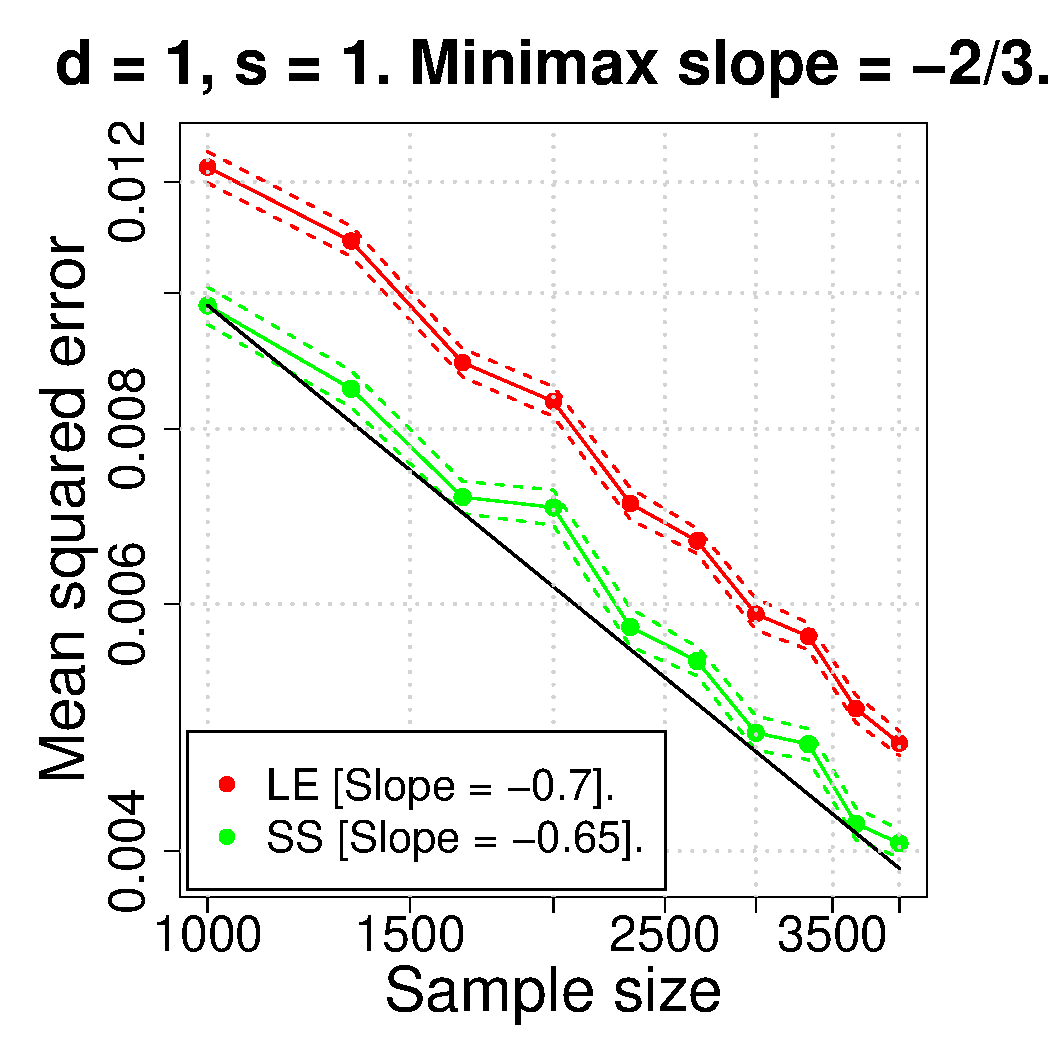
\includegraphics[width=.245\textwidth]{../figures/mse/mse_by_sample_size_1d_1s.pdf}
	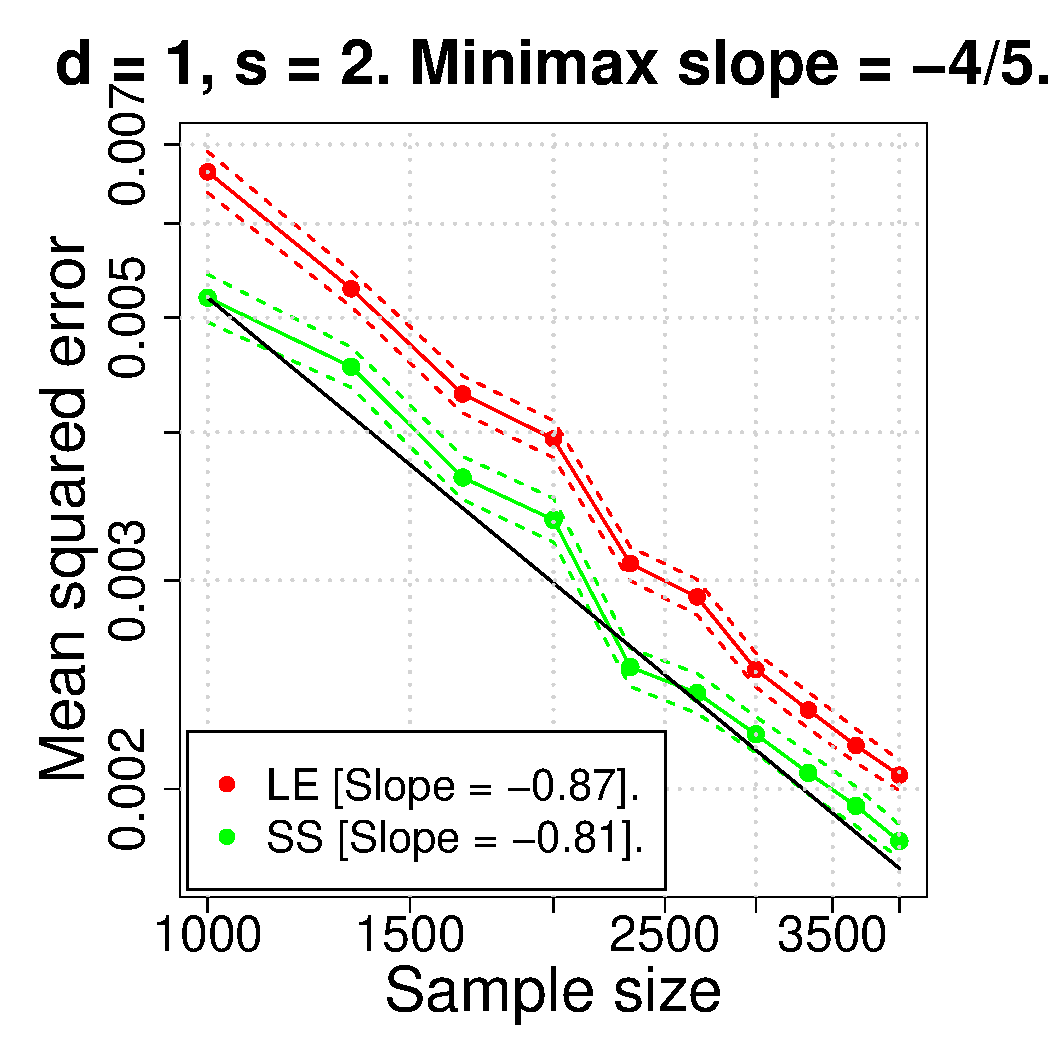
\includegraphics[width=.245\textwidth]{../figures/mse/mse_by_sample_size_1d_2s.pdf}
	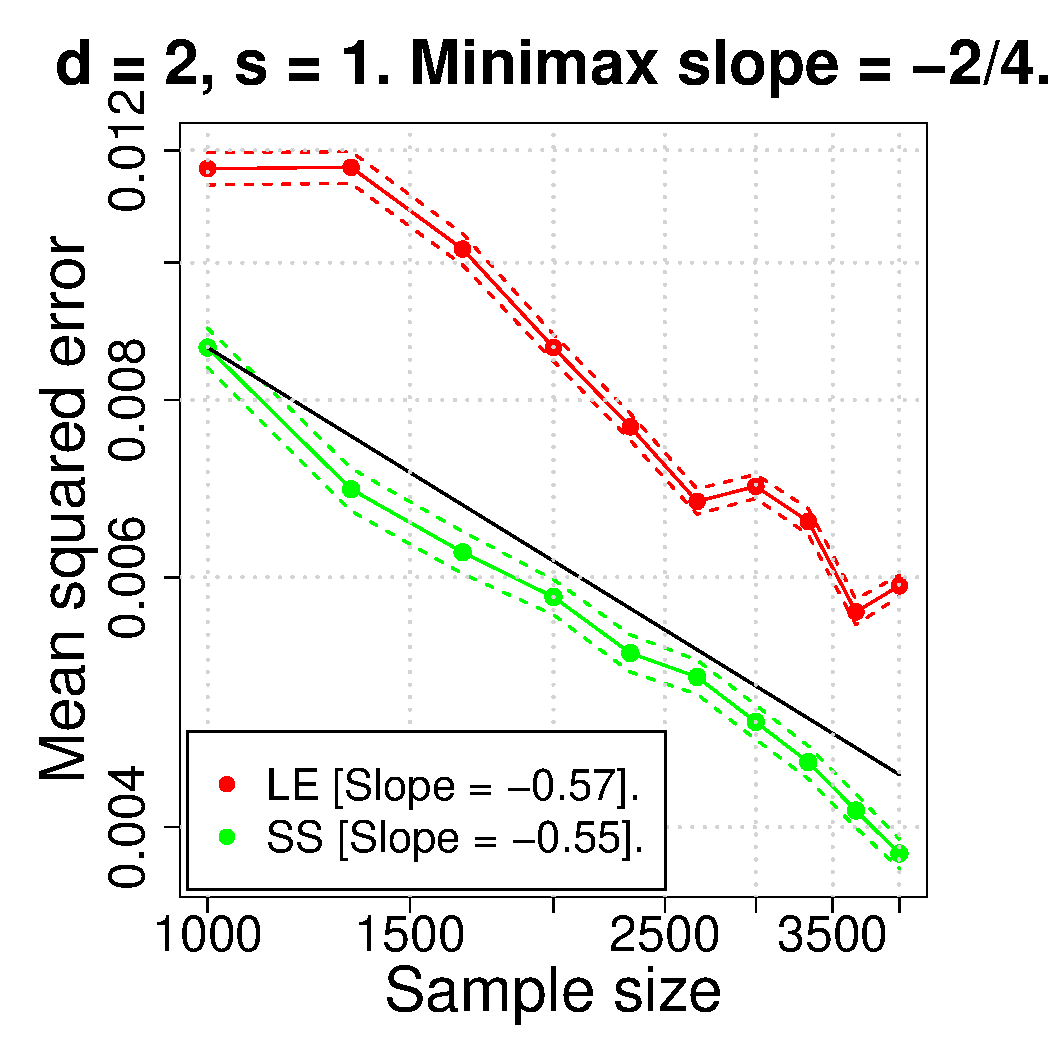
\includegraphics[width=.245\textwidth]{../figures/mse/mse_by_sample_size_2d_1s.pdf}
	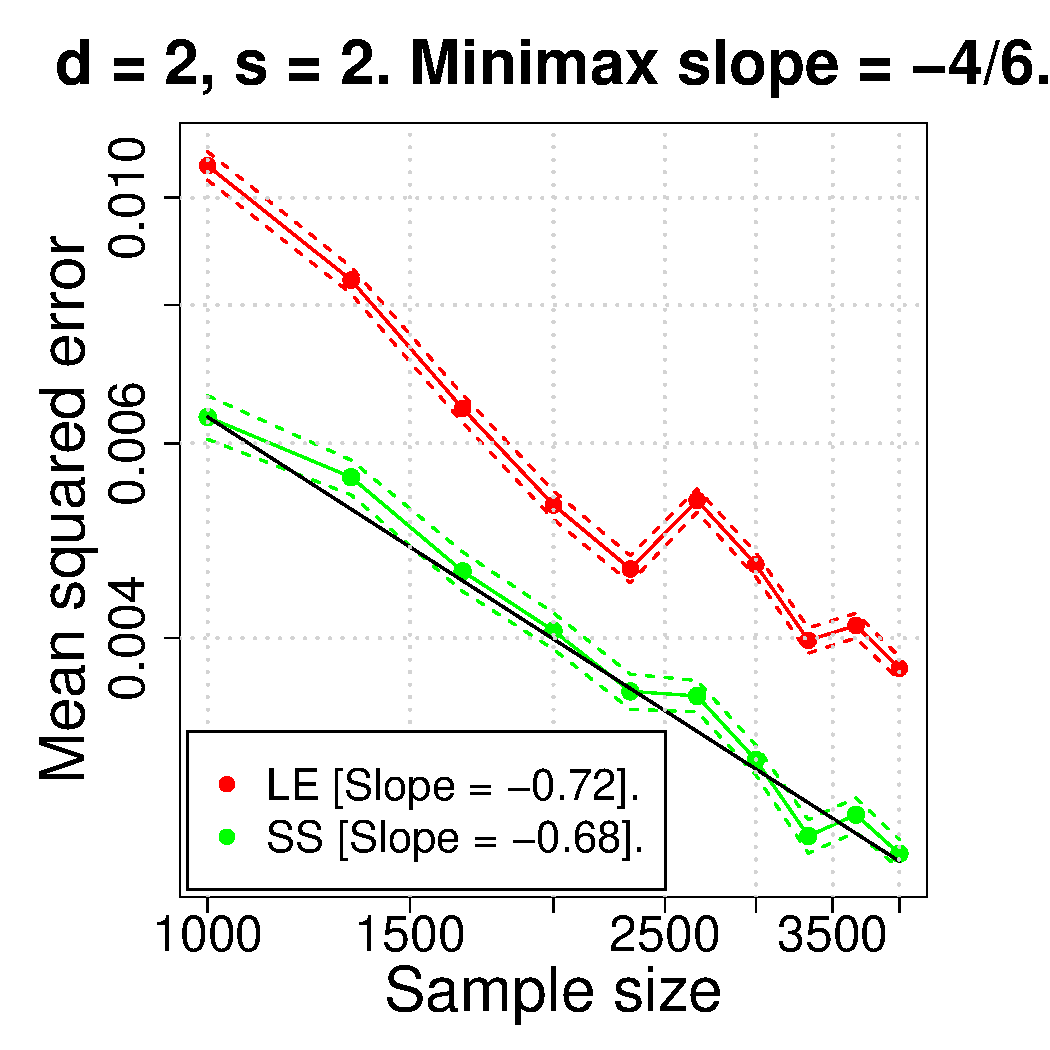
\includegraphics[width=.245\textwidth]{../figures/mse/mse_by_sample_size_2d_2s.pdf}
	\caption{In-sample mean squared error (mse) of PCR-LE (\texttt{LE}) vs. population-level spectral series (\texttt{SS}) estimator, as a function of sample size $n$. Each plot is on the log-log scale, and the results are averaged over 400 repetitions. All estimators are tuned for optimal average mse, separately at each value of $n$. The black line shows the minimax rate (in slope only; the intercept is chosen to match the observed error).}
	\label{fig:fig1}
\end{figure*}

\paragraph{Estimation.}
In our first experiment, we compare the mean-squared error of the PCR-LE estimator $\wh{f}$  to that of its population-level counterpart $\wt{f}$. We vary the sample size from $n = 1000$ to $n = 4000$; sample $n$ design points $\{X_1,\ldots,X_n\}$ from the uniform distribution on the cube $[-1,1]^d$; and sample responses $Y_i$ according to~\eqref{eqn:model} with regression function $f_0 = M/\rho_K^{s/2} \cdot \psi_K$ for $K \asymp n^{d/(2s + d)}$ (the pre-factor $M/\rho_K^{s/2}$ is chosen so that $|f_0|_{H^s(\mc{X})}^2 = M^2$). In Figure~\ref{fig:fig1} we show the in-sample mean-squared error of the two estimators as a function of $n$, for different dimensions $d$ and order of smoothness $s$. We see that both estimators have mean-squared error converging to zero at roughly the minimax rate. While the unsurprisingly population-level spectral series estimator has the smaller error, generally speaking the error of PCR-LE approaches that of the population-level spectral series method as $n$ gets larger. 

\paragraph{Testing.} 
In our second experiment, we compare the PCR-LE test $\varphi$ against the  population-level spectral series test $\wt{\varphi}$. The setup is generally the same as that of our first experiment, but to get an empirical estimate of the critical radius the details are necessarily somewhat more complicated. First we take $\mc{F} = \{M/\rho_k^{s/2} \psi_k\}_{k = 1}^{n}$ to be a discrete subset of $H^1(\mc{X};M)$. Then, for each $f_0 \in \mc{F}$, we run a given test $\phi$ (either the PCR-LE test $\phi = \varphi$, or the population-level spectral series test $\phi = \wt{\varphi}$) and record whether it was a false negative or true positive. We repeat this process over $100$ replications, giving a Monte Carlo estimate of the type II error $E_{f_0}[1 - \phi]$ for each $f_0 \in \mc{F}$. Finally, we take the smallest value of $\|f_0\|_P^2$ such $E_{f_0}[1 - \phi] \leq b$ as our estimate of the critical radius of $\phi$. 

In Figure~\ref{fig:fig2}, we see that the estimated critical radii of both the PCR-LE and population-level spectral series tests are quite close to each other, and converge at roughly the minimax rate.
\begin{figure*}[b]
	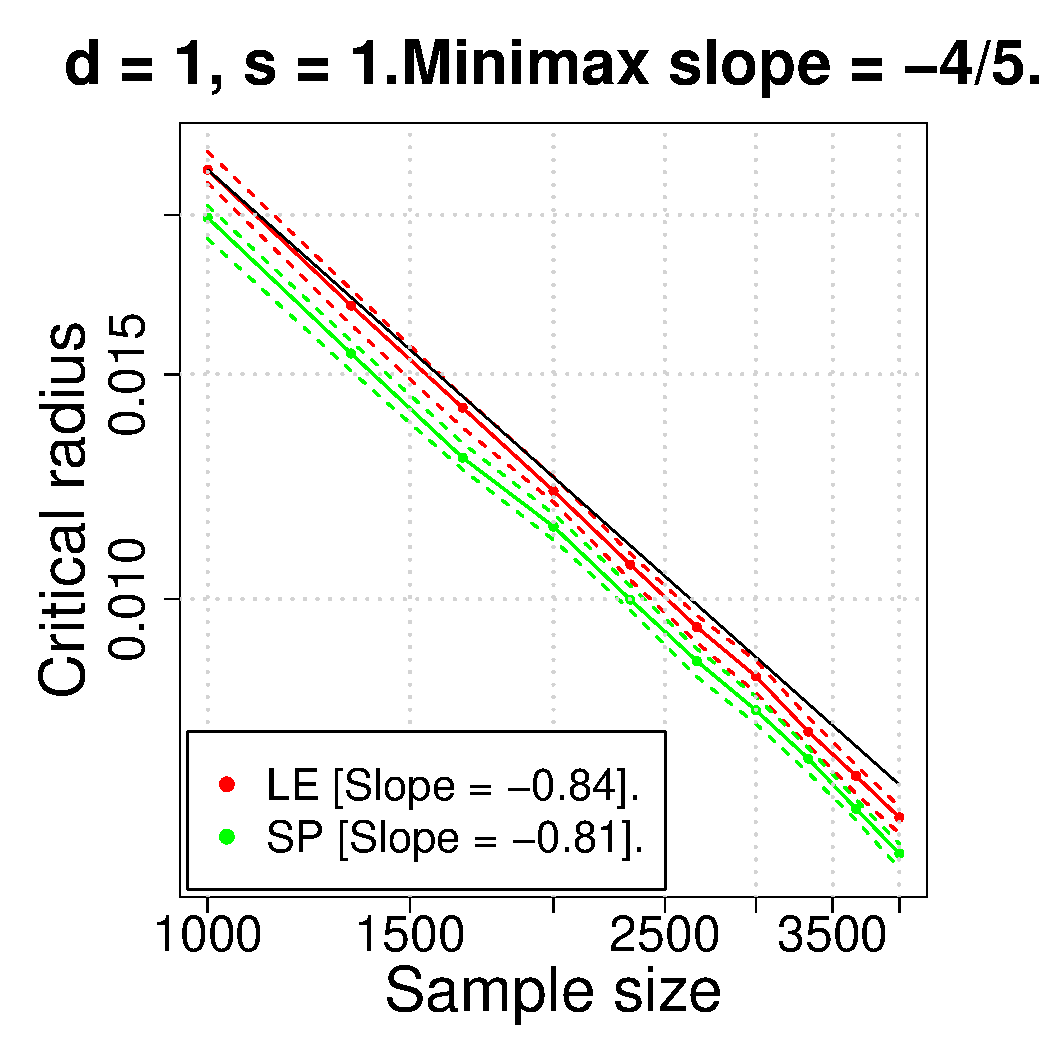
\includegraphics[width=.245\textwidth]{../figures/testing/eigenfunction/critical_radius_by_sample_size_1d_1s.pdf}
	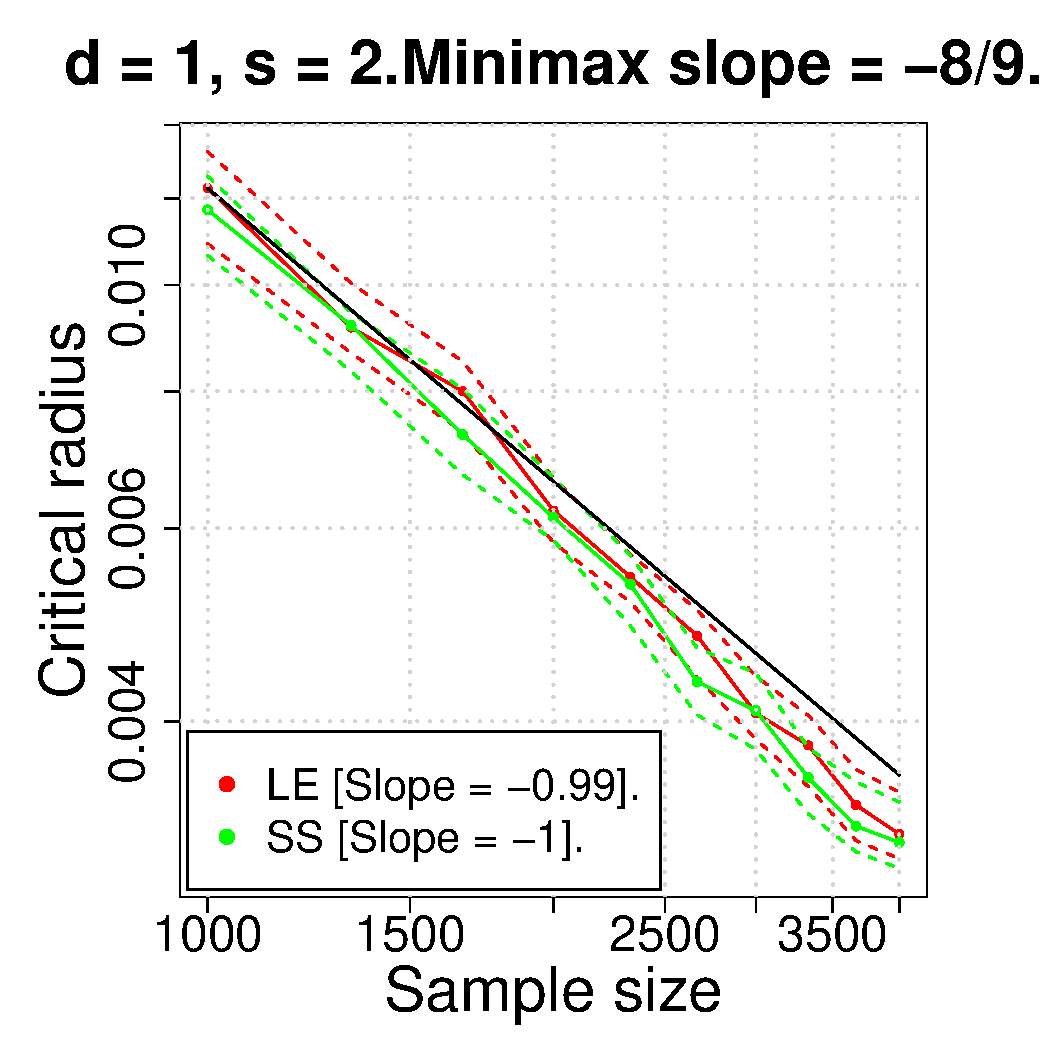
\includegraphics[width=.245\textwidth]{../figures/testing/eigenfunction/critical_radius_by_sample_size_1d_2s.pdf}
	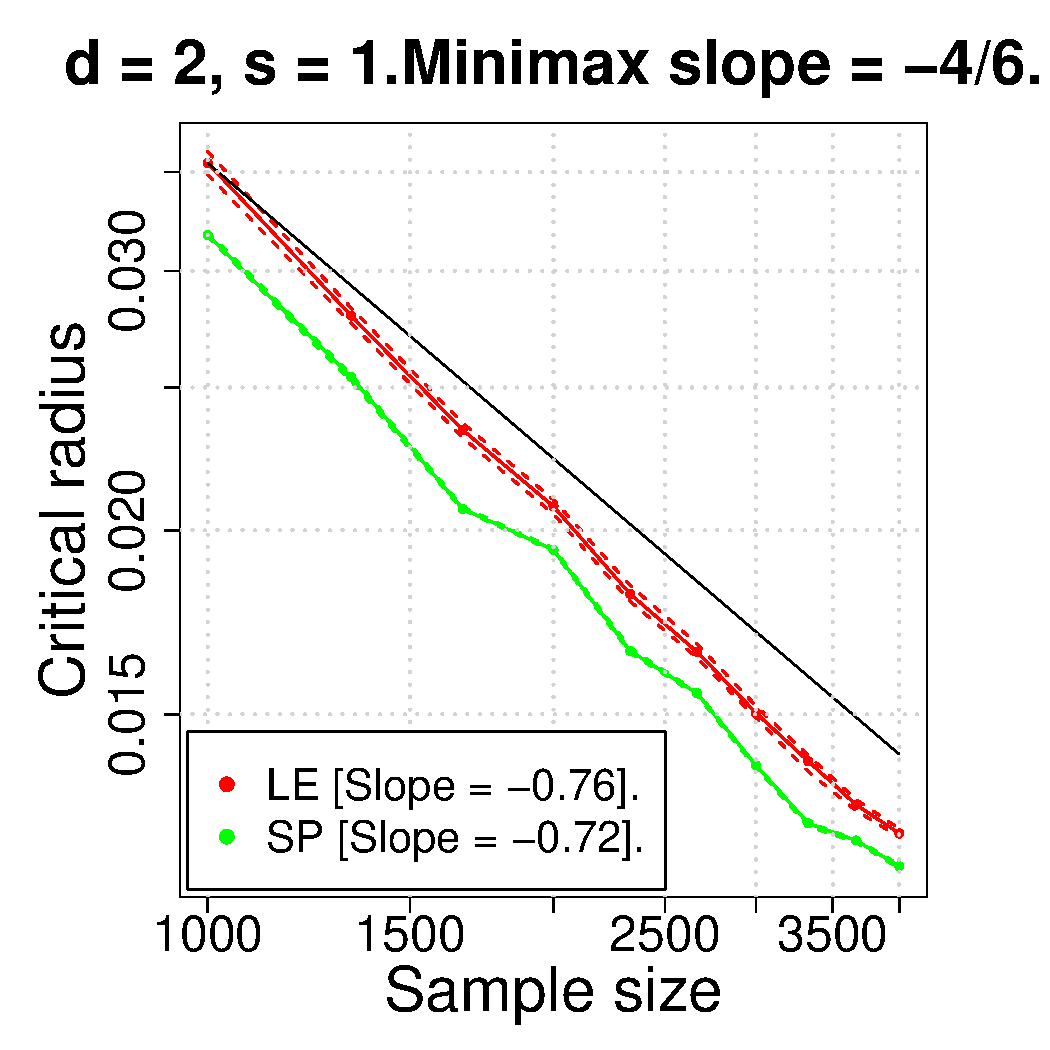
\includegraphics[width=.245\textwidth]{../figures/testing/eigenfunction/critical_radius_by_sample_size_2d_1s.pdf}
	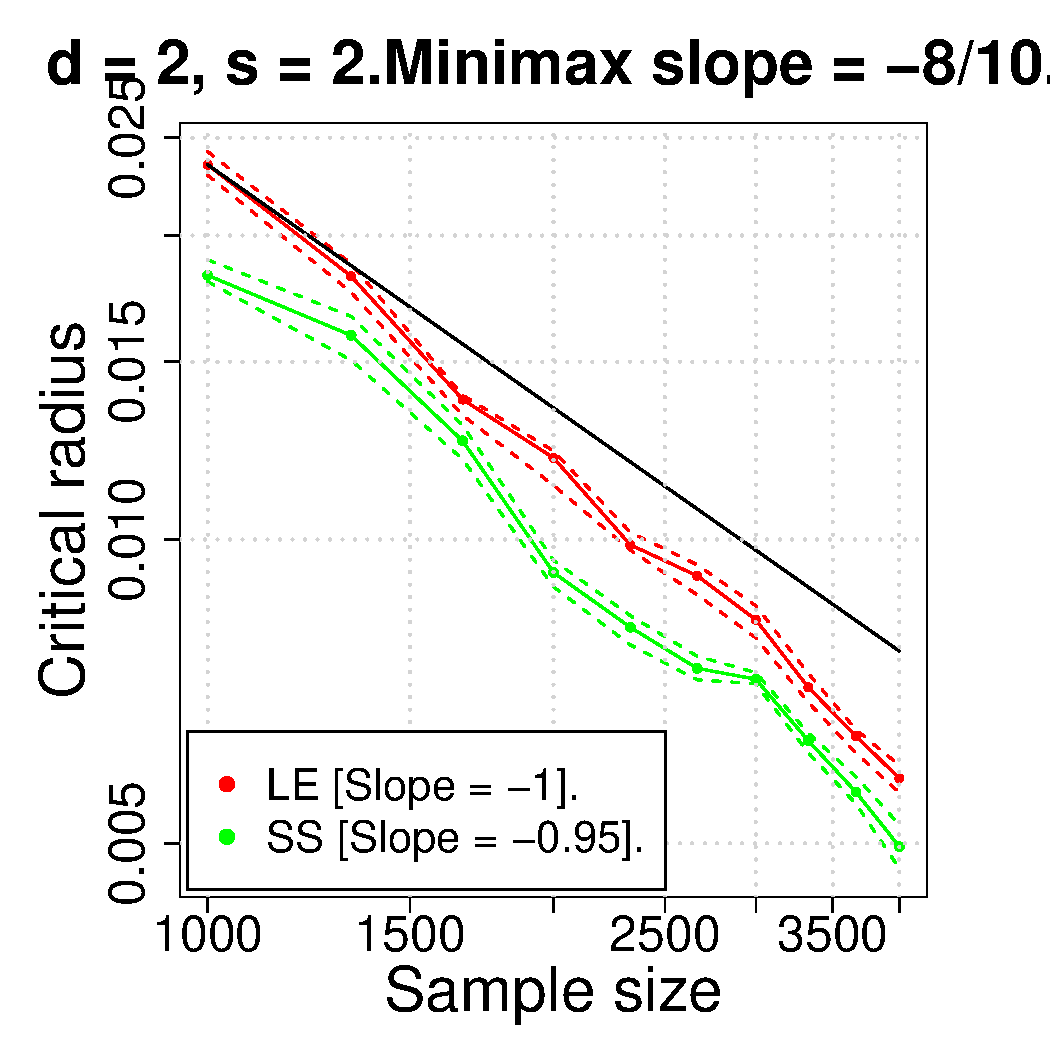
\includegraphics[width=.245\textwidth]{../figures/testing/eigenfunction/critical_radius_by_sample_size_2d_2s.pdf}
	\caption{Worst-case testing risk for PCR-LE (\texttt{LE}) and spectral series (\texttt{SP}) tests, as a function of sample size $n$. Plots are on the same scale as Figure~\ref{fig:fig1}, and black line shows the minimax rate. All tests are set to have $.05$ Type I error, and are calibrated by simulation under the null.}
	\label{fig:fig2}
\end{figure*}

\paragraph{Tuning parameters.}
Our first two experiments demonstrate that PCR-LE methods have comparable statistical performance to population-leve spectral series methods. PCR-LE depends on two tuning parameters, and in our final experiment we investigate the importance of both, focusing now on estimation. In Figure~\ref{fig:fig3}, we see how the mean-squared error of PCR-LE changes as each tuning parameter is varied. As suggested by our theory, properly choosing the number of eigenvectors $K$ is crucial: the mean-squared error curves, as a function of $K$, always have a sharply defined minimum. On the other hand, as a function of the graph radius parameter $\varepsilon$ the mean-squared error curve is much closer to flat. This squares completely with our theory, which requires that the number of eigenvectors $K$ be much more carefully tuned that the graph radius $\varepsilon$.

\begin{figure*}[tb]
	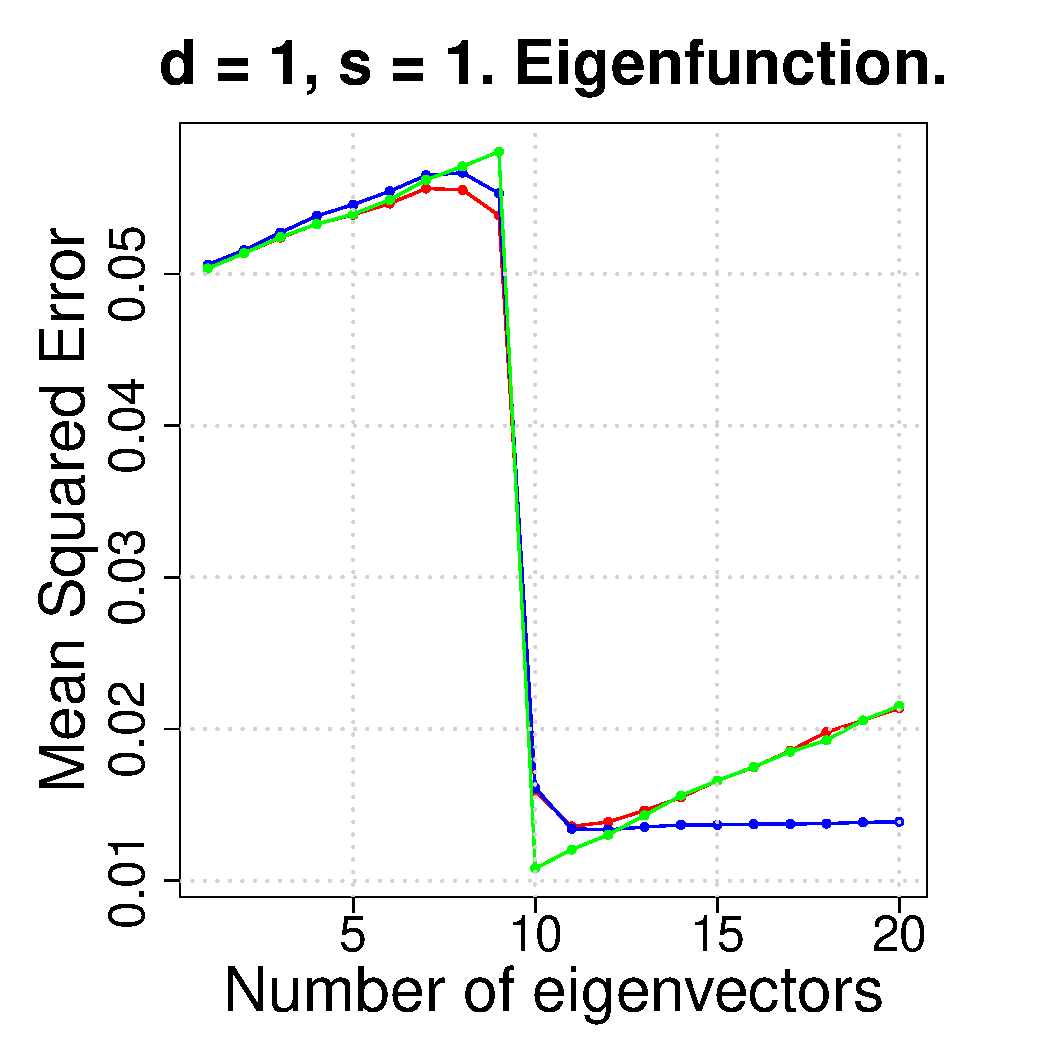
\includegraphics[width=.245\textwidth]{../figures/tuning/eigenfunction/mse_by_number_of_eigenvectors_1d_1s.pdf}
	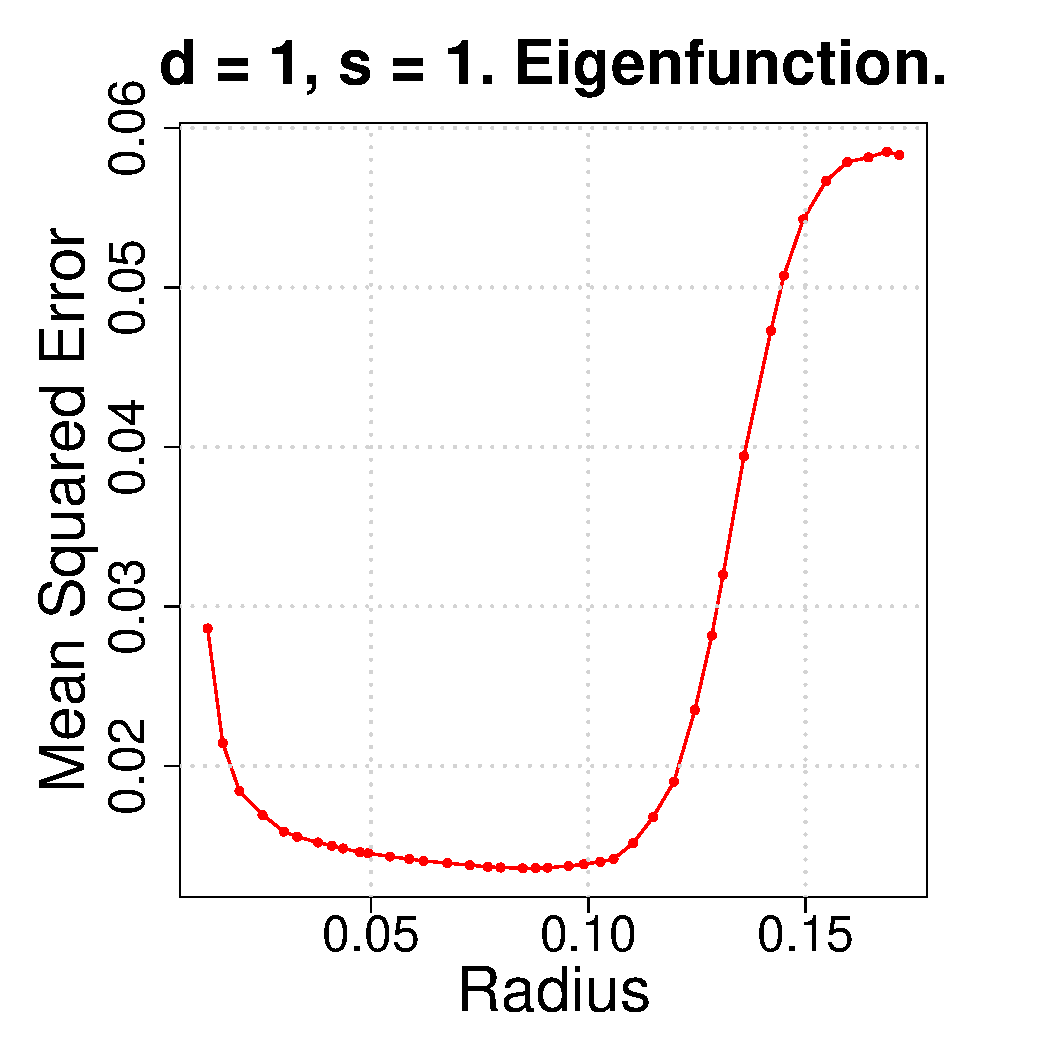
\includegraphics[width=.245\textwidth]{../figures/tuning/eigenfunction/mse_by_radius_1d_1s.pdf} 
	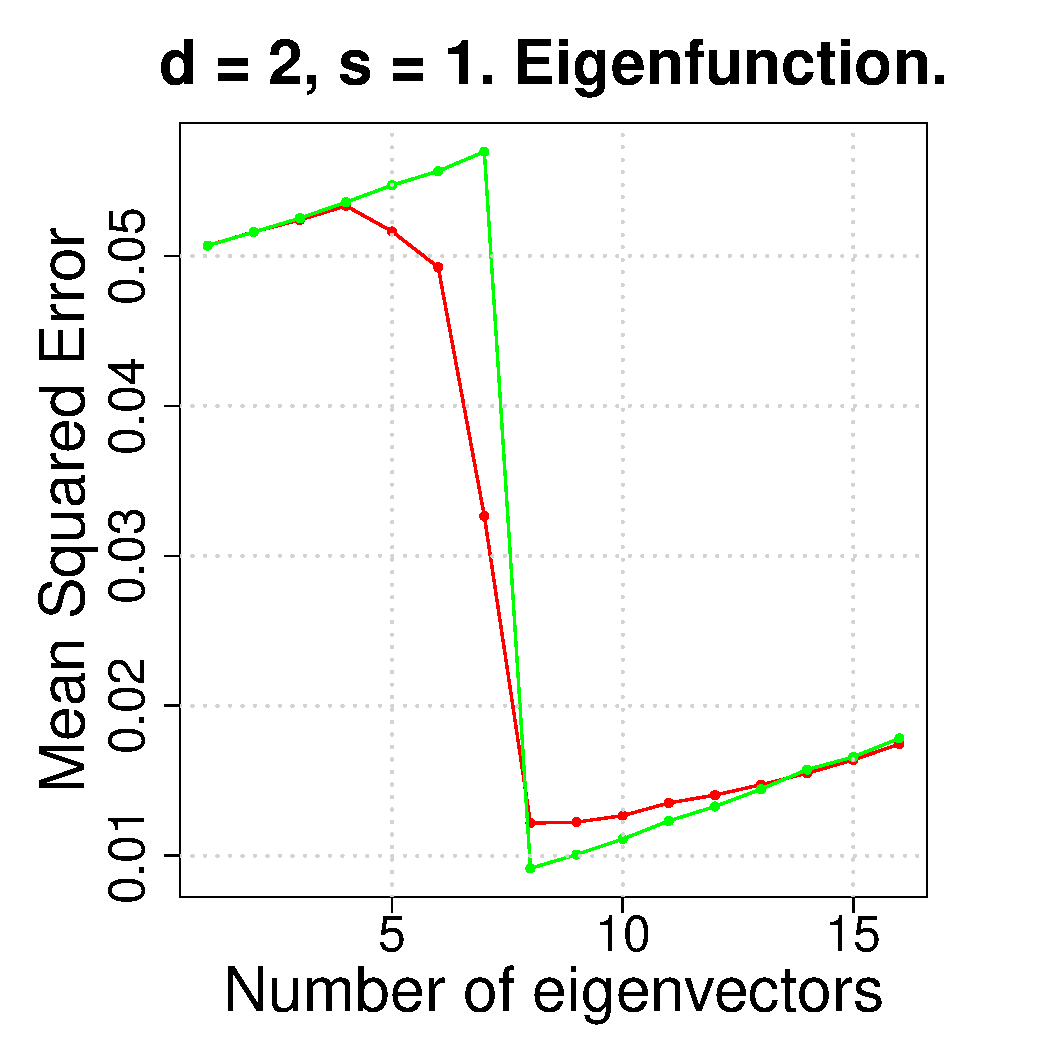
\includegraphics[width=.245\textwidth]{../figures/tuning/eigenfunction/mse_by_number_of_eigenvectors_2d_1s.pdf}
	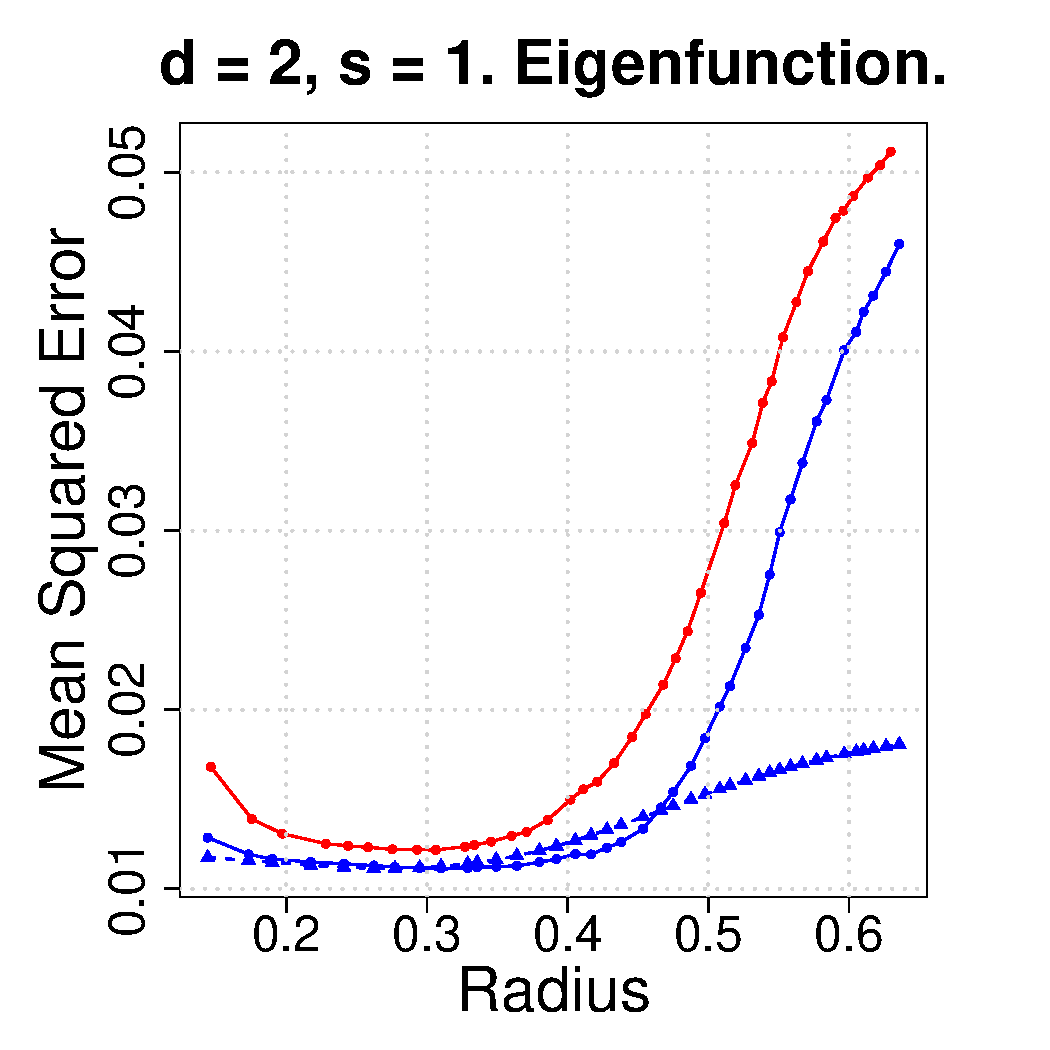
\includegraphics[width=.245\textwidth]{../figures/tuning/eigenfunction/mse_by_radius_2d_1s.pdf} 
	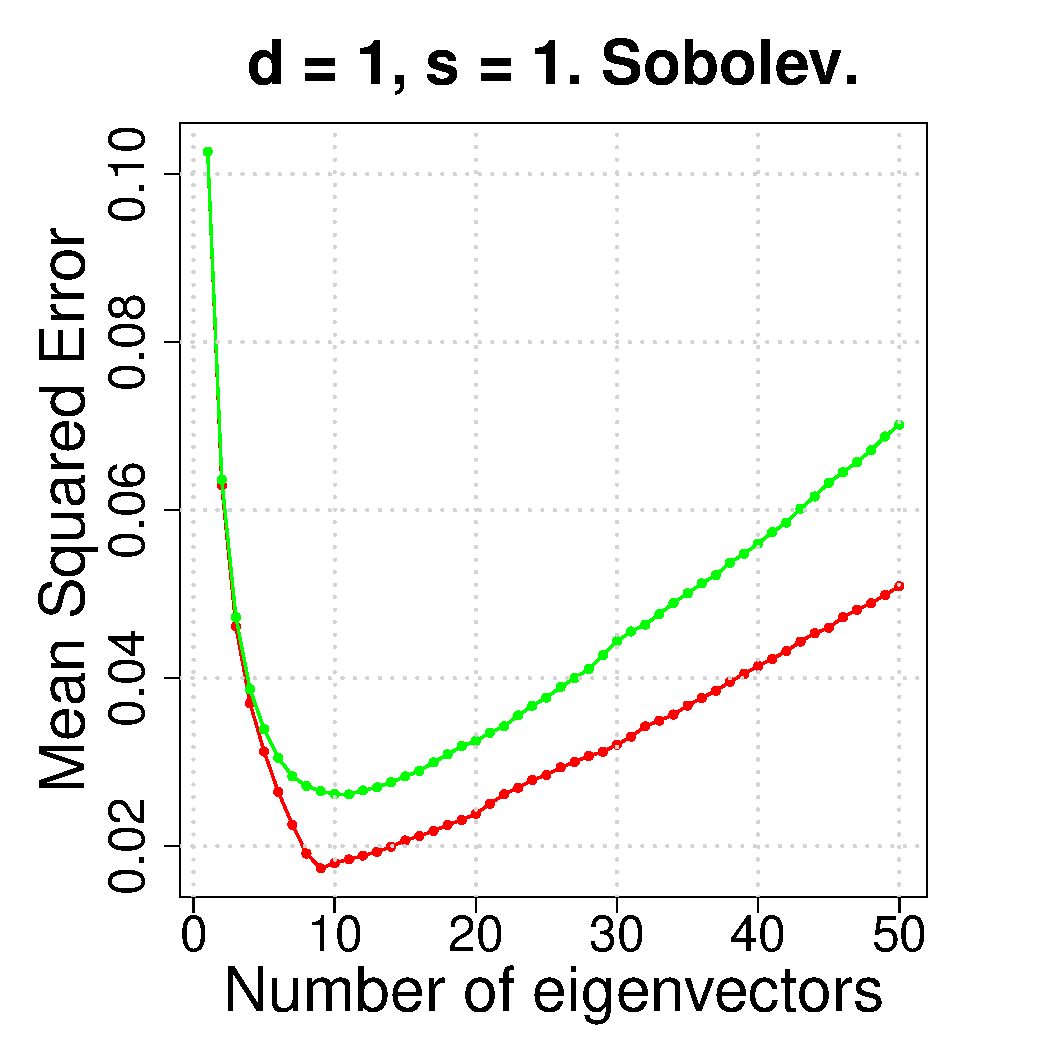
\includegraphics[width=.245\textwidth]{../figures/tuning/sobolev/mse_by_number_of_eigenvectors_1d_1s.pdf}
	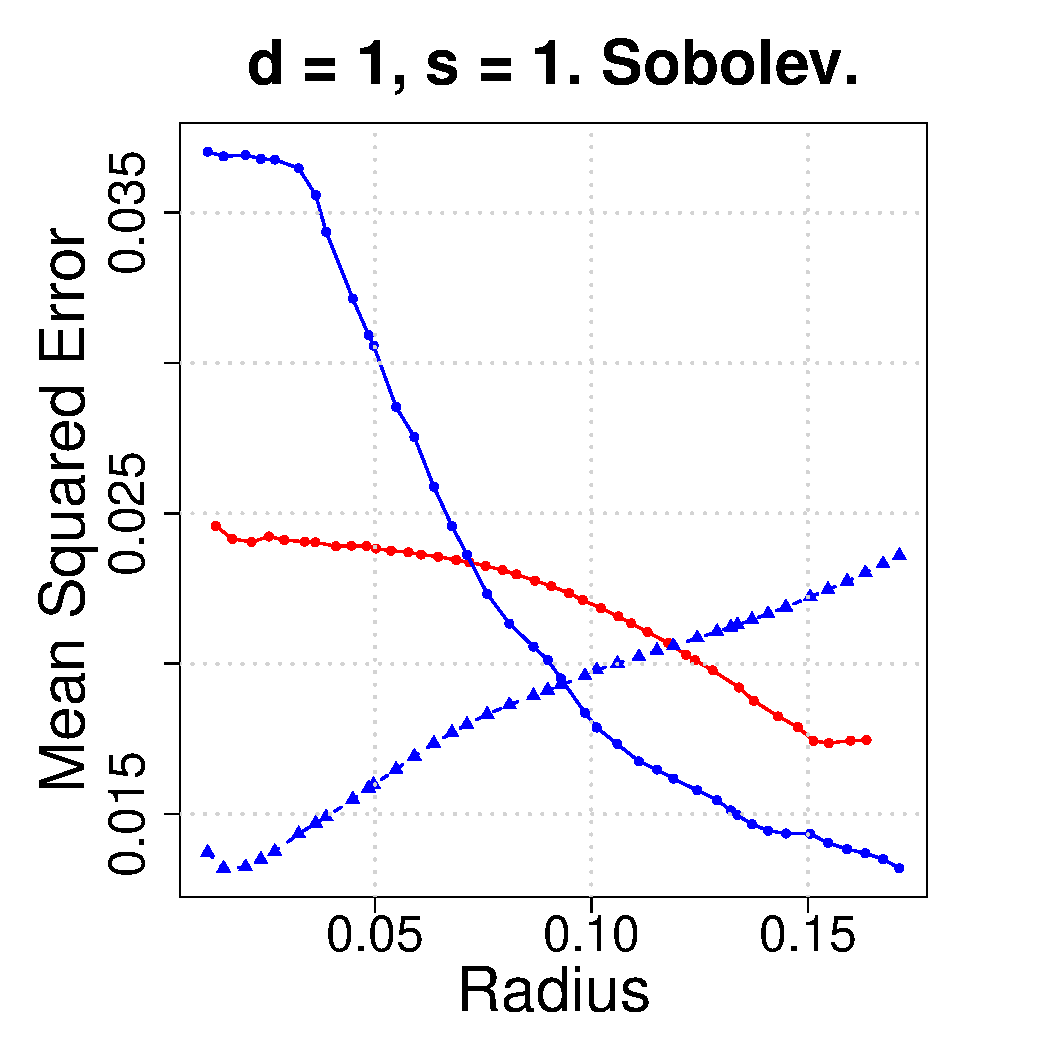
\includegraphics[width=.245\textwidth]{../figures/tuning/sobolev/mse_by_radius_1d_1s.pdf}
	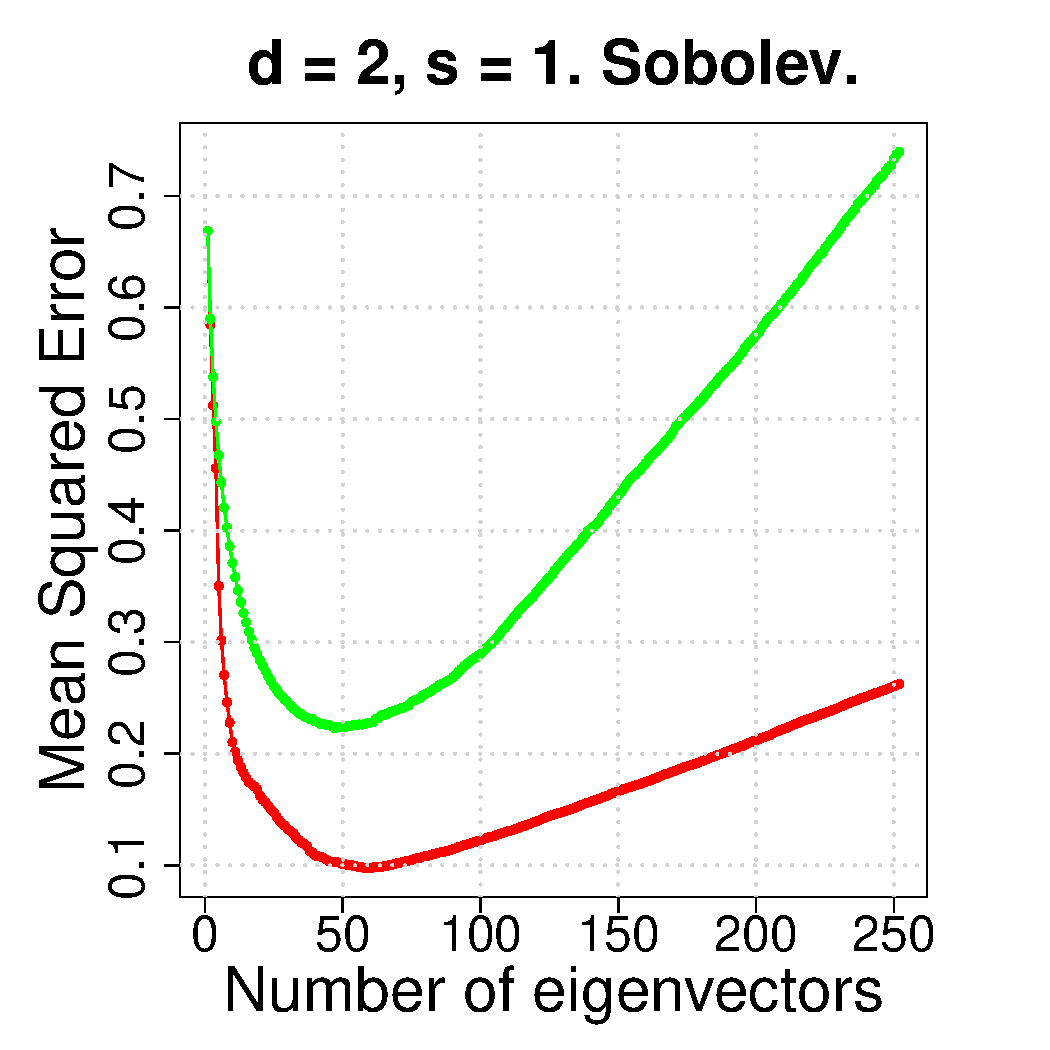
\includegraphics[width=.245\textwidth]{../figures/tuning/sobolev/mse_by_number_of_eigenvectors_2d_1s.pdf}
	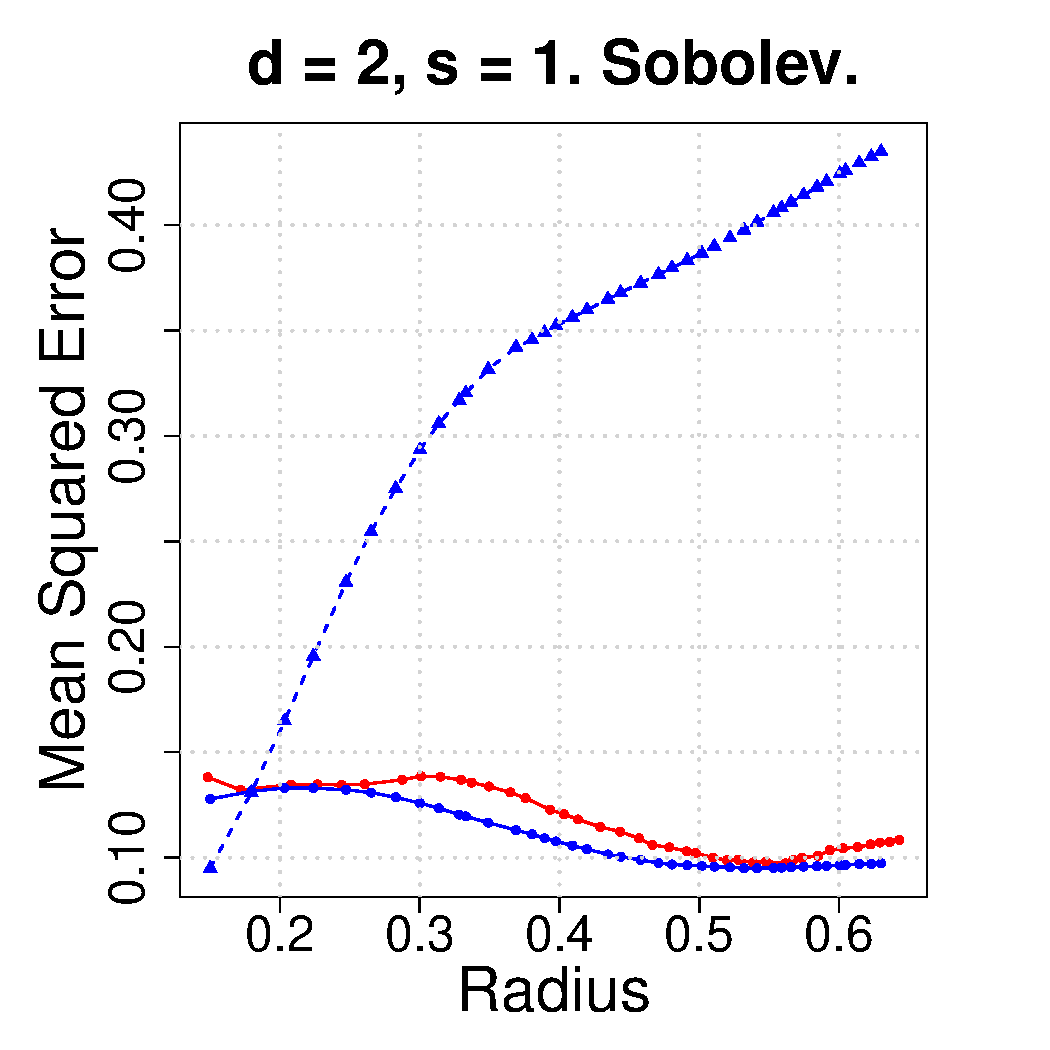
\includegraphics[width=.245\textwidth]{../figures/tuning/sobolev/mse_by_radius_2d_1s.pdf}  
	\caption{Mean squared error of PCR-LE (\textcolor{red}{red}), and population-level spectral series (\textcolor{green}{green}) estimators as a function of tuning parameters. Top row: the same regression function $f_0$ as used in Figure~\ref{fig:fig1}. Bottom row: the regression function $f_0 \propto \sum_{k} 1/\rho_k^{1/2} \psi_k$. For all experiments, the sample size $n = 1000$, and the results are averaged over $200$ repetitions. In each panel, all tuning parameters except the one being varied are set to their optimal values.}
	\label{fig:fig3}
\end{figure*}

\section{Discussion}
\label{sec:discussion}

In this work, we have derived upper bounds on the rates of convergence for regression with PCR-LE, which imply that in various settings the PCR-LE estimator and test are minimax rate-optimal over Sobolev classes. Importantly, these upper bounds hold under nonparametric conditions on the design density $p$, and allow for $p$ to be unknown and, potentially, supported on a low-dimensional manifold. Our results help explain the practical success of methods which leverage graph Laplacian eigenvectors for regression. They also distinguish such methods from more traditional spectral series procedures, which rely on a density-dependent basis and thus require the density be known a priori.

Of course, there do exist other methods for nonparametric regression which achieve optimal rates of convergence under similar (or indeed weaker) conditions on $p$. These include other graph-based approaches---graph Laplacian regularization---methods besides spectral series methods---e.g. kernel smoothing, local polynomial regression, thin-plate splines---and continuum spectral projection methods which use the eigenfunctions of an operator defined independently of $p$. To be clear, we do not advocate PCR-LE over these alternatives. Rather, we view our results as theoretically justifying a place for regression using Laplacian Eigenmaps in the nonparametric regression toolbox. 

That being said, PCR-LE does have certain advantages over each of the aforementioned approaches. We now conclude by outlining some of these advantages (limiting our discussion to estimation):
\begin{itemize}
	\item \emph{Optimality over high-dimensional Sobolev spaces}. As mentioned in the introduction, graph Laplacian regularization provably achieves minimax optimal rates over $H^1(\mc{X})$ only when $d \in \{1,2,3,4\}$ \citep{sadhanala16, green2021}; when $d \geq 5$, graph Laplacian regularization appears to be suboptimal. In contrast, PCR-LE is optimal over $H^1(\mc{X})$ for all dimensions $d$.  An even more stark contrast can be drawn between PCR-LE (and other spectral series estimators) and the first order thin-plate spline, the solution of the variational problem
	\begin{equation}
	\underset{f \in H^1(\mc{X})}{\textrm{minimize}} \quad  \|{\bf Y} - f\|_n^2 + \lambda \|f\|_{H^1(\Reals^d)}^2,
	\end{equation}
	which is optimal and indeed well-posed only when $d = 1$. This appears to be related to a general phenomenon described by~\cite{dhillon2013,dicker2017}, in which principal components analysis followed by ordinary least-squares is shown to be always competitive with, and sometimes much better than, ridge regression. 
	\item \emph{Manifold adaptivity}. An oft-recommended alternative to the population-level spectral series method considered in Section~\ref{subsec:spectral_projection} is to run OLS using eigenfunctions of a density-independent differential operator, such as the unweighted Laplacian $\Delta = \sum_{i = 1}^{d} \partial^2f/\partial x_i^2$. Under the conditions of Model~\ref{def:model_flat_euclidean}, such a method will indeed be rate-optimal, though the upper bounds may come with undesirably large constants if $p$ is very non-uniform. However, in contrast with PCR-LE, under Model~\ref{def:model_manifold} this method cannot achieve the faster minimax rates of convergence.
	\item \emph{Density adaptivity}. In Appendix~\ref{subsec:eigenmaps_beats_kernel_smoothing}, we give a simple example of a sequence of densities and regression functions $\{(p^{(n)}, f_0^{(n)}: n \in \mathbb{N}\}$ such that the expected in-sample mean squared error of PCR-LE is smaller than that of either kernel smoothing or least squares using eigenfunctions of $\Delta$. This is possible because PCR-LE induces a completely different bias than these latter two methods. In particular, when $f_0$ and $p$ satisfy the so-called \emph{cluster assumption}---meaning $f_0$ is piecewise constant in high-density regions (clusters) of $p$---then the bias of PCR-LE can be much smaller (for equivalent levels of variance) than that of kernel smoothing or least-squares with eigenfunctions of $\Delta$. 
	
	We emphasize that this does not contradict the well-known optimality properties of, for example, kernel smoothing over H\"{o}lder balls. Rather, in the standard nonparametric regression setup---which we adopt in the main part of this paper, and in which $P$ is assumed to be equivalent to Lebesgue measure---the biases of PCR-LE and kernel smoothing happen to be equivalent. But when $P$ is sufficiently non-uniform, this is no longer the case.
\end{itemize}
Grounding each of these three points on a firmer and more complete theoretical basis would be, in our view, a valuable direction for future work.

% Bibliography
\bibliographystyle{plainnat}
\bibliography{../../../graph_regression_bibliography} 

% Appendix
\appendix
\noindent 

\section{Graph-dependent error bounds}
\label{sec:fixed_graph_error_bounds}
In this section, we adopt the fixed design perspective; or equivalently, condition on $X_i = x_i$ for $i = 1,\ldots,n$. Let $G = \bigl([n],W\bigr)$ be a fixed graph on $\{1,\ldots,n\}$ with Laplacian matrix $L = \sum_{k = 1}^{n}\lambda_k v_k v_k^{\top}$; the eigenvectors have unit empirical norm, $\|v_k\|_n^2 = 1$. The randomness thus all comes from the responses 
\begin{equation}
\label{eqn:fixed_graph_regression_model}
Y_i = f_{0}(x_i) + w_i
\end{equation}
where the noise variables $w_i$ are independent $N(0,1)$. In the rest of this section, we will mildly abuse notation and write $f_0 = (f_0(x_1),\ldots,f_0(x_n)) \in \Reals^n$. We will also write ${\bf Y} = (Y_1,\ldots,Y_n)$.

\subsection{Upper bound on Estimation Error of Laplacian Eigenmaps}

\begin{lemma}
	\label{lem:fixed_graph_estimation}
	For any integer $s > 0$, and any integer $0 \leq K \leq n$, the Laplacian eigenmaps estimator $\wh{f}$ of~\eqref{eqn:laplacian_eigenmaps_estimator} satisfies
	\begin{equation}
	\label{eqn:fixed_graph_estimation}
	\|\wh{f} - f_0\|_n^2 \leq \frac{\dotp{L^sf_0}{f_0}_n}{\lambda_{K + 1}^s} + \frac{5K}{n};
	\end{equation}
	this is guaranteed if $K = 0$, and otherwise holds with probability at least $1 - \exp(-K)$ if $1 \leq K \leq n$. 
\end{lemma}
\paragraph{Proof (of Lemma~\ref{lem:fixed_graph_estimation}).}
	By the triangle inequality,
	\begin{equation}
	\label{pf:fixed_graph_estimation_1}
	\|\wh{f} - f_0\|_n^2 \leq 2\Bigl(\|\mathbb{E}\wh{f} - f_0\|_n^2 + \|\wh{f} - \mathbb{E}\wh{f}\|_n^2\Bigr).
	\end{equation}
	The first term in~\eqref{pf:fixed_graph_estimation_1} (approximation error) is non-random, since the design is fixed. The expectation $\mathbb{E}\wh{f} = \sum_{k = 1}^{K} \dotp{v_k}{f_0}_n v_k$, so that
	\begin{equation*}
	\|\mathbb{E}\wh{f} - f_0\|_n^2 = \Bigl\|\sum_{k = K + 1}^{n} \dotp{v_k}{f_0}_n v_k\Bigr\|_n^2 = \sum_{k = K + 1}^n \dotp{v_k}{f_0}_n^2.
	\end{equation*}
	In the above, the last equality relies on the fact that $v_k$ are orthonormal in $L^2(P_n)$. Using the fact that the eigenvalues are in increasing order, we obtain
	\begin{equation*}
	\sum_{k = K + 1}^n \dotp{v_k}{f_0}_n^2 \leq \frac{1}{\lambda_{K + 1}^s} \sum_{k = K + 1}^n \lambda_k^s \dotp{v_k}{f_0}_n^2 \leq \frac{\dotp{L^sf_0}{f_0}_n}{\lambda_{K + 1}^s}.
	\end{equation*}
	
	If $K = 0$, $\wh{f} = \Ebb{\wh{f}} = 0$, and the second term in~\eqref{pf:fixed_graph_estimation_1} is $0$. Otherwise the second   in~\eqref{pf:fixed_graph_estimation_1} (estimation error) is random. Observe that $\dotp{v_k}{\varepsilon}_n \overset{d}{=} Z_k/\sqrt{n}$, where $(Z_1,\ldots,Z_n) \sim N(0,I_{n \times n})$. Again using the orthonormality of the eigenvectors $v_k$, we have
	\begin{equation*}
	\|\wh{f} - \mathbb{E}\wh{f}\|_n^2 = \sum_{k = 1}^{K} \dotp{v_k}{\varepsilon}_n^2 \overset{d}{=} \frac{1}{n}\sum_{k = 1}^{K} Z_k^2.
	\end{equation*}
	Thus $\|\wh{f} - \mathbb{E}\wh{f}\|_n^2$ is equal to $1/n$ times a $\chi^2$ distribution with $K$ degrees of freedom. Consequently, it follows from a result of \citep{laurent00} that
	\begin{equation*}
	\Pbb\biggl(\|\wh{f} - \mathbb{E}\wh{f}\|_n^2 \geq \frac{K}{n} + 2\frac{\sqrt{K}}{n}\sqrt{t} + \frac{2t}{n}\biggr) \leq \exp(-t).
	\end{equation*}
	Setting $t = K$ completes the proof of the lemma.

\subsection{Upper bound on Testing Error of Laplacian Eigenmaps}

Let $\wh{T} = \sum_{k = 1}^{K} \dotp{{\bf Y}}{v_k}_n^2$, and let $\varphi = \1\{\wh{T} \geq t_a\}$. In the following Lemma, we upper bound the Type I and Type II error of the test $\varphi$.

\begin{lemma}
	\label{lem:fixed_graph_testing}
	Suppose we observe $(Y_1,x_1),\ldots,(Y_n,x_n)$ according to~\eqref{eqn:fixed_graph_regression_model}.
	\begin{itemize}
		\item If $f_0 = 0$, then $\Ebb_0[\varphi] \leq a$.
		\item Suppose $f_0 \neq 0$ satisfies
		\begin{equation}
		\label{eqn:fixed_graph_testing_critical_radius}
		\|f_0\|_n^2 \geq \frac{\dotp{L^sf_0}{f_0}_n}{\lambda_{K + 1}^s} + \frac{\sqrt{2K}}{n}\biggl[2\sqrt{\frac{1}{a}} + \sqrt{\frac{2}{b}} + \frac{32}{bn}\biggr],
		\end{equation}
		for some $s \in \mathbb{N}\setminus \{0\}$. Then $\Ebb_{f_0}[1 - \phi] \leq b$.
	\end{itemize}
\end{lemma}
\paragraph{Proof (of Lemma~\ref{lem:fixed_graph_testing}).}
We first compute the expectation and variance of $\wh{T}$, then apply Chebyshev's inequality to upper bound the Type I and Type II error.

\underline{\emph{Expectation}.}
Recall that $\wh{T} = \sum_{k = 1}^{K} \dotp{Y}{v_k}_n^2$. Expanding the square gives
\begin{equation*}
\Ebb[\wh{T}] = \sum_{k = 1}^{K} \Ebb[\dotp{Y}{v_k}_n^2] = \sum_{k = 1}^{K} \dotp{f_0}{v_k}_n^2 + \Ebb[2\dotp{f_0}{v_k}_n\dotp{\varepsilon}{v_k}_n + \dotp{\varepsilon}{v_k}_n^2] = \frac{K}{n} + \sum_{k = 1}^{K} \dotp{f_0}{v_k}_n^2.
\end{equation*}
Thus $\Ebb[\wh{T}] - t_a = \sum_{k = 1}^{K} \dotp{f_0}{v_k}_n^2 - \sqrt{2K}/n \cdot \sqrt{1/a}$. Furthermore, it is a consequence of~\eqref{eqn:fixed_graph_testing_critical_radius} that 
\begin{equation}
\label{pf:fixed_graph_testing_1}
\sum_{k = 1}^{K} \dotp{f_0}{v_k}_n^2 - \frac{\sqrt{2K}}{n}\sqrt{1/a} \geq \|f_0\|_n^2 - \frac{\dotp{L^sf_0}{f_0}_n}{\lambda_{K + 1}^s} - \frac{\sqrt{2K}}{n}\sqrt{1/a} \geq \frac{\sqrt{2K}}{n}\biggl[\sqrt{\frac{1}{a}} + \sqrt{\frac{2}{b}} + \frac{32}{bn}\biggr].
\end{equation} 

\underline{\emph{Variance}.}
Recall from the proof of Lemma~\ref{lem:fixed_graph_estimation} that $\dotp{\varepsilon}{v_k}_n \overset{d}{=} Z_k/\sqrt{n}$ for $(Z_1,\ldots,Z_n) \sim N(0,I_{n \times n})$. Expanding the square, and recalling that $\Cov[Z,Z^2] = 0$ for Gaussian random variables, we have that
\begin{equation*}
\Var\bigl[\dotp{{\bf Y}}{v_k}_n^2\bigr] = \Var\biggl[\frac{2}{n}\dotp{f_0}{v_k}_nZ_k + \frac{2}{n^2}Z_k^2\biggr] = \frac{4\dotp{f_0}{v_k}_n^2}{n} + \frac{2}{n^2}.
\end{equation*}
Moreover, since $\Cov[Z_k^2,Z_{\ell}^2] = 0$ for each $k = 1,\ldots,K$, we see that
\begin{equation*}
\Var\bigl[\wh{T}\bigr] = \sum_{k = 1}^{K} \Var\bigl[\dotp{{\bf Y}}{v_k}_n^2\bigr] = \frac{2K}{n^2} + \sum_{k = 1}^{K}\frac{4\dotp{f_0}{v_k}_n^2}{n}.
\end{equation*}

\underline{\emph{Bounds on Type I and Type II error}.}
The upper bound on Type I error follows immediately from Chebyshev's inequality. 

The upper bound on Type II error also follows from Chebyshev's inequality. We observe that~\eqref{eqn:fixed_graph_testing_critical_radius} implies $\Ebb_{f_0}[\wh{T}] = t_a$, and apply Chebyshev's inequality to deduce
\begin{equation*}
\Pbb_{f_0}\bigl(\wh{T} < t_a\bigr) \leq \Pbb_{f_0}\Bigl(|\wh{T} - \Ebb_{f_0}[\wh{T}]|^2 > |\Ebb_{f_0}[\wh{T}] - t_a|^2\Bigr) \leq \frac{\Var\bigl[\wh{T}\bigr]}{\bigl[\Ebb_{f_0}[\wh{T}] - t_a\bigr]^2} = \frac{2K/n^2 + 4/n\sum_{k = 1}^{K}\dotp{f_0}{v_k}_n^2}{\bigl[\Ebb_{f_0}[\wh{T}] - t_a\bigr]^2}.
\end{equation*}
Thus we have upper bounded the Type II error by the sum of two terms, each of which are no more than $1/(2b)$, as we now show. For the first term, after noting that~\eqref{pf:fixed_graph_testing_1} implies $\Ebb_{f_0}[\wh{T}] - t_a \geq \sqrt{2K}/n \cdot \sqrt{2/b}$, the upper bound follows:
\begin{equation*}
\frac{2K/n^2}{\bigl[\Ebb_{f_0}[\wh{T}] - t_a\bigr]^2} \leq \frac{b}{2}.
\end{equation*}
On the other hand, for the second term we use~\eqref{pf:fixed_graph_testing_1} in two ways: first to conclude that $\Ebb_{f_0}[\wh{T}] - t_a \geq 1/2 \cdot \sum_{k = 1}^{K}\dotp{f_0}{v_k}_n^2$, and second to obtain
\begin{equation*}
\frac{4\sum_{k = 1}^{K}\dotp{f_0}{v_k}_n^2}{n\bigl[\Ebb_{f_0}[\wh{T}] - t_a\bigr]^2} \leq \frac{4\sum_{k = 1}^{K}\dotp{f_0}{v_k}_n^2}{n\bigl(\sum_{k = 1}^{K}\dotp{f_0}{v_k}_n^2/2\bigr)^2} \leq \frac{16}{n\sum_{k = 1}^{K}\dotp{f_0}{v_k}_n^2} \leq \frac{b}{2}.
\end{equation*}

\section{Graph Sobolev semi-norm, flat Euclidean domain}
\label{sec:graph_quadratic_form_euclidean}
In this section we prove Proposition~\ref{prop:graph_seminorm_ho}. The proposition will follow from several intermediate results.
\begin{enumerate}
	\item~In Section~\ref{subsec:decomposition_graph_seminorm}, we show that
	\begin{equation}
	\label{pf:graph_seminorm_ho_1}
	\dotp{L_{n,\varepsilon}^sf}{f}_n \leq \frac{1}{\delta} \dotp{L_{P,\varepsilon}^sf}{f}_{P} + \frac{C\varepsilon^2}{\delta n\varepsilon^{2 + d}}M^2.
	\end{equation}
	with probability at least $1 - 2\delta$. 
	
	We term the first term on the right hand side the \emph{non-local Sobolev semi-norm}, as it is a kernelized approximation to the Sobolev semi-norm $\dotp{\Delta_P^sf}{f}_{P}$. The second term on the right hand side is a pure bias term, which as we will see is negligible compared to the non-local Sobolev semi-norm as long as $\varepsilon \ll n^{-1/(2(s -1 + d))}$. 
	\item~In Section~\ref{subsec:approximation_error_nonlocal_laplacian}, we show that when $x$ is sufficiently in the interior of $\mc{X}$, then $L_{P,\varepsilon}^kf(x)$ is a good approximation to $\Delta_P^kf(x)$, as long as $f \in H^{s}(\mc{X})$ and $p \in C^{s - 1}(\mc{X})$ for some $s \geq 2k + 1$. 
	\item~In Section~\ref{subsec:boundary_behavior_nonlocal_laplacian}, we show that when $x$ is sufficiently near the boundary of $\mc{X}$, then $L_{P,\varepsilon}^kf(x)$ is close to $0$, as long as $f \in H_0^{s}(\mc{X})$ for some $s > 2k$.
	\item~In Section~\ref{subsec:estimate_nonlocal_seminorm}, we use the results of the preceding two sections to show that if $f \in H_0^s(\mc{X};M)$ and $p \in C^{s - 1}(\mc{X})$, there exists a constant $C$ which does not depend on $f$ such that
	\begin{equation}
	\label{pf:graph_seminorm_ho_2}
	\dotp{L_{P,\varepsilon}^sf}{f}_{P} \leq CM^2.
	\end{equation}
\end{enumerate}
Finally, in Section~\ref{subsec:integrals} we provide some assorted estimates used in Sections~\ref{subsec:decomposition_graph_seminorm}. 

\paragraph{Proof (of Proposition~\ref{prop:graph_seminorm_ho}).}
Proposition~\ref{prop:graph_seminorm_ho} follows immediately from~\eqref{pf:graph_seminorm_ho_1} and~\eqref{pf:graph_seminorm_ho_2}. \qed

One note regarding notation: suppose a function $g \in H^{\ell}(U)$, where $\ell \in \mathbb{N}$ and $U$ is an open set. Let $V$ be another open set, compactly contained within $U$. Then we will use the notation $g \in H^{\ell}(V)$ to mean that the restriction $\restr{g}{V}$ of $g$ to $V$ belongs to $H^{\ell}(V)$.

\subsection{Decomposition of graph Sobolev semi-norm}
\label{subsec:decomposition_graph_seminorm}

In Lemma~\ref{lem:graph_seminorm_bias}, we decompose the graph Sobolev semi-norm (a V-statistic) into an unbiased estimate of the non-local Sobolev semi-norm (a U-statistic), and a pure bias term. We establish that the pure bias term will be small (in expectation) relative to the U-statistic whenever $\varepsilon$ is sufficiently small.
\begin{lemma}
	\label{lem:graph_seminorm_bias}
	For any $f \in L^2(\mc{X})$, the graph Sobolev semi-norm satisfies
	\begin{equation}
	\label{eqn:graph_seminorm_bias_1}
	\dotp{L_{n,\varepsilon}^sf}{f}_{n} = U_{n,\varepsilon}^{(s)}(f) + B_{n,\varepsilon}^{(s)}(f),
	\end{equation}
	such that $\mathbb{E}[U_{n,\varepsilon}^{(s)}(f)] = (n - s - 1)!/n! \cdot \dotp{L_{P,\varepsilon}^sf}{f}_P$. If additionally $f \in H^1(\mc{X};M)$ and $\varepsilon \geq n^{-1/d}$, then the bias term $B_{n,\varepsilon}^{(s)}(f)$ satisfies
	\begin{equation}
	\label{eqn:graph_seminorm_bias_2}
	\mathbb{E}\bigl[|B_{n,\varepsilon}^{(s)}(f)|\bigr] \leq \frac{C\varepsilon^2}{\delta n\varepsilon^{2 + d}}M^2.
	\end{equation}
\end{lemma}
Then~\ref{pf:graph_seminorm_ho_1} follows immediately from Lemma~\ref{lem:graph_seminorm_bias}, by Markov's inequality.
\paragraph{Proof (of Lemma~\ref{lem:graph_seminorm_bias}).}
We begin by introducing some notation. We will use bold notation $\bj = (j_1,\ldots,j_s)$ for a vector of indices where $j_i \in [n]$ for each $i$. We write $[n]^s$ for the collection of all such vectors, and $(n)^s$ for the subset of such vectors with no repeated indices. Finally, we write $D_if$ for a kernelized difference operator,
\begin{equation*}
D_if(x) := \bigl(f(x) - f(X_i)\bigr) \eta\biggl(\frac{\|X_i - x\|}{\varepsilon}\biggr),
\end{equation*}
and we let $D_{\bj}f(x) := \bigl(D_{j_1}\circ \cdots \circ D_{j_s}f\bigr)(x)$.

With this notation in hand, it is easy to represent $\dotp{L_{n,\varepsilon}^sf}{f}_{n}$ as the sum of a U-statistic and a bias term,
\begin{align*}
\dotp{L_{n,\varepsilon}^sf}{f}_{n} & = \frac{1}{n} \sum_{i = 1}^{n} L_{n,\varepsilon}^sf(X_i) \cdot f(X_i) \\
& = \underbrace{\frac{1}{n^{s + 1}\varepsilon^{s(d + 2)}} \sum_{{i\bf j} \in (n)^{s + 1}}D_{\bj}f(X_i) \cdot f(X_i)}_{=:U_{n,\varepsilon}^{(s)}(f)} + \underbrace{\frac{1}{n^{s + 1}\varepsilon^{s(d + 2)}} \sum_{\substack{i\bj \in \\ [n]^{s + 1}\setminus (n)^{s + 1}}} D_{\bj}f(X_i) \cdot f(X_i)}_{=:B_{n,\varepsilon}^{(s)}(f)}
\end{align*}
When the indices of $i\bj$ are all distinct, it follows straightforwardly from the law of iterated expectation that
\begin{equation*}
\mathbb{E}[ D_{\bj}f(X_i) \cdot f(X_i)] = \varepsilon^{s(d + 2)}\mathbb{E}[L_{P,\varepsilon}^sf(X_i) \cdot f(X_i)] = \dotp{L_{P,\varepsilon}^sf}{f}_{P}, 
\end{equation*}
which in turn implies $\mathbb{E}[U_{n,\varepsilon}^{(s)}(f)] = (n - s - 1)!/n! \cdot \dotp{L_{P,\varepsilon}^sf}{f}_P$. 

It remains to show~\eqref{eqn:graph_seminorm_bias_2}. By adding and subtracting $f(X_{\bj_1})$, we obtain by symmetry that
\begin{equation*}
\sum_{\substack{i\bj \in \\ [n]^{s + 1}\setminus (n)^{s + 1}}} D_{\bj}f(X_i) \cdot f(X_i) = \frac{1}{2} \cdot \sum_{\substack{i\bj \in \\ [n]^{s + 1}\setminus (n)^{s + 1}}} D_{\bj}f(X_i) \cdot \bigl(f(X_i) - f(X_{\bj_1})\bigr),
\end{equation*}
and consequently
\begin{equation*}
\Ebb\Bigl[\sum_{\substack{i\bj \in \\ [n]^{s + 1}\setminus (n)^{s + 1}}} D_{\bj}f(X_i) \cdot f(X_i)\Bigr] \leq \frac{1}{2} \cdot \sum_{\substack{i\bj \in \\ [n]^{s + 1}\setminus (n)^{s + 1}}} \Ebb\Bigl[\bigl|D_{\bj}f(X_i)\bigr| \cdot \bigl|f(X_i) - f(X_{\bj_1})\bigr|\Bigr].
\end{equation*}
In Lemma~\ref{lem:graph_seminorm_bias2}, we show that if $f \in H^1(\mc{X};M)$, then for any $i\bj \in [n]^{s + 1}$ which contains a total of $k + 1$ distinct indices, 
\begin{equation*}
\Ebb\Bigl[\bigl|D_{\bj}f(X_i)\bigr| \cdot \bigl|f(X_i) - f(X_{\bj_1})\bigr|\Bigr] \leq C_1 \varepsilon^{2 + kd} M^2.
\end{equation*}
This shows us that the expectation of $|B_{n,\varepsilon}^s(f)|$ can bounded from above by the sum over several different terms, as follows:
\begin{align*}
\Ebb\Bigl[|B_{n,\varepsilon}^s(f)|\Bigr] & \leq C_1\frac{\varepsilon^2}{n\varepsilon^{2s}}M^2 \sum_{\substack{i\bj \in \\ [n]^{s + 1}\setminus (n)^{s + 1}}} \frac{1}{(n\varepsilon^d)^s}  \varepsilon^{(|i\bj| - 1)d} \\
& \leq C_1\frac{\varepsilon^2}{n\varepsilon^{2s}}M^2  \sum_{k = 1}^{s - 1} \frac{(n\varepsilon^d)^k}{(n\varepsilon^d)^s}n.
\end{align*}
Finally, we note that by assumption $n\varepsilon^d \geq 1$, so that in the above sum the factor of $(n\varepsilon^d)^k$ is largest when $k = s- 1$. We conclude that
\begin{equation*}
\Ebb\Bigl[|B_{n,\varepsilon}^s(f)|\Bigr] \leq C_1 (s - 1) \frac{\varepsilon^2}{n\varepsilon^{2s + d}}M^2,
\end{equation*}
which is the desired result.

\subsection{Approximation error of non-local Laplacian}
\label{subsec:approximation_error_nonlocal_laplacian}

In this section, we establish the convergence $L_{P,\varepsilon}^kf \to \sigma_{\eta}^k\Delta_P^kf$ as $\varepsilon \to 0$. More precisely, we give an upper bound on the squared difference between $L_{P,\varepsilon}^kf$ and  $\sigma_{\eta}^k\Delta_P^kf$ as a function of $\varepsilon$. The bound holds for all $x \in \mc{X}_{k\varepsilon}$, and $f \in H^{s}(\mc{X})$, as long as $s \geq 2k + 1$.  \textcolor{red}{(TODO): Make sure that $\sigma_{\eta}$ is defined somewhere.}
\begin{lemma}
	\label{lem:approximation_error_nonlocal_laplacian}
	Assume Model~\ref{def:model_flat_euclidean}. Let $s \in \mathbb{N} \setminus \{0,1\}$, suppose that $f \in H^s(\mc{X};M)$, and if $s > 1$ suppose that $p \in C^{s - 1}(\mc{X})$. Let $L_{P,\varepsilon}$ be define with respect to a kernel $\eta$ that satisfies~\ref{asmp:kernel_flat_euclidean}. Then there exist constants $C_1$ and $C_2$ that do not depend on $f$, such that each of the following statements hold.
	\begin{itemize}
		\item If $s$ is odd and $k = (s - 1)/2$, then
		\begin{equation}
		\label{eqn:approximation_error_nonlocal_laplacian_1}
		\|L_{P,\varepsilon}^kf - \Delta_P^kf\|_{L^2(\mc{X}_{k\varepsilon})} \leq C_1 M \varepsilon
		\end{equation}
		\item If $s$ is even and $k = (s - 2)/2$, then
		\begin{equation}
		\label{eqn:approximation_error_nonlocal_laplacian_2}
		\|L_{P,\varepsilon}^kf - \Delta_P^kf\|_{L^2(\mc{X}_{k\varepsilon})} \leq C_2 M \varepsilon^2.
		\end{equation}
	\end{itemize}
\end{lemma}
We remark that when $k = 1$ and $f \in C^3(\mc{X})$ or $C^4(\mc{X})$, statements of this kind are well known \textcolor{red}{(references)}, and indeed stronger results---with $L^{\infty}(\mc{X})$ norm replacing $L^2(\mc{X})$ norm---hold. When dealing with the iterated Laplacian, and functions $f$ which are regular only in the Sobolev sense, the proof is somewhat more lengthy, but the spirit of the result is largely the same.
 
\paragraph{Proof (of Lemma~\ref{lem:approximation_error_nonlocal_laplacian}).}
Throughout this proof, we shall assume that $f$ and $p$ are smooth functions, meaning they belong to $C^{\infty}(\mc{X})$. This is without loss of generality, since $C^{\infty}(\mc{X})$ is dense in both $H^s(\mc{X})$ and $C^{s - 1}(\mc{X})$, and since both sides of the inequalities~\eqref{eqn:approximation_error_nonlocal_laplacian_1} and~\eqref{eqn:approximation_error_nonlocal_laplacian_2} are continuous with respect to $\|\cdot\|_{H^s(\mc{X})}$ and $\|\cdot\|_{C^{s - 1}(\mc{X})}$ norms.

We will actually prove a more general set of statements than contained in Lemma~\ref{lem:approximation_error_nonlocal_laplacian}, more general in the sense that they give estimates for all $k$, rather than simply the particular choices of $k$ given above. In particular, we will prove that the following two statements hold for any $s \in \mathbb{N}$ and any $k \in \mathbb{N} \setminus \{0\}$. 
\begin{itemize}
	\item If $k \geq s/2$, then for every $x \in \mc{X}_{k\varepsilon}$, 
	\begin{equation}
	\label{pf:approximation_error_nonlocal_laplacian_0}
	L_{P,\varepsilon}^kf(x) = g_s(x) \varepsilon^{s - 2k}
	\end{equation}
	for a function $g_s$ that satisfies
	\begin{equation}
	\label{pf:approximation_error_nonlocal_laplacian_0.5}
	\|g_s\|_{L^2(\mc{X}_{k\varepsilon})} \leq C \|p\|_{C^{q}(\mc{X})}^k M 
	\end{equation}
	where $q = 1$ if $s =0$ or $s = 1$, and otherwise $q = s - 1$. 
	\item If $k < s/2$, then for every $x \in \mc{X}_{k\varepsilon}$,
	\begin{equation}
	\label{pf:approximation_error_nonlocal_laplacian_1}
	L_{P,\varepsilon}^kf(x) = \sigma_{\eta}^k \cdot \Delta_{P}^kf(x) + \sum_{j = 1}^{\floor{(s - 1)/2} - k} g_{2(j + k)}(x)\varepsilon^{2j} + g_{s}(x) \varepsilon^{s - 2k}.
	\end{equation}
	for functions $g_j$ that satisfy
	\begin{equation}
	\label{pf:approximation_error_nonlocal_laplacian_1.5}
	\|g_j\|_{H^{s - j}(\mc{X}_{k\varepsilon})} \leq C \|p\|_{C^{s - 1}(\mc{X})}^k M.
	\end{equation}
\end{itemize}
In the statement above, recall that $H^0(\mc{X}_{k\varepsilon}) = L^2(\mc{X}_{k\varepsilon})$. Additionally, note that we may speak of the pointwise behavior of derivatives of $f$ because we have assumed that $f$ is a smooth function. Observe that~\eqref{eqn:approximation_error_nonlocal_laplacian_1} follows upon taking $k = \floor{(s - 1)/2}$ in~\eqref{pf:approximation_error_nonlocal_laplacian_1}, whence we have
\begin{equation*}
\bigl(L_{P,\varepsilon}^kf(x) - \sigma_{\eta}^k \Delta_{P}^kf(x)\bigr)^2 = \varepsilon^2 \bigl(g_s(x)\bigr)^2
\end{equation*}
for some $g_s \in \Leb^2(\mc{X}_{k\varepsilon},C \cdot M \cdot \|p\|_{C^{s - 1}(\mc{X})})$, and integrating over $\mc{X}_{k\varepsilon}$ gives the desired result. \eqref{eqn:approximation_error_nonlocal_laplacian_2} follows from~\eqref{pf:approximation_error_nonlocal_laplacian_1} in an identical fashion. 

It thus remains establish~\eqref{pf:approximation_error_nonlocal_laplacian_1}, and~\eqref{pf:approximation_error_nonlocal_laplacian_0} which is an important part of proving~\eqref{pf:approximation_error_nonlocal_laplacian_1}. We will do so by induction on $k$. Note that throughout, we will let $g_j$ refer to functions which may change from line to line, but which always satisfy~\eqref{pf:approximation_error_nonlocal_laplacian_1.5}. 

\underline{\textit{Proof of~\eqref{pf:approximation_error_nonlocal_laplacian_0} and~\eqref{pf:approximation_error_nonlocal_laplacian_1}, base case.}}

We begin with the base case, where $k = 1$. Again, we point out that although desired result is known when $s = 3$ or $s = 4$, and $f$ is regular in the H\"{o}lder sense, we require estimates for all $s \in \mathbb{N}$ when $f$ is regular in the Sobolev sense.

When $s = 0$, the inequality~\eqref{pf:approximation_error_nonlocal_laplacian_0} is implied by Lemma~\ref{lem:l2estimate_nonlocal_laplacian}.  When $s \geq 1$, we proceed using Taylor expansion. For any $x \in \mc{X}_{\varepsilon}$, we have that $B(x,\varepsilon) \subseteq \mc{X}$. Thus for any $x' \in B(x,\varepsilon)$, we may take an order $s$ Taylor expansion of $f$ around $x' = x$, and an order $q$ Taylor expansion of $p$ around $x' = x$, where $q = 1$ if $s = 1$, and otherwise $q = s - 1$. (See Section~\ref{subsec:taylor_expansion} for a review of the notation we use for Taylor expansions, as well as some properties that we make use of shortly.) This allows us to express $L_{P,\varepsilon}f(x)$ as the sum of three terms,
\begin{align*}
L_{P,\varepsilon}f(x) & = \frac{1}{\varepsilon^{d + 2}}\sum_{j_1 = 1}^{s - 1} \sum_{j_2 = 0}^{q - 1}\frac{1}{j_1!j_2!}  \int_{\mc{X}} \bigl(d_x^{j_1}f\bigr)(x' - x) \bigl(d_x^{j_2}p\bigr)(x' - x) \eta\biggl(\frac{\|x' - x\|}{\varepsilon}\biggr) \,dx' \quad + \\
& \quad \frac{1}{\varepsilon^{d + 2}}\sum_{j = 1}^{s - 1} \frac{1}{j!} \int_{\mc{X}} \bigl(d_x^jf\bigr)(x' - x)  r_{x'}^{q}(x;p) \eta\biggl(\frac{\|x' - x\|}{\varepsilon}\biggr) \,dx' \quad  + \\
& \quad \frac{1}{\varepsilon^{d + 2}} \int_{\mc{X}} r_{x'}^j(x;f) \eta\biggl(\frac{\|x' - x\|}{\varepsilon}\biggr) \,dP(x').
\end{align*}
Here we have adopted the convention that $\sum_{j = 1}^{0} = 0$. 

Changing variables to $z = (x' - x)/\varepsilon$, we can rewrite the above expression as 
\begin{align*}
L_{P,\varepsilon}f(x) & = \frac{1}{\varepsilon^{2}}\sum_{j_1 = 1}^{s - 1} \sum_{j_2 = 0}^{q - 1}\frac{\varepsilon^{j_1 + j_2}}{j_1!j_2!}  \int d_x^{j_1}f(z) d_x^{j_2}p(z) \eta\bigl(\|z\|\bigr) \,dz \quad + \\
& \quad \frac{1}{\varepsilon^{2}} \sum_{j = 1}^{s - 1} \frac{\varepsilon^j}{j!} \int d_x^jf(z)  r_{zh + x}^{q}(x;p) \eta\bigl(\|z\|\bigr) \,dz \quad  + \\
& \quad \frac{1}{\varepsilon^{2}} \int r_{zh + x}^j(x;f) \eta\bigl(\|z\|\bigr) p(zh + x)\,dz \\
& := G_1(x) + G_2(x) + G_3(x).
\end{align*}
We now separately consider each of $G_1(x),G_2(x)$ and $G_3(x)$. We will establish that if $s = 1$ or $s = 2$, then $G_1(x) = 0$, and otherwise if $s \geq 3$ that
\begin{equation*}
G_1(x) = \sigma_{\eta}\Delta_Pf(x) + \sum_{j = 1}^{\floor{(s - 1)/2} - 1}g_{2(j + 1)}(x)\varepsilon^{2j} + g_{s}(x)\varepsilon^{s - 2}.
\end{equation*}
On the other hand, we will establish that if $s = 1$ then $G_2(x) = 0$, and otherwise for $s \geq 2$
\begin{equation}
\label{pf:approximation_error_nonlocal_laplacian_2}
\|G_2\|_{\Leb^2(\mc{X}_{\varepsilon})} \leq C \varepsilon^{s - 2} M \|p\|_{C^{s - 1}(\mc{X})};
\end{equation}
this same estimate will hold for $G_3$ for all $s \geq 1$. Together these will imply~\eqref{pf:approximation_error_nonlocal_laplacian_0} and~\eqref{pf:approximation_error_nonlocal_laplacian_1}. 

\emph{Estimate on $G_1(x)$.}
If $s = 1$, then $s - 1 = 0$, and so $G_1(x) = 0$. We may therefore suppose $s \geq 2$. Recall that
\begin{equation}
G_1(x) = \sum_{j_1 = 1}^{s - 1} \sum_{j_2 = 0}^{q - 1} \frac{\varepsilon^{j_1 + j_2 - 2}}{j_1!j_2!}  \underbrace{\int_{B(0,1)} d_x^{j_1}f(z) d_x^{j_2}p(z) \eta(\|z\|) \,dz}_{:= g_{j_1,j_2}(x)} \label{pf:approximation_error_nonlocal_laplacian_3}
\end{equation}
The nature of $g_{j_1,j_2}(x)$ depends on the sum $j_1 + j_2$. Since $d_x^{j_1}f d_x^{j_2}$ is an order $j_1 + j_2$ (multivariate) monomial, we have (see Section~\ref{subsec:taylor_expansion}) that whenever $j_1 + j_2$ is odd,
\begin{equation*}
g_{j_1,j_2}(x) = \int_{\mc{X}} d_x^{j_1}f(z) d_x^{j_2}p(z) \eta(\|z\|) \,dz = 0.
\end{equation*}
In particular this is the case when $j_1 = 1$ and $j_2 = 0$. Thus when $s = 2$,  $G_1(x) = g_{1,0}(x) = 0$. On the other hand if $s \geq 3$, then the lowest order terms in~\eqref{pf:approximation_error_nonlocal_laplacian_3} are those where $j_1 + j_2 = 2$, so that either $j_1 = 1$ and $j_2 = 1$, or $j_1 = 2$ and $j_2 = 0$. We have that
\begin{align*}
g_{1,1}(x) + \frac{1}{2}g_{2,0}(x) & = \int_{\mc{X}} d_x^{1}f(z) d_x^{1}p(z) \eta(\|z\|) \,dz + \frac{p(x)}{2} \int_{\mc{X}} d_x^{2}f(z) \eta(\|z\|) \,dz \\
& = \sum_{i_1 = 1}^{d} \sum_{i_2 = 1}^{d} D^{e_{i_1}}f(x) D^{e_{i_2}}p(x) \int_{\mc{X}} z^{e_{i_1} + e_{i_2}} \eta(\|z\|) \,dz + \frac{p(x)}{2} \sum_{i_1 = 1}^{d} \sum_{i_2 = 1}^{d}D^{e_{i_2}+e_{i_2}}f(x)\int_{\mc{X}} z^{e_{i_1} + e_{i_2}} \eta(\|z\|) \,dz\\
& = \sum_{i = 1}^{d} D^{e_{i}}f(x) D^{e_{i}}p(x) \int_{\mc{X}} z^2 \eta(\|z\|) \,dz + \frac{p(x)}{2} \sum_{i = 1}^{d} D^{2e_{i}}f(x)\int_{\mc{X}} z^2 \eta(\|z\|) \,dz\\ 
& = \sigma_{\eta}\Delta_Pf(x),
\end{align*}
which is the leading term order term. Now it remains only to deal with the higher-order terms, where $j_1 + j_2 > 2$, and where it suffices to show that each function $g_{j_1,j_2}$ satisfies~\eqref{pf:approximation_error_nonlocal_laplacian_1.5} for $j = \min\{j_1 + j_2 - 2,s - 2\}$. It is helpful to write $g_{j_1,j_2}$ using multi-index notation, 
\begin{align*}
g_{j_1,j_2}(x) = \sum_{|\alpha_1| = j_1} \sum_{|\alpha_2| = j_2} D^{\alpha_1}f(x) D^{\alpha_2}p(x) \int_{B(0,1)} z^{\alpha_1 + \alpha_2} \eta(\|z\|) \,dz,
\end{align*}
where we note that $|\int_{B(0,1)} z^{\alpha_1 + \alpha_2} \eta(\|z\|) \,dz| < \infty$ for all $\alpha_1, \alpha_2$, by the assumption that $\eta$ is Lipschitz on its support. Finally, by H\"{o}lder's inequality we have that
\begin{align*}
\|D^{\alpha_1}f D^{\alpha_2}p\|_{H^{s - (j + 2)}(\mc{X})} & \leq \|D^{\alpha_1}f\|_{H^{s - (j + 2)}(\mc{X})} \|D^{\alpha_2}p\|_{C^{s - (j + 2)}(\mc{X})} \\
& \leq \|D^{\alpha_1}f\|_{H^{s - j_1}(\mc{X})} \|D^{\alpha_2}p\|_{C^{s - (j_2 + 1)}(\mc{X})} \\
& \leq M \cdot \|p\|_{C^{s - 1}(\mc{X})},
\end{align*}
and summing over all $|\alpha_1| = j_1$ and $|\alpha_2| = j_2$ establishes that $g_{j_1,j_2}$ satisfies~\eqref{pf:approximation_error_nonlocal_laplacian_1.5}.

\emph{Estimate on $G_2(x)$.}
Note immediately that $G_2(x) = 0$ if $s = 1$. Otherwise if $s \geq 2$, then $q = s - 1$. Recalling that $|r_{x + z\varepsilon}^{s - 1}(x; p)| \leq C\varepsilon^{s - 1}\|p\|_{C^{s - 1}(\mc{X})}$ for any $z \in B(0,1)$, and that $d_x^jf(\cdot)$ is a $j$-homogeneous function, we have that
\begin{align}
|G_2(x)| & \leq \sum_{j = 1}^{s - 1} \frac{\varepsilon^{j - 2}}{j!}\int_{B(0,1)} \Bigl|\bigl(d_x^{j}f\bigr)(z)\Bigr| \cdot |r_{x + z\varepsilon}^{s - 1}(x;p)| \cdot \eta(\|z\|) \,dz \nonumber \\
& \leq C\varepsilon^{s - 2}\|p\|_{C^{s - 1}(\mc{X})} \sum_{j = 1}^{s - 1} \frac{1}{j!} \int_{B(0,1)} \Bigl|\bigl(d_x^{j}f\bigr)(z)\Bigr| \cdot \eta(\|z\|) \,dz \label{pf:approximation_error_nonlocal_laplacian_4}.
\end{align}
Furthermore, for each $j = 1,\ldots,s - 1$ convolution of $d_x^jf$ with $\eta$ only decreases the $\Leb^2(\mc{X}_{\varepsilon})$ norm, meaning
\begin{equation}
\label{pf:approximation_error_nonlocal_laplacian_5}
\begin{aligned}
\int_{\mc{X}_{\varepsilon}} \biggl(\int_{B(0,1)} \Bigl|\bigl(d_x^{j}f\bigr)(z)\Bigr| \cdot \eta(\|z\|) \,dz\biggr)^2 \,dx & \leq \int_{\mc{X}_{\varepsilon}} \biggl(\int_{B(0,1)} \Bigl|\bigl(d_x^jf\bigr)(z)\Bigr|^2 \eta(\|z\|)\,dz \biggr) \cdot \biggl(\int_{B(0,1)} \eta(\|z\|) \,dz \biggr) \,dx \\
& \leq \int_{B(0,1)} \int_{\mc{X}_{\varepsilon}} \Bigl[\bigl(d^jf\bigr)(x)\Bigr]^2 \eta(\|z\|) \,dx  \,dz \\
& \leq \|d^jf\|_{\Leb^2(\mc{X_{\varepsilon}})}^2.
\end{aligned}
\end{equation}
In the above, we have used both that $|d_x^jf(z)| \leq |d^jf(x)|$ for all $z \in B(0,1)$, and that the kernel is normalized so that $\int \eta(\|z\|) \,dz = 1$. 
Combining this with~\eqref{pf:approximation_error_nonlocal_laplacian_4}, we conclude that
\begin{align*}
\int_{\mc{X}_{\varepsilon}} |G_2(x)|^2 \,dx & \leq C \Bigl(\varepsilon^{s - 2}\|p\|_{C^{s - 1}(\mc{X})}\Bigr)^2 \sum_{j = 1}^{s - 1} \int_{\mc{X}_{\varepsilon}}\biggl(\frac{1}{j!} \int_{B(0,1)} \Bigl|\bigl(d_x^{j}f\bigr)(z)\Bigr| \cdot \Bigl|\eta(\|z\|)\Bigr| \,dz\biggr)^2 \,dx \\
& \leq C \Bigl(\varepsilon^{s - 2}\|p\|_{C^{s - 1}(\mc{X})}\Bigr)^2 \sum_{j = 1}^{s - 1} \|d^ju\|_{\Leb^2(\mc{X_{\varepsilon}})}^2,
\end{align*}
establishing the desired estimate.

\emph{Estimate on $G_3(x)$.}
Applying the Cauchy-Schwarz inequality, we deduce a pointwise upper bound on $|G_3(x)|^2$,
\begin{align*}
|G_3(x)|^2 & \leq \biggl(\frac{p_{\max}}{\varepsilon^2}\biggr)^2 \cdot \biggl(\int_{B(0,1)} \bigl|r_{x + \varepsilon z}^s(x;u)\bigr|^2 \eta(\|z\|)\,dz\biggr) \cdot \biggl(\int_{B(0,1)} \eta(\|z\|) \,dz\biggr) \\
& \leq \biggl(\frac{p_{\max}}{\varepsilon^2}\biggr)^2 \int_{B(0,1)} \bigl|r_{x + \varepsilon z}^s(x;u)\bigr|^2 \eta(\|z\|) \,dz.
\end{align*}
Applying this pointwise over all $x \in \mc{X}_{\varepsilon}$ and integrating, we obtain
\begin{align*}
\int_{\mc{X}_{\varepsilon}} |G_3(x)|^2 \,dx & \leq \biggl(\frac{p_{\max}}{\varepsilon^2}\biggr)^2 \int_{\mc{X}_{\varepsilon}} \int_{B(0,1)} \bigl|r_{x + \varepsilon z}^s(x;f)\bigr|^2 \eta(\|z\|) \,dz \,dx \\
& = \biggl(\frac{p_{\max}}{\varepsilon^2}\biggr)^2 \int_{B(0,1)} \int_{\mc{X}_{\varepsilon}} \bigl|r_{x + \varepsilon z}^s(x;f)\bigr|^2 \eta(\|z\|) \,dx \,dz \\
& \leq \biggl(\frac{p_{\max}\varepsilon^s}{\varepsilon^2}\biggr)^2  \|d^sf\|_{L^2(\mc{X}_{\varepsilon})}^2,
\end{align*}
with the last inequality following from~\eqref{eqn:sobolev_remainder_term}. Noting that $p_{\max} = \|p\|_{C^0(\mc{X})} \leq \|p\|_{C^{s - 1}(\mc{X})}$, we see that this is a sufficient bound on $\|G_3\|_{\Leb^2(\mc{X}_{\varepsilon})}$.

\underline{\textit{Proof of~\eqref{pf:approximation_error_nonlocal_laplacian_0} and~\eqref{pf:approximation_error_nonlocal_laplacian_1}, induction step.}}
We now assume that~\eqref{pf:approximation_error_nonlocal_laplacian_0} and~\eqref{pf:approximation_error_nonlocal_laplacian_1} hold for all order up to some $k$, and show that they then hold for order $k + 1$ as well. The proof is relatively straightforward, once we introduce a bit of notation. Namely, for any $\ell,j \in \mathbb{N}$ such that $1 \leq j \leq \ell \leq$, we will use $g_j^{\ell}$ to refer to a function satisfying
\begin{equation}
\label{pf:approximation_error_nonlocal_laplacian_6}
\|g_j^{\ell}\|_{H^{\ell - j}(\mc{X}_{(k + 1)\varepsilon})} \leq C \|p\|_{C^{q}(\mc{X})}^{k + 1} M.
\end{equation}
Note that $g_j^{\ell}(x) = g_{(s - \ell) + j}(x)$, so that $g_j^{s}(x) = g_j(x)$. As before, the functions $g_j^{\ell}$ may change from line to line, but will always satisfy~\eqref{pf:approximation_error_nonlocal_laplacian_6}. We immediately illustrate the purpose of this notation. Suppose $g \in H^{\ell}(\mc{X}_{k\varepsilon}; C \|p\|_{C^{q}(\mc{X})}^k M)$ for some $\ell \leq s$. If $\ell \leq 2$, then by the inductive hypothesis, it follows that for any $x \in \mc{X}_{(k + 1)\varepsilon}$
\begin{equation}
\label{pf:approximation_error_nonlocal_laplacian_7}
L_{P,\varepsilon}g(x) = g_{\ell}^{\ell}(x) \varepsilon^{\ell - 2}.
\end{equation} 
On the other hand if $2 < \ell \leq s$, then by the inductive hypothesis, it follows that for any $x \in \mc{X}_{(k + 1)\varepsilon}$,
\begin{equation}
\label{pf:approximation_error_nonlocal_laplacian_8}
L_{P,\varepsilon}g(x) = \sigma_{\eta} \Delta_Pg(x) + \sum_{j = 1}^{\floor{(\ell - 1)/2} - 1} g_{2j + 2}^{\ell}(x) \varepsilon^{2j} + g_{\ell}^{\ell}(x) \varepsilon^{\ell - 2}.
\end{equation}

\emph{Proof of \eqref{pf:approximation_error_nonlocal_laplacian_0}.} If $s \leq 2(k + 1)$, then by the inductive hypothesis it follows that for all $x \in \mc{X}_{k\varepsilon}$, we have $L_{P,\varepsilon}^kf(x) = g_{s}(x) \cdot \varepsilon^{s - 2k}$, for some $g_s \in L^2(\mc{X}_{k\varepsilon}, C\|p\|_{C^{s - 1}(\mc{X})}^k M)$. Note that we may know more about $L_P^kf(x)$ than simply that it is bounded in $L^2$-norm, but a bound in $L^2$-norm suffices. In particular, from such a bound along with~\eqref{pf:approximation_error_nonlocal_laplacian_7} we deduce that for any $x \in \mc{X}_{(k + 1)\varepsilon}$,
\begin{equation}
\label{pf:approximation_error_nonlocal_laplacian_8.5}
L_{P,\varepsilon}^{k + 1}f(x) = \bigl(L_{P,\varepsilon} \circ L_{P,\varepsilon}^k f)(x)= L_{P,\varepsilon} g_s(x)\varepsilon^{s - 2k} = g_{s}^{s}(x) \varepsilon^{s - 2(k + 1)},
\end{equation}
establishing~\eqref{pf:approximation_error_nonlocal_laplacian_0}. 

\emph{Proof of \eqref{pf:approximation_error_nonlocal_laplacian_1}.} If $s > 2(k + 1)$, then by the inductive hypothesis we have that for all $x \in \mc{X}_{k\varepsilon}$, 
\begin{equation*}
L_{P,\varepsilon}^kf(x) = \sigma_{\eta}^k \Delta_P^kf(x) + \sum_{j = 1}^{\floor{(s - 1)/2} - k} g_{2(j + k)}(x) \varepsilon^{2j} + g_s(x) \varepsilon^{s - 2k}.
\end{equation*}
Thus for any $x \in \mc{X}_{(k + 1)\varepsilon}$, 
\begin{equation*}
L_{P,\varepsilon}^{k + 1}f(x) = \bigl(L_{P,\varepsilon} \circ L_{P,\varepsilon}^k f\bigr)(x) = \sigma_{\eta}^k L_{P,\varepsilon}\Delta_P^kf(x) + \sum_{j = 1}^{\floor{(s - 1)/2} - k} L_{P,\varepsilon}g_{2(j + k)}(x) \varepsilon^{2j} + L_{P,\varepsilon}g_s(x) \varepsilon^{s - 2k}
\end{equation*}
There are three terms on the right hand side of this equality, and we now analyze each separately.
\begin{enumerate}
	\item Noting that $\Delta_P^kf \in H^{s - 2k}(\mc{X}; C\|p\|_{C^{s - 1}(\mc{X})}^kM)$, we use~\eqref{pf:approximation_error_nonlocal_laplacian_8} to derive that
	\begin{align}
	L_{P,\varepsilon}\Delta_P^kf(x) & = \sigma_{\eta} \Delta_P^{k + 1}f(x) + \sum_{j = 1}^{(s - 2k - 1)/2 - } g_{2j + 2}^{s - 2k}(x)\varepsilon^{2j} + g_{s - 2k}^{s - 2k}(x) \varepsilon^{s - 2k - 2} \nonumber \\
	& = \sigma_{\eta} \Delta_P^{k + 1}f(x) + \sum_{j = 1}^{(s - 1)/2 - (k + 1)} g_{2(k + 1 + j)}(x)\varepsilon^{2j} + g_{s}(x) \varepsilon^{s - 2(k + 1)}, \label{pf:approximation_error_nonlocal_laplacian_9}
	\end{align}
	where in the second equality we have simply used the fact $g_j^{\ell}(x) = g_{(s - \ell) + j}(x)$ to rewrite the equation.
	\item Suppose $j < \floor{(s - 1)/2} - k$. Then we use~\eqref{pf:approximation_error_nonlocal_laplacian_8} to derive that
	\begin{align*}
	L_{P,\varepsilon}g_{2(j + k)}(x) & = \sigma_{\eta}\Delta_P g_{2(j + k)}(x) + \sum_{i = 1}^{\floor{(s - 2j - 2k - 1)/2} - 1} g_{2(i + 1)}^{s - 2(j + k)}(x)\varepsilon^{2i} + g_{s - 2(j + k)}^{s - 2(j + k)}(x) \varepsilon^{s - 2(j + k + 1)} \\
	& = g_{2(j + k + 1)}(x) + \sum_{i = 1}^{\floor{(s - 1)/2} - (j + k + 1)} g_{2(i + j + k + 1)}(x)\varepsilon^{2i} + g_{s}(x) \varepsilon^{s - 2(j + k + 1)},
	\end{align*}
	where in the second equality we have again used $g_j^{\ell}(x) = g_{(s - \ell) + j}(x)$, and also written $\sigma_{\eta} \Delta_Pf = g_{2}^{s - 2(j + k)} = g_{2(j + k + 1)}$, since the particular dependence on the Laplacian $\Delta_P$ will not matter. From here, multiplying by $\varepsilon^{2j}$, we conclude that
	\begin{align}
	\varepsilon^{2j} L_{P,\varepsilon}g_{2(j + k)}(x) & = g_{2(j + k + 1)}(x) \varepsilon^{2j} + \sum_{i = 1}^{\floor{(s - 1)/2} - (j + k + 1)} g_{2(i + j + k + 1)}(x)\varepsilon^{2(i + j)} + g_{s}(x) \varepsilon^{s - 2(k + 1)} \nonumber \\ 
	& = g_{2(j + k + 1)}(x) \varepsilon^{2j} + \sum_{m = 1}^{\floor{(s - 1)/2} - (k + 1)}  g_{2(m + k + 1)}(x)\varepsilon^{2m} + g_{s}(x) \varepsilon^{s - 2(k + 1)} \label{pf:approximation_error_nonlocal_laplacian_10},
	\end{align}
	with the second equality following upon changing variables to $m = i + j$. 
	
	On the other hand if $j = \floor{(s - 1)/2} - k$, then the calculation is much simpler,
	\begin{equation}
	\label{pf:approximation_error_nonlocal_laplacian_11}
	\varepsilon^{2j} L_{P,\varepsilon}g_{2(j + k)}(x) = g_{s - 2(j + k)}^{s - 2(j + k)}(x) \varepsilon^{2j} \varepsilon^{s - 2(j + k) - 2} = g_s(x) \varepsilon^{s - 2(k + 1)}.
	\end{equation}
	\item Finally, it follows immediately from~\eqref{pf:approximation_error_nonlocal_laplacian_8} that
	\begin{equation}
	\label{pf:approximation_error_nonlocal_laplacian_12}
	L_{P,\varepsilon}g_s(x) \varepsilon^{s - 2k} = g_{s}(x) \varepsilon^{s - 2(k + 1)}.
	\end{equation}
\end{enumerate}
Plugging~\eqref{pf:approximation_error_nonlocal_laplacian_9}-\eqref{pf:approximation_error_nonlocal_laplacian_12} back into~\eqref{pf:approximation_error_nonlocal_laplacian_8.5} proves the claim.

\subsection{Boundary behavior of non-local Laplacian}
\label{subsec:boundary_behavior_nonlocal_laplacian}

In Lemma~\ref{lem:approximation_error_nonlocal_laplacian_boundary}, we establish that if $f$ is Sobolev smooth of order $s > 2k$ and zero-trace, then near the boundary of $\mc{X}$ the non-local Laplacian $L_{P,\varepsilon}^kf$ is close to $0$ in the $\Leb^2$-sense.
\begin{lemma}
	\label{lem:approximation_error_nonlocal_laplacian_boundary}
	Assume Model~\ref{def:model_flat_euclidean}. Let $s,k \in \mathbb{N}$. Suppose that $f \in H_0^{s}(\mc{X};M)$. Then there exist numbers $c,C > 0$ that do not depend on $M$, such that for all $\varepsilon < c$, 
	\begin{equation*}
	\|L_{P,\varepsilon}^kf\|_{L^2(\partial_{k\varepsilon}\mc{X})}^2 \leq C \varepsilon^{2(s - 2k)}M^2.
	\end{equation*}
\end{lemma}

\paragraph{Proof (of Lemma~\ref{lem:approximation_error_nonlocal_laplacian_boundary})}
Applying Lemma~\ref{lem:l2estimate_nonlocal_laplacian}, we have that
\begin{equation*}
\|L_{P,\varepsilon}^kf\|_{L^2(\partial_{k\varepsilon}(\mc{X}))}^2 \leq \frac{(Cp_{\max})^{2}}{\varepsilon^4} \|L_{P,\varepsilon}^{k - 1}f\|_{L^2(\partial_{k\varepsilon}(\mc{X}))}^2 \leq \cdots \leq \frac{(Cp_{\max})^{2}}{\varepsilon^{4k}} \|f\|_{L^2(\partial_{k\varepsilon}(\mc{X}))}^2   
\end{equation*}
Thus it remains to show that for all $\varepsilon < c$,
\begin{equation}
\label{pf:approximation_error_nonlocal_laplacian_boundary_0}
\|f\|_{L^2(\partial_{k\varepsilon}(\mc{X}))}^2 = \int_{\partial_{k\varepsilon}(\mc{X})} \bigl(f(x)\bigr)^2 \,dx \leq C_1 \varepsilon^{2s} \|f\|_{H^s(\mc{X})}^2.
\end{equation}
We will build to~\eqref{pf:approximation_error_nonlocal_laplacian_boundary_0} by a series of intermediate steps, following the same rough structure as the proof of Theorem 18.1 in \citet{leoni2017}. For simplicity, we will take $k = 1$; the exact same proof applies to the general case upon assuming $\varepsilon < c/k$.

\underline{\textit{Step 1: Local Patch.}}
To begin, we assume that for some $c_0 > 0$ and a Lipschitz mapping $\phi: \Reals^{d - 1} \to [-c_0,c_0]$, we have that $f \in C_c^{\infty}(U_{\phi}(c_0))$, where 
\begin{equation*}
U_{\phi}(c_0) = \Bigl\{y \in Q(0,c_0): \phi(y_{-d}) \leq y_d\Bigr\}, 
\end{equation*}
and here $Q(0,c_0)$ is the $d$-dimensional cube of side length $c_0$, centered at $0$. We will show that for all $0 < \varepsilon < c_0$, and for the tubular neighborhood $V_{\phi}(\varepsilon) = \{y \in Q(0,c_0): \phi(y_{-d}) \leq y_d \leq \phi(y_{-d}) + \varepsilon\}$, we have that
\begin{equation*}
\int_{V_{\phi}(\varepsilon)} |f(x)|^2 \,dx \leq C\varepsilon^{2s} \|f\|_{H^s(U_{\phi}(c_0))}^2.
\end{equation*}
For a given $y = (y',y_d) \in V_{\phi}(\varepsilon)$, let $y_0 = (y',\phi(y'))$. Taking the Taylor expansion of $f(y)$ around $y = y_0$ because $u$ is compactly supported in $V_{\phi}$ it follows that,
\begin{align*}
f(y) & = f(y_0) + \sum_{j = 1}^{s - 1} \frac{1}{j!} D^{je_d}f(y_0) \bigl(y_d - \phi(y')\bigr)^j + \frac{1}{(s - 1)!}\int_{\phi(y')}^{y_d} (1 - t)^{s - 1} D^{se_d}f(y',z) \bigl(y_d - z\bigr)^{s - 1} \,dz \Longrightarrow\\
|f(y)| & \leq C\varepsilon^{s - 1}\int_{\phi(y')}^{y_d} \bigl|D^{se_d}f(y',z)\bigr| \,dz. 
\end{align*}
Consequently, by squaring both sides and applying Cauchy-Schwarz, we have that
\begin{equation*}
|f(y)|^2 \leq C\varepsilon^{2(s - 1)} \biggl(\int_{\phi(y')}^{y_d} \bigl|D^{se_d}f(y',z)\bigr| \,dz\biggr)^2 \leq C\varepsilon^{2s - 1} \int_{\phi(y')}^{y_d} \bigl|D^{se_d}f(y',z)\bigr|^2 \,dz.
\end{equation*}
Applying this bound for each $y \in V_{\phi}(\varepsilon)$, and then integrating, we obtain
\begin{align}
\int_{V_{\phi}(\varepsilon)} |f(y)|^2 \,dy & \leq \int_{Q_{d - 1}(c_0)} \int_{\phi(y')}^{\phi(y') + \varepsilon} |f(y',y_d)|^2 \,dy_d \,dy' \nonumber \\
& \leq C\varepsilon^{2s - 1}\int_{Q_{d - 1}(c_0)}  \int_{\phi(y')}^{\phi(y') + \varepsilon} \int_{\phi(y')}^{y_d} \bigl|D^{se_d}f(y',z)\bigr|^2 \,dz \,dy_d \,dy' \label{pf:approximation_error_nonlocal_laplacian_boundary_1}
\end{align}
where we have written $Q_{d - 1}(0,c_0)$ for the $d - 1$ dimensional cube of side length $c_0$, centered at $0$. Exchanging the order of the inner two integrals then gives
\begin{align*}
\int_{\phi(y')}^{\phi(y') + \varepsilon} \int_{\phi(y')}^{y_d} \bigl|D^{se_d}f(y',z)\bigr|^2 \,dz \,dy_d & = \int_{\phi(y')}^{\phi(y') + \varepsilon} \int_{z}^{\varepsilon} \bigl|D^{se_d}f(y',z)\bigr|^2 \,dy_d \,dz \\
& \leq C \varepsilon \int_{\phi(y')}^{\phi(y') + \varepsilon} \bigl|D^{se_d}f(y',z)\bigr|^2 \,dz \\
& \leq C \varepsilon \int_{\phi(y')}^{c_0} \bigl|D^{se_d}f(y',z)\bigr|^2 \,dz.
\end{align*}
Finally, plugging back into~\eqref{pf:approximation_error_nonlocal_laplacian_boundary_1}, we conclude that
\begin{equation*}
\int_{V_{\phi}(\varepsilon)} |f(y)|^2 \,dy \leq C \varepsilon^{2s} \int_{Q_{d - 1}(0,c_0)} \int_{\phi(y')}^{c_0} \bigl|D^{se_d}f(y',z)\bigr|^2 \,dz \,dy' \leq C \varepsilon^{2s} |u|_{H^s(U_{\phi}(c_0))}^2.
\end{equation*}

\underline{\textit{Step 2: Rigid motion of local patch.}} Now, suppose that at a point $x_0 \in \partial \mc{X}$, there exists a rigid motion $T: \Rd \to \Rd$ for which $T(x_0) = 0$, and a number $C_0$ such that for all $\varepsilon \cdot C_0 \leq c_0$, 
\begin{equation*}
T\bigl(Q_{T}(x_0,c_0) \cap \partial_{\varepsilon}\mc{X}\bigr) \subseteq V_{\phi}\bigl(C_0\varepsilon\bigr) \quad\textrm{and}\quad T\bigl(Q_T(x_0,c_0) \cap \mc{X}\bigr) = U_{\phi}(c_0).
\end{equation*}
Here $Q_{T}(x_0,c_0))$ is a (not necessarily coordinate-axis-aligned) cube of side length $c_0)$, centered at $x_0$. Define $v(y) := f(T^{-1}(y))$ for $y \in U_{\phi}(c_0)$. If $u \in C_c^{\infty}(\mc{X})$, then $v \in C_c^{\infty}(U_{\phi}(c_0))$, and moreover $\|v\|_{H^s(U_{\phi}(c_0))}^2 = \|f\|_{H^s(Q_{T}(x_0,c_0) \cap \mc{X})}^2$. Therefore, using the upper bound that we derived in Step 1,
\begin{equation*}
\int_{V_{\phi}(C_0 \cdot \varepsilon)} |v(y)|^2 \,dy \leq C \varepsilon^{2s} \|v\|_{H^s(U_{\phi}(c_0))}^2,
\end{equation*}
we conclude that
\begin{align*}
\int_{Q_{T}(x_0,c_0) \cap \partial_{\varepsilon}\mc{X}} |f(x)|^2 \,dx & = \int_{T(Q_T(x_0,c_0)) \cap \partial_{\varepsilon}\mc{X})} |v(y)|^2 \,dy \\
& \leq \int_{V_{\phi}(C_0 \cdot \varepsilon)} |v(y)|^2 \,dy \\
& \leq C \varepsilon^{2s} \|v\|_{H^s(U_{\phi}(c_0))}^2 = C \varepsilon^{2s} \|f\|_{H^s(Q_{T}(x_0,c_0)) \cap \mc{X})}^2 \leq C \varepsilon^{2s} \|f\|_{H^s(\mc{X})}^2.
\end{align*}

\underline{\textit{Step 3: Lipschitz domain}}.
Finally, we deal with the case where $\mc{X}$ is assumed to be an open, bounded subset of $\Rd$, with Lipschitz boundary. In this case, at every $x_0 \in \partial \mc{X}$, there exists a rigid motion $T_{x_0}: \Rd \to \Rd$ such that $T_{x_0}(x_0) = 0$, a number $c_0(x_0)$, a Lipschitz function $\phi_{x_0}:\Reals^{d - 1} \to [-c_0,c_0]$, and a number $C_0(x_0)$, such that for all $\varepsilon \cdot C_0(x_0) \leq c_0(x_0)$,
\begin{equation*}
T\bigl(Q_{T}(x_0,c_0(x_0)) \cap \partial_{\varepsilon}\mc{X}\bigr) \subseteq V_{\phi}\bigl(C_0(x_0) \cdot \varepsilon\bigr) \quad\textrm{and}\quad T\bigl(Q_T(x_0,c_0(x_0)) \cap \mc{X}\bigr) = U_{\phi}(c_0(x_0)).
\end{equation*}
Therefore for every $x_0 \in \partial \mc{X}$, it follows from the previous step that
\begin{equation*}
\int_{Q_{T_{x_0}}(x_0,c_0(x_0)) \cap \partial_{\varepsilon}\mc{X}} |f(x)|^2 \,dx \leq C(x_0) \varepsilon^{2s} \|f\|_{H^s(\mc{X})}^2,
\end{equation*}
where on the right hand side $C(x_0)$ is a constant that may depend on $x_0$, but not on $u$ or $\varepsilon$.

We conclude by taking a collection of cubes that covers $\partial_{\varepsilon}\mc{X}$ for all $\epsilon$ sufficiently small. First, we note that by a compactness argument there exists a finite subset of the collection of cubes $\{Q_{T_{x_0}}(x_0,c_0(x_0)/2): x_0 \in \partial\mc{X} \}$ which covers $\partial \mc{X}$, say $Q_{T_{x_1}}(x_1,c_0(x_1)/2),\ldots, Q_{T_{x_N}}(x_N,c_0(x_N)/2)$. Then, for any $\varepsilon \leq \min_{i = 1,\ldots,N} c_0(x_i)/2$, it follows from the triangle inequality that
\begin{equation*}
\partial_{\varepsilon}\mc{X} \subseteq \bigcup_{i = 1}^{N} Q_{T_{x_i}}(x_i, c_0(x_i)).
\end{equation*}
As a result,
\begin{equation*}
\int_{\partial_{\varepsilon}\mc{X}} |f(x)|^2 \leq \sum_{i = 1}^{N} \int_{Q_{T_{x_i}}(x_i, c_0(x_i)) \cap \partial_{\varepsilon}(\mc{X})} |f(x)|^2 \leq  \varepsilon^{2s} \|f\|_{H^s(\mc{X})}^2 \sum_{i = 1}^{N}C_0(x_i),
\end{equation*}
which proves the claim of~\eqref{pf:approximation_error_nonlocal_laplacian_boundary_0}.

\subsection{Estimate of non-local Sobolev seminorm}
\label{subsec:estimate_nonlocal_seminorm}

Now, we use the results of the preceding two sections to prove~\eqref{pf:graph_seminorm_ho_2}. We will divide our analysis in two cases, depending on whether $s$ is odd or even, but before we do this we state some facts that will be applicable to both cases. First, we  recall that $L_{P,\varepsilon}$ is self-adjoint in $L^2(P)$, meaning $\dotp{L_{P,\varepsilon}f}{g}_{P} = \dotp{f}{L_{P,\varepsilon}g}_{P}$ for all $f, g \in L^2(P)$. We also recall the definition of the Dirichlet energy $E_{P,\varepsilon}(f;\mc{X})$,
\begin{equation}
\label{eqn:dirichlet_energy}
\dotp{L_{P,\varepsilon}f}{f}_{P} = \frac{1}{\varepsilon^{d + 2}}\int_{\mc{X}} \int_{\mc{X}} \bigl(f(x) - f(x')\bigr)^2 \eta\biggl(\frac{\|x' - x\|}{\varepsilon}\biggr) \,dP(x') \,dP(x) =: E_{P,\varepsilon}(f;\mc{X}).
\end{equation}
Finally, we recall a result of \textcolor{blue}{(Green 21)}: there exist constants $c_0$ and $C_0$ which do not depend on $M$, such that for all $\varepsilon < c_0$ and for any $f \in H^1(\mc{X};M)$,
\begin{equation}
\label{pf:estimate_nonlocal_seminorm_1}
E_{P,\varepsilon}(f;\mc{X}) \leq C_0 M^2.
\end{equation}
\paragraph{Case 1: $s$ odd.}
Suppose $s$ is odd, so that $s \geq 3$. Taking $k = (s - 1)/2$, we use the self-adjointness of $L_{P,\varepsilon}$ to relate the non-local semi-norm $\dotp{L_{P,\varepsilon}^sf}{f}_{P}$ to a non-local Dirichlet energy,
\begin{equation*}
\dotp{L_{P,\varepsilon}^sf}{f}_P = \dotp{L_{P,\varepsilon}^{k + 1}f}{L_{P,\varepsilon}^{k}f}_P = E_{P,\varepsilon}(L_{P,\varepsilon}^{k}f;\mc{X}).
\end{equation*}
We now separate this energy into integrals over $\mc{X}_{k\varepsilon}$ and $\partial_{k\varepsilon}(\mc{X})$,
\begin{align}
E_{P,\varepsilon}(L_{P,\varepsilon}^{k}f;\mc{X}) & = \frac{1}{\varepsilon^{d + 2}}\Biggl\{\int_{\mc{X}_{k\varepsilon}} \int_{\mc{X}_{k\varepsilon}} \bigl(L_{P,\varepsilon}^kf(x) - L_{P,\varepsilon}^kf(x')\bigr)^2 \eta\biggl(\frac{\|x' - x\|}{\varepsilon}\biggr) \,dP(x') \,dP(x) \nonumber \\
& \quad + \int_{\partial_{k\varepsilon}\mc{X}} \int_{\partial_{k\varepsilon}\mc{X}} \bigl(L_{P,\varepsilon}^kf(x) - L_{P,\varepsilon}^kf(x')\bigr)^2 \eta\biggl(\frac{\|x' - x\|}{\varepsilon}\biggr) \,dP(x') \,dP(x)\Biggr\} \nonumber \\
& := E_{P,\varepsilon}(L_{P,\varepsilon}^{k}f;\mc{X}_{k\varepsilon}) + E_{P,\varepsilon}(L_{P,\varepsilon}^{k}f;\partial_{k\varepsilon}\mc{X}) \label{pf:estimate_nonlocal_seminorm_1.5}
\end{align}
and upper bound each energy separately. For the first term, we add and substract $\sigma_{\eta}^k\Delta_P^kf(x)$ and $\sigma_{\eta}^k\Delta_P^kf(x')$ within the integrand, then use the triangle inequality and \textcolor{red}{the symmetry between $x$ and $x'$} to deduce that
\begin{equation}
\label{pf:estimate_nonlocal_seminorm_2}
E_{P,\varepsilon}(L_{P,\varepsilon}^{k}f;\mc{X}_{k\varepsilon}) \leq 3 \sigma_{\eta}^{2k} E_{P,\varepsilon}(\Delta_P^kf;\mc{X}_{k\varepsilon}) + \frac{2}{\varepsilon^{d + 2}}\int_{\mc{X}_{k\varepsilon}} \int_{\mc{X}_{k\varepsilon}} \bigl(L_{P,\varepsilon}^kf(x) - \sigma_{\eta}^k \Delta_P^kf(x)\bigr)^2 \eta\biggl(\frac{\|x' - x\|}{\varepsilon}\biggr) \,dP(x') \,dP(x).
\end{equation}
Noticing that $\Delta_P^kf \in H^1(\mc{X};\|p\|_{C^{s - 1}(\mc{X})}^kM)$, we use~\eqref{pf:estimate_nonlocal_seminorm_1} to conclude that $E_{P,\varepsilon}(\Delta_P^kf;\mc{X}_{k\varepsilon}) \leq C_0M^2$. On the other hand, it follows from Assumption~\ref{asmp:kernel_flat_euclidean} and~\eqref{eqn:approximation_error_nonlocal_laplacian_1} that
\begin{align*}
\frac{2}{\varepsilon^{d + 2}}\int_{\mc{X}_{k\varepsilon}} \int_{\mc{X}_{k\varepsilon}} \bigl(L_{P,\varepsilon}^kf(x) - \sigma_{\eta}^k \Delta_P^kf(x)\bigr)^2 \eta\biggl(\frac{\|x' - x\|}{\varepsilon}\biggr) \,dP(x') \,dP(x) & \leq \frac{2p_{\max}}{\varepsilon^{2}}\int_{\mc{X}_{k\varepsilon}} \bigl(L_{P,\varepsilon}^kf(x) - \sigma_{\eta}^k \Delta_P^kf(x)\bigr)^2 \,dP(x) \\
& \leq C_1M^2.
\end{align*}
Plugging these two bounds into~\eqref{pf:estimate_nonlocal_seminorm_2} gives the desired upper bound on $E_{P,\varepsilon}(L_{P,\varepsilon}^{k};\mc{X}_{k\varepsilon})$. 

For the second term in~\eqref{pf:estimate_nonlocal_seminorm_1.5}, we apply Lemmas~\ref{lem:dirichlet_estimate_nonlocal_laplacian} and~\ref{lem:approximation_error_nonlocal_laplacian_boundary} and conclude that,
\begin{equation*}
E_{P,\varepsilon}(L_{P,\varepsilon}^{k}f;\partial_{k\varepsilon}\mc{X}) \leq \frac{4p_{\max}^2}{\varepsilon^2}\|L_{P,\varepsilon}^kf\|_{L^2(\partial_{k\varepsilon}\mc{X})} \leq C M^2.
\end{equation*}
\paragraph{Case 2: $s$ even.}
If $s \in \mathbb{N}$ is even, $s \geq 2$, then letting $k = (s - 2)/2$, the  self-adjointness of $L_{P,\varepsilon}$ implies
\begin{equation*}
\dotp{L_{P,\varepsilon}^sf}{f}_P = \|L_{P,\varepsilon}^{k + 1}f\|_P^2.
\end{equation*}
As in the first case, we divide the integral up into the interior region $\mc{X}_{k\varepsilon}$ and the boundary region $\partial_{k\varepsilon}\mc{X}$,
\begin{equation}
\label{pf:estimate_nonlocal_seminorm_3}
\|L_{P,\varepsilon}^{k + 1}f\|_P^2 \leq p_{\max} \|L_{P,\varepsilon}^{k + 1}f\|_{\Leb^2(\mc{X})}^2 \leq p_{\max}\biggl\{\int_{\mc{X}_{k\varepsilon}} \bigl(L_{P,\varepsilon}^{k + 1}f(x)\bigr)^2 \,dP(x) + \int_{\partial_{k\varepsilon}\mc{X}} \bigl(L_{P,\varepsilon}^{k + 1}f(x)\bigr)^2 \,dP(x)\biggr\},
\end{equation}
and upper bound each term separately. For the first term, adding and subtracting $\sigma_{\eta}^k \Delta_P^kf(x)$ gives
\begin{align*}
\int_{\mc{X}_{k\varepsilon}} \bigl(L_{P,\varepsilon}^{k + 1}f(x)\bigr)^2 \,dP(x) & \leq 2\int_{\mc{X}_{k\varepsilon}} \bigl(L_{P,\varepsilon}\Delta_P^kf(x)\bigr)^2 \,dP(x)  + 2 \int_{\mc{X}_{k\varepsilon}} \Bigl(L_{P,\varepsilon}\bigl(L_{P,\varepsilon}^kf- \sigma_{\eta}\Delta_P^kf\bigr)(x)\Bigr)^2 \,dP(x) \\
& \overset{(i)}{\leq} CM^2  + 2 \int_{\mc{X}_{k\varepsilon}} \Bigl(L_{P,\varepsilon}\bigl(L_{P,\varepsilon}^kf- \sigma_{\eta}\Delta_P^kf\bigr)(x)\Bigr)^2 \,dP(x) \\
& \overset{(ii)}{\leq} CM^2  + \frac{Cp_{\max}^2}{\varepsilon^{2}} \|L_{P,\varepsilon}^kf- \sigma_{\eta}\Delta_P^kf\|_{L^2(\mc{X}_{k\varepsilon})}^2 \\
& \overset{(iii)}{\leq} CM^2,
\end{align*}
with $(i)$ following from~\eqref{pf:approximation_error_nonlocal_laplacian_0} since $\Delta_P^kf \in H^2(\mc{X};M\|p\|_{C^{s - 1}(\mc{X})}^l)$, $(ii)$ following from Lemma~\ref{lem:l2estimate_nonlocal_laplacian}, and $(iii)$ following from~\eqref{eqn:approximation_error_nonlocal_laplacian_2}.

Then Lemma~\ref{lem:approximation_error_nonlocal_laplacian_boundary} shows that the second term in~\eqref{pf:estimate_nonlocal_seminorm_3} satisfies
\begin{equation*}
\int_{\partial_{k\varepsilon}\mc{X}} \bigl(L_{P,\varepsilon}^{k + 1}f(x)\bigr)^2 \,dP(x) \leq CM^2.
\end{equation*}

\subsection{Assorted integrals}
\label{subsec:integrals}

\textcolor{red}{(TODO): The language ``...for a Borel set $U \subseteq \mc{X}$...'' should be checked.}

\begin{lemma}
	\label{lem:l2estimate_nonlocal_laplacian}
	Assume Model~\ref{def:model_flat_euclidean}. Suppose $f \in L^2(U;M)$ for a Borel set $U \subseteq \mc{X}$, and let $L_{P,\varepsilon}$ be defined with respect to a kernel $\eta$ that satisfies~\ref{asmp:kernel_flat_euclidean}. Then there exists a constant $C$ which does not depend on $f$ or $M$ such that
	\begin{equation}
	\label{eqn:l2estimate_nonlocal_laplacian}
	\|L_{P,\varepsilon}f\|_{\Leb^2(U)} \leq \frac{2 p_{\max}}{\varepsilon^2} \|f\|_{L^2(U)}
	\end{equation}
\end{lemma}

\begin{lemma}
	\label{lem:dirichlet_estimate_nonlocal_laplacian}
	Assume Model~\ref{def:model_flat_euclidean}. Suppose $f \in L^2(U;M)$ for a Borel set $U \subseteq \mc{X}$, and let $L_{P,\varepsilon}$ be defined with respect to a kernel $\eta$ that satisfies~\ref{asmp:kernel_flat_euclidean}. Then there exists a constant $C$ which does not depend on $f$ or $M$ such that
	\begin{equation}
	\label{eqn:dirichlet_estimate_nonlocal_laplacian}
	E_{P,\varepsilon}(f;U) \leq \frac{4 p_{\max}^2}{\varepsilon^2} \|f\|_{L^2(U)}^2
	\end{equation}
\end{lemma}

\begin{lemma}
	\label{lem:graph_seminorm_bias2}
	Assume Model~\ref{def:model_flat_euclidean}. Suppose $f \in H^1(\mc{X};M)$, and let $D_if$ be defined with respect to a kernel $\eta$ that satisfies~\ref{asmp:kernel_flat_euclidean}. Then there exists a constant $C$ which does not depend on $f$ or $M$, such that for any $i \in [n]$ and $\bj \in [n]^s$,
	\begin{equation*}
	\Ebb\Bigl[|D_{\bj}f(X_i)| \cdot |f(X_i) - f(X_{\bj_1})|\Bigr] \leq C \varepsilon^{2 + dk}M^2,
	\end{equation*}
	where $k + 1$ is the number of distinct indices in $i\bj$. 
\end{lemma}

\paragraph{Proof (of Lemma~\ref{lem:l2estimate_nonlocal_laplacian}).}
We fix a version of $f \in \Leb^2(U)$, so that we may speak of its pointwise values.

At a given point $x \in U$, we can upper bound $|L_{P,\varepsilon}f(x)|^2$ using the Cauchy-Schwarz inequality as follows,
\begin{align*}
|L_{P,\varepsilon}f(x)|^2 & \leq \biggl(\frac{p_{\max}}{\varepsilon^{2 + d}}\biggr)^2 \Biggl(\int_U \bigl(|f(x')| + |f(x)|\bigr)^2 \eta\biggl(\frac{\|x' - x\|}{\varepsilon}\biggr) \,dx'\Biggr)^2 \\
& \leq \biggl(\frac{p_{\max}}{\varepsilon^{2 + d}}\biggr)^2 \Biggl(\int_U \bigl(|f(x')| + |f(x)|\bigr)^2 \eta\biggl(\frac{\|x' - x\|}{\varepsilon}\biggr) \,dx' \cdot \int \eta\biggl(\frac{\|x' - x\|}{\varepsilon}\biggr) \,dx' \Biggr) \\
& = \frac{p_{\max}^2}{\varepsilon^{4 + d}} \int_U \bigl(|f(x')| + |f(x)|\bigr)^2 \eta\biggl(\frac{\|x' - x\|}{\varepsilon}\biggr) \,dx'.
\end{align*}
The equality follows by the assumption $\int_{\Rd} \eta(\|z\|)\,dx = 1$ in~\ref{asmp:kernel_flat_euclidean}. Integrating over all $x \in U$, it follows from the triangle inequality that
\begin{align}
\|L_{P,\varepsilon}\|_{\Leb^2(U)}^2 & \leq \frac{2 p_{\max}^2}{\varepsilon^{4 + d}} \int_{U} \int_{U} \bigl(|f(x')|^2 + |f(x)|^2\bigr) \eta\biggl(\frac{\|x' - x\|}{\varepsilon}\biggr) \,dx' \,dx \nonumber \\
& \leq \frac{2 p_{\max}^2}{\varepsilon^{4 + d}} \int_{U} \int_{U} \bigl(|f(x')|^2 + |f(x)|^2\bigr) \eta\biggl(\frac{\|x' - x\|}{\varepsilon}\biggr) \,dx' \,dx. \label{pf:l2estimate_nonlocal_laplacian_1}
\end{align}
Finally, using Fubini's Theorem we determine that
\begin{equation}
\int_{U} \int_{U} \bigl(|f(x')|^2 + |f(x)|^2\bigr) \eta\biggl(\frac{\|x' - x\|}{\varepsilon}\biggr) \,dx' \,dx = 2 \int_{U} \int_{U} |f(x)|^2 \eta\biggl(\frac{\|x' - x\|}{\varepsilon}\biggr) \,dx \leq 2 \varepsilon^d \int_{U} |f(x)|^2 \,dx = 2\varepsilon^d \|f\|_{\Leb^2(U)}^2,
\label{pf:l2estimate_nonlocal_laplacian_2}
\end{equation}
and by combining~\eqref{pf:l2estimate_nonlocal_laplacian_1} and~\eqref{pf:l2estimate_nonlocal_laplacian_2} we conclude that
\begin{equation*}
\|L_{P,\varepsilon}\|_{\Leb^2(U)}^2 \leq \frac{4p_{\max}^2}{\varepsilon^4} \|f\|_{\Leb^2(U)}^2. 
\end{equation*}

\paragraph{Proof (of Lemma~\ref{lem:dirichlet_estimate_nonlocal_laplacian}).}
We have
\begin{equation*}
E_{P,\varepsilon}(f) = \frac{1}{\varepsilon^{2 + d}} \int_{U} \int_{U} \bigl(f(x) - f(x')\bigr)^2 \eta\biggl(\frac{\|x' - x\|}{\varepsilon}\biggr) \,dP(x') \,dP(x) \leq \frac{2p_{\max}^2}{\varepsilon^{2 + d}} \int_{U} \int_{U} \bigl(|f(x)|^2 + |f(x')|^2\bigr) \eta\biggl(\frac{\|x' - x\|}{\varepsilon}\biggr) \,dx' \,dx,
\end{equation*}
and the claim follows from~\eqref{pf:l2estimate_nonlocal_laplacian_2}.

\paragraph{Proof (of Lemma~\ref{lem:graph_seminorm_bias2}).}
Let $G_{n,\varepsilon}[X_{i\bj}]$ be the subgraph induced by vertices $X_i, X_{\bj_1},\ldots,X_{\bj_s}$. We make two observations. First, in order for $|D_{\bj}f(X_i)| \cdot |f(X_i)  - f(X_j)|$ to be non-zero, it must be the case that the subgraph $G_{n,\varepsilon}[X_{i\bj}]$ is connected. Second, noting that for any indices $i$ and $j$,
\begin{equation*}
|D_{ij}f(x)| \leq \Bigl(|D_jf(X_i)| + |D_jf(x)|\Bigr)\|\eta\|_{\infty}, 
\end{equation*}
a straightforward inductive argument implies that 
\begin{equation*}
|D_{\bj}f(X_i)| \leq s\|\eta\|_{\infty}^s \sum_{j \in i\bj} |D_{\bj_s}f(X_j)|.
\end{equation*}
Combining these two observations, we reduce the task to upper bounding the product of two (first-order) differences,
\begin{align*}
\mathbb{E}\Bigl[ |D_{\bj}f(X_i)| |f(X_i) - f(X_{\bj_1})| \Bigr] & = \mathbb{E}\Bigl[ |D_{\bj}f(X_i)| |f(X_i) - f(X_{\bj_1})| \cdot \1\bigl\{G_{n,\varepsilon}[X_{i\bj}]~~\textrm{is connected.} \bigr\} \Bigr] \\
& \leq s\|\eta\|_{\infty}^s \sum_{j \in i\bj} \mathbb{E}\Bigl[ |D_{\bj_s}f(X_j)| \cdot |f(X_i) - f(X_{\bj_1})| \cdot \1\bigl\{G_{n,\varepsilon}[X_{i\bj}]~~\textrm{is connected.} \bigr\}   \Bigr] \\
& \leq s\|\eta\|_{\infty}^s \sum_{j \in i\bj} \mathbb{E}\Bigl[ |f(X_j) - f(X_{\bj_s})| \cdot |f(X_i) - f(X_{\bj_1})| \cdot \1\bigl\{G_{n,\varepsilon}[X_{i\bj}]~~\textrm{is connected.} \bigr\}   \Bigr] 
\end{align*}
Next, from the Cauchy-Schwarz inequality we have that for any $j \in \bj$,
\begin{align*}
& \mathbb{E}\Bigl[ |f(X_j) - f(X_{\bj_s})| \cdot |f(X_i) - f(X_{\bj_1})| \cdot \1\bigl\{G_{n,\varepsilon}[X_{i\bj}]~~\textrm{is connected.} \bigr\}   \Bigr] \\
& \quad \leq \sqrt{\mathbb{E}\Bigl[ |f(X_j) - f(X_{\bj_s})|^2 \cdot \1\bigl\{G_{n,\varepsilon}[X_{i\bj}]~~\textrm{is connected.} \bigr\} \Bigr]} \cdot \sqrt{\mathbb{E}\Bigl[ |f(X_j) - f(X_{\bj_s})|^2 \cdot \1\bigl\{G_{n,\varepsilon}[X_{i\bj}]~~\textrm{is connected.} \bigr\} \Bigr]} \\
& \quad = \mathbb{E}\Bigl[ |f(X_j) - f(X_{i})|^2 \cdot \1\bigl\{G_{n,\varepsilon}[X_{i\bj}]~~\textrm{is connected.} \bigr\} \Bigr],
\end{align*}
with the equality following since each $X_i$ are identically distributed. Marginalizing out the contribution of all indices in $\bj$ not equal to $i$ or $j$ gives
\begin{align}
\mathbb{E}\Bigl[ |f(X_j) - f(X_{i})|^2 \cdot \1\bigl\{G_{n,\varepsilon}[X_{i\bj}]~~\textrm{is connected.} \bigr\} \Bigr] & \leq \bigl((s + 1)p_{\max}\nu_d\varepsilon^d\bigr)^{|i\bj\setminus\{j \cup i\}|} \cdot \mathbb{E}\Bigl[ |f(X_j) - f(X_{i})|^2 \1\{\|X_i - X_j\| \leq \varepsilon\}\Bigr] \nonumber \\
& \leq \bigl((s + 1)p_{\max}\nu_d\varepsilon^d\bigr)^{|i\bj\setminus\{j \cup i\}|} \cdot p_{\max}^2 \nu_d \varepsilon^{2 + d} M^2 \label{pf:graph_seminorm_bias2_1}
\end{align}
with the second inequality following from the proof of Lemma~1 in \textcolor{blue}{(Green 2021).} Finally, we notice that $|i\bj\setminus \{i \cup j\}| + 1 = k$, so that~\eqref{pf:graph_seminorm_bias2_1} gives the desired result.

\section{Graph Sobolev semi-norm, manifold domain}
\label{sec:graph_quadratic_form_manifold}
In this section we prove Proposition~\ref{prop:graph_seminorm_manifold}. Note that when $s = 1$, the upper bound~\eqref{eqn:graph_seminorm_manifold} follows immediately from Lemma~\ref{lem:dirichlet_energy_sobolev} and Markov's inequality. 

On the other hand when $s = 2$ or $s = 3$, we prove Proposition~\ref{prop:graph_seminorm_manifold} by first establishing some intermediate results, many of which are analogous to results we have already shown in the flat Euclidean case. Indeed, in some ways the proof will be simpler in the manifold setting than in the flat Euclidean case: there is no boundary, and we do not need to analyze the iterated nonlocal Laplacian $L_{P,\varepsilon}^j$ for $j > 1$. 

That being said, as mentioned in our main text, in the manifold setting there is some extra error induced by using Euclidean rather than geodesic distance. We upper bound this error by comparing $L_{P,\varepsilon}$ to an alternative nonlocal Laplacian $\wt{L}_{P,\varepsilon}$, which is defined with respect to geodesic distance. Precisely, let $d_{\mc{X}}(x,x')$ denote the geodesic distance between $x,x' \in \mc{X}$, and define
\begin{equation*}
\wt{L}_{P,\varepsilon}f(x) := \int_{\mc{X}} \bigl(f(x') - f(x)\bigr) \eta \biggl(\frac{d_{\mc{X}}(x',x)}{\varepsilon}\biggr) p(x') \,dx'.
\end{equation*}

We show the following results, each of which hold under the same assumptions as Proposition~\ref{prop:graph_seminorm_manifold}.
\begin{itemize}
	\item In Section~\ref{subsec:manifold_decomposition_graph_seminorm} we show that the graph Sobolev seminorm $\dotp{L_{n,\varepsilon}^sf}{f}_n$ is upper bounded by the sum of a nonlocal seminorm and a pure bias term: specifically, with probability at least $1 - 2\delta$,
	\begin{equation}
	\label{pf:graph_seminorm_manifold_1}
	\dotp{L_{n,\varepsilon}^sf}{f}_n \leq \frac{\dotp{L_{P,\varepsilon}^sf}{f}_P}{\delta} + C_1\frac{\varepsilon^2}{n\varepsilon^{2s + m}}M^2.
	\end{equation}
	This upper bound is essentially the same as~\eqref{pf:graph_seminorm_ho_1}, but with the intrinsic dimension $m$ taking the place of the ambient dimension $d$. The pure bias term will be of at most constant order when $\varepsilon \gtrsim n^{-1/(2(s-1) + m)}$. 
	\item In Section~\ref{subsec:error_euclidean_distance}, we show that the error incurred by using the ``wrong'' metric is negligible. Precisely, we find that
	\begin{equation}
	\label{eqn:nonlocal_laplacian_geodesic_error}
	\|L_{P,\varepsilon}f - \wt{L}_{P,\varepsilon}f\|_{L^2(\mc{X})}^2 \leq C_2 \varepsilon^2 |f|_{H^1(\mc{X})}^2.
	\end{equation}
	\item In Section~\ref{subsec:manifold_approximation_error_nonlocal_laplacian}, we analyze the approximation error of $\wt{L}_{P,\varepsilon}$. We show that when $f \in H^2(\mc{X})$ and $p \in C^1(\mc{X})$, 
	\begin{equation}
	\label{eqn:nonlocal_laplacian_approximation_error_manifold_l2}
	\|\wt{L}_{P,\varepsilon}f\|_{\Leb^2(\mc{X})}^2 \leq C_3 \|f\|_{H^2(\mc{X})}^2,
	\end{equation}
	whereas if $f \in H^3(\mc{X})$ and $p \in C^2(\mc{X})$, 
	\begin{equation}
	\label{eqn:nonlocal_laplacian_approximation_error_manifold_sobolev}
	\|\wt{L}_{P,\varepsilon}f - \sigma_{\eta}\Delta_Pf\|_{\Leb^2(\mc{X})}^2 \leq C_3 \varepsilon^2 \|f\|_{H^3(\mc{X})}^2.
	\end{equation}
	\item In Section~\ref{subsec:manifold_estimate_nonlocal_seminorm}, we use the results of the preceding two sections to show that if $f \in H^s(\mc{X})$ and $p \in C^{s - 1}(\mc{X})$, then 
	\begin{equation}
	\label{eqn:manifold_nonlocal_seminorm}
	\dotp{L_{P,\varepsilon}^sf}{f}_P \leq C_4\|f\|_{H^s(\mc{X})}^2.
	\end{equation}
	\item In Section~\ref{subsec:manifold_integrals} we state some technical results used in the previous sections.
\end{itemize}
We point out that when $f$ is H\"{o}lder smooth, results analogous to~\eqref{eqn:nonlocal_laplacian_approximation_error_manifold_sobolev} have been established in \citet{calder2019}. When $f$ is Sobolev smooth, our analysis (which relies heavily on Taylor expansions) is largely similar, except that the remainder term in the relevant Taylor expansion will be bounded in $L^2(\mc{X})$ norm rather than $L^{\infty}(\mc{X})$ norm. This is analogous to the situation in the flat Euclidean model.

\paragraph{Proof (of Proposition~\ref{prop:graph_seminorm_manifold}).} Follows immediately from~\eqref{pf:graph_seminorm_manifold_1} and~\eqref{eqn:manifold_nonlocal_seminorm}. \qed

\subsection{Decomposition of graph Sobolev seminorm}
\label{subsec:manifold_decomposition_graph_seminorm}
The proof of~\eqref{pf:graph_seminorm_manifold_1} is identical to the proof of~\eqref{pf:graph_seminorm_ho_1}, except substituting the intrinsic dimension $m$ for ambient dimension $d$, and using Lemma~\ref{lem:manifold_graph_seminorm_bias2} rather than Lemma~\ref{lem:graph_seminorm_bias2}.

\subsection{Error due to Euclidean Distance}
\label{subsec:error_euclidean_distance}

In this section, we prove~\eqref{eqn:nonlocal_laplacian_geodesic_error}. By applying Cauchy-Schwarz we obtain an upper bound on $|L_{P,\varepsilon}f(x) - \wt{L}_{P,\varepsilon}f(x)|^2$:
\begin{align}
\bigl[L_{P,\varepsilon}f(x) - \wt{L}_{P,\varepsilon}f(x)\bigr]^2 & \leq \frac{p_{\max}^2}{\varepsilon^{2(2 + m)}} \int_{\mc{X}} \bigl[f(x') - f(x)\bigr]^2 \biggl|\eta\biggl(\frac{\|x' - x\|}{\varepsilon}\biggr) - \eta\biggl(\frac{d_{\mc{X}}(x',x)}{\varepsilon}\biggr)\biggr| \,d\mu(x') \nonumber \\
& \quad \cdot \int_{\mc{X}} \biggl|\eta\biggl(\frac{\|x' - x\|}{\varepsilon}\biggr) - \eta\biggl(\frac{d_{\mc{X}}(x',x)}{\varepsilon}\biggr)\biggr| \,d\mu(x') \nonumber \\
& = \frac{1}{\varepsilon^{2(2 + m)}} A_1(x) \cdot A_2(x) \label{pf:error_euclidean_distance_0}
\end{align} 
Thus we have upper bounded $|L_{P,\varepsilon}f(x) - \wt{L}_{P,\varepsilon}f(x)|^2$ by the product of two terms, each of which we now suitably bound. 

To do so, we will use the following estimates, from Proposition 4 of \cite{trillos2019}: letting $R$ denote the reach of $\mc{X}$, for all $\|x' - x\| \leq R/2$,
\begin{equation}
\label{eqn:distance_error}
\|x' - x\| \leq d_{\mc{X}}(x',x) \leq \|x' - x\| + \frac{8}{R^2} \|x' - x\|^3.
\end{equation}
\paragraph{Upper bound on $A_1(x)$.}
From here forward we will assume $\varepsilon < R/2$. Consequently $\eta(\|x' - x\|/\varepsilon) \geq \eta(d_{\mc{X}}(x',x)/\varepsilon)$. Furthermore, letting $L_{\eta}$ denote the Lipschitz constant of $\eta$, and setting $\wt{\varepsilon} := (1 + 27\varepsilon^2/R^2)\varepsilon$ we have that
\begin{equation*}
\biggl|\eta\biggl(\frac{\|x' - x\|}{\varepsilon}\biggr) - \eta\biggl(\frac{d_{\mc{X}}(x',x)}{\varepsilon}\biggr)\biggr| \leq \frac{L_{\eta} 8 \varepsilon^2}{R^2} \cdot \1\bigl\{d_{\mc{X}}(x',x) \leq \varepsilon\bigr\} + \|\eta\|_{\infty} \cdot 1\{\varepsilon < d_{\mc{X}}(x',x) \leq \wt{\varepsilon}\}.
\end{equation*}
Thus,
\begin{equation*}
A_1(x) \leq \frac{8L_{\eta}\varepsilon^2}{R^2}\int_{\mc{X}}\bigl[f(x') - f(x)\bigr]^2 \1\{\|x' - x\| \leq \varepsilon\} \,d\mu(x') + \|\eta\|_{\infty} \int_{\mc{X}}\bigl[f(x') - f(x)\bigr]^2 \1\bigl\{\varepsilon < d_{\mc{X}}(x',x) \leq \wt{\varepsilon}\bigr\} \,d\mu(x') \\
\end{equation*}
Integrating over $\mc{X}$, we conclude from Lemma~\ref{lem:dirichlet_energy_remainder} and Lemma~3.3 of \citep{burago2014} and  that
\begin{equation*}
\int_{\mc{X}} A_1(x) \,d\mu(x) \leq \frac{8L_{\eta}\nu_m\varepsilon^2}{R^2(m + 2)} \Bigl(1 + CmKR^2\Bigr) \varepsilon^{m + 2} |f|_{H^1(\mc{X})}^2 + C\|\eta\|_{\infty}\varepsilon^{m + 4} |f|_{H^1(\mc{X})}^2 =: C_5 \varepsilon^{m + 4}|f|_{H^1(\mc{X})}.
\end{equation*}

\paragraph{Upper bound on $A_2(x)$.}
Integrating over $x' \in \mc{X}$, we see that
\begin{align}
\int_{\mc{X}} \biggl|\eta\biggl(\frac{\|x' - x\|}{\varepsilon}\biggr) - \eta\biggl(\frac{d_{\mc{X}}(x',x)}{\varepsilon}\biggr)\biggr| \,d\mu(x') & \leq \frac{8L_{\eta}\varepsilon^2}{R^2} \int_{\mc{X}} \1\bigl\{d_{\mc{X}}(x',x)\bigr\} \,d\mu(x') + p_{\max}\|\eta\|_{\infty} \int_{\mc{X}} \1\bigl\{ \varepsilon < d_{\mc{X}}(x',x) \leq \wt{\varepsilon} \bigr\} \,d\mu(x') \nonumber \\
& = \frac{8L_{\eta}\varepsilon^2}{R^2} \cdot \mu\bigl(B(x,\varepsilon)\bigr) +  p_{\max}\|\eta\|_{\infty} \Bigl[\mu\bigl(B(x,\wt{\varepsilon})\bigr) - \mu\bigl(B(x,\varepsilon)\bigr) \Bigr]. \label{pf:error_euclidean_distance_1}
\end{align}
Equation (1.36) in \cite{trillos2019} states that
\begin{equation*}
\bigl|\mu(B_\mc{X}(x,\varepsilon))  - \omega_m \varepsilon^m\bigr|  \leq CmK\varepsilon^{m + 2},
\end{equation*}
where $K$ is an upper bound on the \textcolor{red}{sectional curvature} of $\mc{X}$. Plugging this back into~\eqref{pf:error_euclidean_distance_1}, we conclude that
\begin{align*}
\int_{\mc{X}} \biggl|\eta\biggl(\frac{\|x' - x\|}{\varepsilon}\biggr) - \eta\biggl(\frac{d_{\mc{X}}(x',x)}{\varepsilon}\biggr)\biggr| \,d\mu(x') & \leq  \frac{8L_{\eta}\varepsilon^2}{R^2}\Bigl[\omega_m\varepsilon^{m} + CmK\varepsilon^{m + 2}\Bigr] + \|\eta\|_{\infty} \Bigl[\omega_m(\wt{\varepsilon}^m - {\varepsilon}^m) + 2CmK\varepsilon^{m + 2}\Bigr] \\
& \leq \frac{8L_{\eta}\varepsilon^2}{R^2}\Bigl[\omega_m\varepsilon^{m} + R^2CmK\varepsilon^{m}\Bigr] + \|\eta\|_{\infty} \varepsilon^{m + 2}\Bigl[\frac{27\omega_m}{R^2} + 2CmK\Bigr] \\
& =: C_6 \varepsilon^{m + 2}.
\end{align*}

\paragraph{Putting together the pieces.}
Plugging our upper bounds on $A_1(x)$ and $A_2(x)$ back into~\eqref{pf:error_euclidean_distance_0}, we deduce that
\begin{align*}
\|\wt{L}_{P,\varepsilon}f - L_{P,\varepsilon}f\|_{L^2(\mc{X})}^2 & \leq \frac{1}{\varepsilon^{2(2 + m)}} \int_{\mc{X}} A_1(x) \cdot A_2(x) \,d\mu(x) \\
& \leq \frac{C_6}{\varepsilon^{(2 + m)}} \int_{\mc{X}} A_1(x) \,d\mu(x) \\
& \leq C_5 C_6 \varepsilon^2 |f|_{H^1(\mc{X})}^2,
\end{align*}
thus proving the claimed result.

\subsection{Approximation Error of non-local Laplacian}
\label{subsec:manifold_approximation_error_nonlocal_laplacian}
Fix $x \in \mc{X}$. We begin with a pointwise estimate of $\wt{L}_{P,\varepsilon}f$, facilitated by expressing $w(v) = f(\exp_x(v))$ and $q(v) = p(\exp_x(v))$ in normal coordinates, as in \citep{calder2019}. Letting $J_x(v)$ be the Jacobian of the exponential map $\exp_x: B(0,\varepsilon) \subseteq T_x(\mc{X}) \to B_{\mc{X}}(x,\varepsilon)$ evaluated at $v \in T_x(\mc{X})$, we have
\begin{align*}
\wt{L}_{P,\varepsilon}f(x) & = \frac{1}{\varepsilon^{m + 2}} \int_{\mc{X}} \bigl(f(x') - f(x)\bigr) \eta\biggl(\frac{d_{\mc{X}}(x',x)}{\varepsilon}\biggr) \,dP(x') \\
& = \frac{1}{\varepsilon^{m + 2}} \int_{B(0,\varepsilon) \subset T_x(\mc{X})} \bigl(w(v) - w(0)\bigr) \eta\biggl(\frac{\|v\|}{\varepsilon}\biggr) J_x(v) q(v) \,dv \\
& = \frac{1}{\varepsilon^{2}}\biggl\{\int_{B(0,1)} \bigl(w(\varepsilon v) - w(0)\bigr) \eta(\|v\|) q(\varepsilon v) \,dv + \int_{B(0,1)} \bigl(w(\varepsilon v) - w(0)\bigr) \eta(\|v\|) q(\varepsilon v) \bigl(J_x(\varepsilon v) - 1\bigr) \,dv \biggr\} \\
& = A_1(x) + A_2(x)
\end{align*}
Note that $w$ and $q$ have the same smoothness properties as $f$ and $p$. Moreover, arguing exactly as we did in the flat Euclidean case, we can show that when $f \in H^2(\mc{X})$ and $p \in C^1(\mc{X})$, then
\begin{equation*}
\|A_1\|_{\Leb^2(\mc{X})}^2 \leq C \|f\|_{H^2(\mc{X})}^2
\end{equation*}
whereas if $f \in H^3(\mc{X})$ and $p \in C^2(\mc{X})$ then 
\begin{equation*}
\|A_1 - \sigma_{\eta} \Delta_Pf\|_{\Leb^2(\mc{X})}^2 \leq C\|f\|_{H^3(\mc{X})}^2 \varepsilon^2.
\end{equation*}
\textcolor{red}{(TODO): This is correct, but feels unacceptably vague. On the other hand, I don't want to have to redo the entire proof from the flat Euclidean section, since all the steps will be basically identical. Ask Ryan + Siva for guidance.}

Therefore it remains only to upper bound $A_2$ in $\Leb^2(\mc{X})$ norm. To do so, we recall (1.34) of \cite{trillos2019}: for any $\varepsilon < i_0$ and all $x \in \mc{X}$, the Jacobian $J_x(v)$ satisfies the upper bound
\begin{equation*}
|J_x(v) - 1| \leq CmK\varepsilon^2, \quad  \textrm{for all} ~~ v \in B(0,\varepsilon) \subseteq T_x(\mc{X}).
\end{equation*}
Combining this estimate with the Cauchy-Schwarz inequality, we conclude that
\begin{align*}
\|A_2\|_{\Leb^2(\mc{X})}^2 & \leq Cm^2K^2 \biggl[\int_{B(0,1)} \bigl(w(\varepsilon v) - w(0)\bigr)^2 \eta(\|v\|) q(\varepsilon v) \,dv\biggr] \cdot \biggl[\int_{B(0,1)} \eta(\|v\|) q(\varepsilon v) \,dv\biggr] \\
& \leq Cm^2K^2 \sigma_{\eta} (1 + L_q\varepsilon)  \int_{B(0,1)} \bigl(w(\varepsilon v) - w(0)\bigr)^2 \eta(\|v\|) q(\varepsilon v) \,dv \\
& \leq Cm^2K^2 \sigma_{\eta}^2 (1 + L_q\varepsilon) p_{\max}  \varepsilon^2 |f|_{H^1(\mc{X})}^2,
\end{align*}
with the final inequality following from (3.2) of~\cite{burago2014}. Combining our estimates on $A_1$ and $A_2$ yields the claim.

\subsection{Estimate of non-local Sobolev seminorm}
\label{subsec:manifold_estimate_nonlocal_seminorm}
In this subsection we establish that the upper bound~\eqref{eqn:manifold_nonlocal_seminorm} holds when $f \in H^s(\mc{X})$ and $p \in C^{s - 1}(\mc{X})$. We first consider $s = 2$, and then $s = 3$.

\paragraph{Case 1: $s = 2$.}
When $s = 2$, the triangle inequality implies that
\begin{equation*}
\dotp{L_{P,\varepsilon}^sf}{f}_P \leq 2p_{\max}\Bigl(\|L_{P,\varepsilon}f - \wt{L}_{P,\varepsilon}\|_{L^2(\mc{X})}^2 + \|\wt{L}_{P,\varepsilon}f\|_{L^2(\mc{X})}^2\Bigr)
\end{equation*}
The first term on the right hand side is upper bounded in~\eqref{eqn:nonlocal_laplacian_geodesic_error}, and the second term is upper bounded in~\eqref{eqn:nonlocal_laplacian_approximation_error_manifold_l2}. Together these estimates imply the claim.

\paragraph{Case 2: $s = 3$.}
When $s = 3$, the triangle inequality implies that
\begin{equation*}
\dotp{L_{P,\varepsilon}^sf}{f}_P = E_{P,\varepsilon}(L_{P,\varepsilon}f;\mc{X}) \leq 3\Bigl( E_{P,\varepsilon}(L_{P,\varepsilon}f - \wt{L}_{P,\varepsilon}f;\mc{X}) +  E_{P,\varepsilon}(\wt{L}_{P,\varepsilon}f - \sigma_{\eta} \Delta_Pf;\mc{X}) + \sigma_{\eta}^2 E_{P,\varepsilon}(\Delta_Pf;\mc{X})\Bigr)
\end{equation*}
We now upper bound each of the three terms on the right hand side of the above inequality. First, we note that by Lemma~\ref{lem:dirichlet_energy_l2} and~\eqref{eqn:nonlocal_laplacian_geodesic_error}, 
\begin{equation*}
 E_{P,\varepsilon}(L_{P,\varepsilon}f - \wt{L}_{P,\varepsilon}f;\mc{X}) \leq  \frac{C}{\varepsilon^2}\|L_{P,\varepsilon}f - \wt{L}_{P,\varepsilon}f\|_{\Leb^2(\mc{X})}^2 \leq C |f|_{H^1(\mc{X})}^2.
\end{equation*}
An equivalent upper bound on $E_{P,\varepsilon}(\wt{L}_{P,\varepsilon}f - \sigma_{\eta} \Delta_Pf;\mc{X})$ follows from Lemma~\ref{lem:dirichlet_energy_l2} and~\eqref{eqn:nonlocal_laplacian_approximation_error_manifold_sobolev}. Finally, we notice that $f \in H^3(\mc{X})$ and $p \in C^2(\mc{X})$ implies $\Delta_Pf \in H^1(\mc{X})$, and furthermore $|\Delta_Pf|_{H^1(\mc{X})} \leq \|p\|_{C^2(\mc{X})} \cdot \|f\|_{H^3(\mc{X})}$. We conclude from Lemma~\ref{lem:dirichlet_energy_sobolev} that
\begin{equation*}
E_{P,\varepsilon}(\Delta_Pf;\mc{X}) \leq C |\Delta_Pf|_{H^1(\mc{X})}^2 \leq C \|f\|_{H^3(\mc{X})}^2,
\end{equation*}
where in the final inequality we have absorbed $\|p\|_{C^2(\mc{X})}$ into the constant $C$. Together, these upper bounds prove the claim.

\subsection{Integrals}
\label{subsec:manifold_integrals}
Recall the Dirichlet energy $E_{P,\varepsilon}(f;\mc{X}) = \dotp{L_{P,\varepsilon}f}{f}_P$, defined in~\eqref{eqn:dirichlet_energy}. Now we establish some estimates on $E_{P,\varepsilon}(f;\mc{X})$ under Model~\ref{def:model_manifold}, and under various assumptions regarding the regularity of $f$.
\begin{lemma}
	\label{lem:dirichlet_energy_l2}
	Suppose Model~\ref{def:model_manifold}, and additionally that $f \in L^2(\mc{X})$. Then there exists a constant $C$ such that
	\begin{equation}
	\label{eqn:dirichlet_energy_l2}
	E_{P,\varepsilon}(f;\mc{X}) \leq \frac{C}{\varepsilon^2} \|f\|_{L^2(\mc{X})}^2.
	\end{equation}
\end{lemma}
\begin{lemma}
	\label{lem:dirichlet_energy_sobolev}
	Suppose Model~\ref{def:model_manifold}, and additionally that $f \in H^1(\mc{X})$. Then there exist constants $c$ and $C$ which do not depend on $f$ such that for any $0 < \varepsilon < c$,
	\begin{equation}
	\label{eqn:dirichlet_energy_sobolev}
	E_{P,\varepsilon}(f;\mc{X}) \leq C |f|_{H^1(\mc{X})}^2.
	\end{equation}
\end{lemma}

We use Lemma~\ref{lem:dirichlet_energy_remainder} to help upper bound the error incurred by using $\|\cdot\|$ rather than $d_{\mc{X}}(\cdot,\cdot)$. Recall the notation $\wt{\varepsilon} = (1 + 27\varepsilon^2/R^2)\varepsilon$, where $R$ is the reach of $\mc{X}$.
\begin{lemma}
	\label{lem:dirichlet_energy_remainder}
	Suppose Model~\ref{def:model_manifold}, and additionally that $f \in H^1(\mc{X})$. There exist constants $c$ and $C$ such that for any $\varepsilon < c$,
	\begin{equation}
	\label{eqn:dirichlet_energy_remainder}
	\int_{\mc{X}} \int_{\mc{X}} \bigl(f(x') - f(x)\bigr)^2 \1\{\varepsilon < d_{\mc{X}}(x',x) \leq \wt{\varepsilon}\} \,d\mu(x') \,d\mu(x) \leq C \varepsilon^{4 + m} \|f\|_{H^1(\mc{X})}^2
	\end{equation}
\end{lemma}

Finally, we use Lemma~\ref{lem:manifold_graph_seminorm_bias2} to show that the pure bias component of $\dotp{L_n^sf,f}_n$ is small in expectation. This is analogous to Lemma~\ref{lem:graph_seminorm_bias2}, except assuming Model~\ref{def:model_manifold} rather than Model~\ref{def:model_flat_euclidean}.
\begin{lemma}
	\label{lem:manifold_graph_seminorm_bias2}
	Assume Model~\ref{def:model_manifold}. Suppose $f \in H^1(\mc{X})$, and let $D_if$ be defined with respect to a kernel $\eta$ that satisfies~\ref{asmp:kernel_manifold}. Then there exists a constant $C$ which does not depend on $f$ or $n$, such that for any $i \in [n]$ and $\bj \in [n]^s$,
	\begin{equation*}
	\Ebb\Bigl[|D_{\bj}f(X_i)| \cdot |f(X_i) - f(X_{\bj_1})|\Bigr] \leq C \varepsilon^{2 + mk} \cdot \|f\|_{H^1(\mc{X})}^2,
	\end{equation*}
	where $k + 1$ is the number of distinct indices in $i\bj$. 
\end{lemma}

\paragraph{Proof (of Lemmas~\ref{lem:dirichlet_energy_l2} and~\ref{lem:dirichlet_energy_sobolev}).}
Define the non-local energy $\wt{E}_{P,\varepsilon}$ with respect to geodesic distance,
\begin{equation*}
\wt{E}_{P,\varepsilon}(f;{\mc{X}}) := \dotp{\wt{L}_{P,\varepsilon}f}{f}_{P} = \int_{\mc{X}} \int_{\mc{X}} \bigl(f(x') - f(x)\bigr)^2 \eta\biggl(\frac{d_{\mc{X}}(x',x)}{\varepsilon}\biggr) \,dP(x') \,dP(x).
\end{equation*}
From the lower bound in~\eqref{eqn:distance_error}, it follows that $E_{P,\varepsilon}(f;X) \leq \wt{E}_{P,\varepsilon}(f;{\mc{X}})$, and from the upper bounds $p(x) \leq p_{\max}$ and $\eta(|x|) \leq \|\eta\|_{\infty} \cdot \1\{x \in [-1,1]\}$ we further have
\begin{equation*}
\wt{E}_{P,\varepsilon}(f;{\mc{X}}) \leq p_{\max}^2 \|\eta\|_{\infty} \cdot \int_{\mc{X}} \int_{B_{\mc{X}}(\varepsilon)} \bigl(f(x') - f(x)\bigr)^2 \,d\mu(x') \,d\mu(x).
\end{equation*}
The estimates~\eqref{eqn:dirichlet_energy_l2} and~\eqref{eqn:dirichlet_energy_sobolev} then respectively follow from (3.1) and Lemma~3.3 of \cite{burago2014}.

\paragraph{Proof (of Lemma~\ref{lem:dirichlet_energy_remainder}).}
Following exactly the steps of the proof of Lemma~3.3 of \citet{burago2014}, but replacing all references to a ball of radius $r$ by references to the set difference between balls of radius $\wt{\varepsilon}$ and $\varepsilon$, we obtain that
\begin{equation*}
\int_{\mc{X}} \int_{\mc{X}} \bigl(f(x') - f(x)\bigr)^2 \1\{\varepsilon < d_{\mc{X}}(x',x) \leq \wt{\varepsilon}\} \,d\mu(x') \,d\mu(x) \leq (1 + CmK\varepsilon^2) \cdot \int_{\mc{X}} \int_{B_{m}(0,\wt{\varepsilon})} |d_x^{1}f(v)|^2 \,dv \,d\mu(x).
\end{equation*}
From (2.7) of~\citet{burago2014}, we further have
\begin{equation*}
\int_{\mc{X}} \int_{B_{m}(0,\wt{\varepsilon})} |d_x^{1}f(v)|^2 \,dv \,d\mu(x)  = \frac{\nu_m}{2 + m} (\wt{\varepsilon}^{2 + m} - \varepsilon^{2 + m}) \int_{\mc{X}} |d_x^1f|^2 \,d\mu(x) = 27\frac{\nu_m}{(2 + m)R^2} \varepsilon^{4 + m} \|d^1f\|_{\Leb^2(\mc{X})}^2. 
\end{equation*}
Recalling that $\|d^1f\|_{\Leb^2(\mc{X})}^2 \leq \|f\|_{H^1(\mc{X})}^2$, we see that this implies the claim of Lemma~\ref{lem:dirichlet_energy_remainder}.

\paragraph{Proof (of Lemma~\ref{lem:manifold_graph_seminorm_bias2}).}
The proof of Lemma~\ref{lem:manifold_graph_seminorm_bias2} is identical to the proof of Lemma~\ref{lem:graph_seminorm_bias2}, upon substituting the ambient dimension $m$ for the intrinsic dimension $d$, and using Lemma~\ref{lem:dirichlet_energy_sobolev} rather than Lemma~\ref{lem:dirichlet_estimate_nonlocal_laplacian} to establish~\eqref{pf:graph_seminorm_bias2_1}.

\section{Lower bound on empirical norm}
\label{sec:empirical_norm}
In this Section we prove Proposition~\ref{prop:empirical_norm_sobolev} (in Section~\ref{subsec:empirical_norm_sobolev}). We also prove an analogous result when $\mc{X}$ is a manifold as in Model~\ref{def:model_manifold} (in Section~\ref{subsec:empirical_norm_sobolev_manifold}).

\subsection{Proof of Proposition~\ref{prop:empirical_norm_sobolev}}
\label{subsec:empirical_norm_sobolev}
In this section we establish Proposition~\ref{prop:empirical_norm_sobolev}. As mentioned, the proof of this Proposition follows from the Gagliardo-Nirenberg interpolation inequality, and a one-sided Bernstein's inequality (Lemma~\ref{lem:one_sided_bernstein}). 

\begin{lemma}[Gagliardo-Nirenberg interpolation inequality]
	\label{lem:gagliardo_nirenberg}
	Suppose Model~\ref{def:model_flat_euclidean}, and that $f \in H^s(\mc{X})$ for some $s \geq d/4$. Then there exist constants $C_1$ and $C_2$ that do not depend on $f$, such that
	\begin{equation}
	\label{eqn:gagliardo_nirenberg}
	\|f\|_{\Leb^4(\mc{X})} \leq C_1 |f|_{H^s(\mc{X})}^{d/4s} \|f\|_{\Leb^2(\mc{X})}^{1 - d/(4s)} + C_2 \|f\|_{\Leb^2(\mc{X})}
	\end{equation}
\end{lemma}


\paragraph{Proof (of Proposition~\ref{prop:empirical_norm_sobolev}).}
Rearranging~\eqref{eqn:gagliardo_nirenberg} and raising both sides to the $4$th power, we see that
\begin{equation*}
\frac{\Ebb[f^4(X)]}{\|f\|_P^4} \leq C \biggl(\frac{\|f\|_{\Leb^4(\mc{X})}}{\|f\|_{\Leb^2(\mc{X})}}\biggr)^4 \leq C_1\biggl(\frac{|f|_{H^s(\mc{X})}}{\|f\|_{\Leb^2(\mc{X})}}\biggr)^{d/s} + C_2,
\end{equation*}
here the constants $C_1,C_2$ are not the same as in~\eqref{eqn:gagliardo_nirenberg}. Therefore taking the constant $C$ in assumption~\eqref{eqn:empirical_norm_sobolev_1} to be sufficiently large relative to $C_1$ and $C_2$, we have that
\begin{equation*}
C_1\biggl(\frac{|f|_{H^s(\mc{X})}}{\|f\|_{\Leb^2(\mc{X})}}\biggr)^{d/s} \leq \frac{\delta n}{64},
\end{equation*} 
and consequently 
\begin{equation*}
\frac{\Ebb[f^4(X)]}{\|f\|_P^4} \leq \frac{\delta n}{8} + 8C_2^3.
\end{equation*}
The claim then follows from Lemma~\ref{lem:one_sided_bernstein}, upon taking $c = 1/(64C_2^3)$ in the statement of Proposition~\ref{prop:empirical_norm_sobolev}.

\subsection{Proof of Proposition~\ref{prop:empirical_norm_sobolev_manifold}}
\label{subsec:empirical_norm_sobolev_manifold}
The proof of Proposition~\ref{prop:empirical_norm_sobolev_manifold} follows exactly the same steps as the proof of Proposition~\ref{prop:empirical_norm_sobolev}, upon replacing Lemma~\ref{lem:gagliardo_nirenberg} by Lemma~\ref{lem:gagliardo_nirenberg_manifold}.
\begin{lemma}[(c.f Theorem~3.70 of~\citet{aubin2012})]
	\label{lem:gagliardo_nirenberg_manifold}
	Suppose Model~\ref{def:model_manifold}, and that $f \in H^s(\mc{X})$ for some $s \geq m/4$. Then there exist constants $C_1$ and $C_2$ that do not depend on $f$, such that
	\begin{equation}
	\label{eqn:gagliardo_nirenberg_manifold}
	\|f\|_{\Leb^4(\mc{X})} \leq C_1 |f|_{H^s(\mc{X})}^{m/4s} \|f\|_{\Leb^2(\mc{X})}^{1 - m/(4s)} + C_2 \|f\|_{\Leb^2(\mc{X})}.
	\end{equation}
\end{lemma}
	
\section{Proof of Main Results}
\label{sec:proofs_main_results}

\subsection{Estimation Results}

\paragraph{Proof of Theorem~\ref{thm:laplacian_eigenmaps_estimation_fo}.}
We condition on the event that the design points $X_1,\ldots,X_n$ satisfy
\begin{equation}
\label{pf:laplacian_eigenmaps_estimation_fo_1}
\dotp{L_{n,\varepsilon}f_0}{f_0}_n \leq \frac{C}{\delta}M^2 \quad \textrm{and} \quad \lambda_k \geq \min\{\lambda_k(\Delta_P), \varepsilon^{-2}\}~~\textrm{for all $2 \leq k \leq n$.}
\end{equation}
Note that by Propositions~\ref{prop:graph_seminorm_fo} and~\ref{prop:graph_eigenvalue}, these statements are both satisfied with probability at least $1 - \delta - Cn\exp\{-cn\varepsilon^d\}$. 

Conditional on~\eqref{pf:laplacian_eigenmaps_estimation_fo_1}, we have from Lemma~\ref{lem:fixed_graph_estimation} that for any $0 \leq K \leq n$,
\begin{equation*}
\|\wh{f} - f_0\|_n^2 \leq C\biggl\{\frac{M^2}{\delta (\lambda_{K + 1}(\Delta_P) \wedge \varepsilon^{-2})} + \frac{K}{n}\biggr\},
\end{equation*}
either deterministically (when $K = 0$), or with probability at least $1 - \exp(-K)$ (when $K \geq 1$). Further, from the bounds $\varepsilon \leq c_0 K^{-1/d}$ (Assumption~\ref{asmp:parameters_estimation_fo}) and $\lambda_{K + 1}(\Delta_P) \geq c (K + 1)^{2/d}$ (Weyl's Law) we can simply the above expression to the following,
\begin{equation}
\label{pf:laplacian_eigenmaps_estimation_fo_2}
\|\wh{f} - f_0\|_n^2 \leq C\biggl\{\frac{M^2}{\delta}(K + 1)^{-2/d} + \frac{K}{n}\biggr\}.
\end{equation}
We now upper bound the right hand side of~\eqref{pf:laplacian_eigenmaps_estimation_fo_2}, based on the value of $K$ chosen in~\ref{asmp:parameters_estimation_fo}.  When possible we choose $K = \floor{M^2n}^{d/(2 + d)}$ to balance bias and variance, in which case~\eqref{pf:laplacian_eigenmaps_estimation_fo_2} implies
\begin{equation*}
\|\wh{f} - f_0\|_n^2 \leq \frac{C}{\delta} M^2 (M^2n)^{-2/(2 + d)}.
\end{equation*}
If $M^2 < n^{-1}$, then we take $K = 1$, and from~\eqref{pf:laplacian_eigenmaps_estimation_fo_2} we get
\begin{equation*}
\|\wh{f} - f_0\|_n^2 \leq \frac{C}{n\delta}.
\end{equation*}
Finally if $M > n^{1/d}$, we take $K = n$. In this case, we note that $\wh{f}(X_i) = Y_i$ for all $i = 1,\ldots,n$, and it immediately follows that
\begin{equation*}
\|\wh{f} - f_0\|_n^2 = \frac{1}{n}\sum_{i = 1}^{n} w_i^2 \leq 5,
\end{equation*}
with probability at least $1 - \exp(-n)$. Combining these three separate cases yields the conclusion of Theorem~\ref{thm:laplacian_eigenmaps_estimation_fo}. 


\paragraph{Proof of Theorem~\ref{thm:laplacian_eigenmaps_estimation_ho}.}
Follows identically to the proof of Theorem~\ref{thm:laplacian_eigenmaps_estimation_fo}, except substituting $L_{n,\varepsilon}^s$ for $L_{n,\varepsilon}$, $\lambda_k^s$ for $\lambda_k$, and using Proposition~\ref{prop:graph_seminorm_ho} rather than Proposition~\ref{prop:graph_seminorm_fo} and Assumption~\ref{asmp:parameters_estimation_ho} rather than Assumption~\ref{asmp:parameters_estimation_fo}.

\paragraph{Proof of Theorem~\ref{thm:laplacian_eigenmaps_estimation_manifold}.}
Follows identically to the proof of Theorem~\ref{thm:laplacian_eigenmaps_estimation_fo}, substituting $L_{n,\varepsilon}^s$ for $L_{n,\varepsilon}$, $\lambda_k^s$ for $\lambda_k$, and using Proposition~\ref{prop:graph_seminorm_manifold} rather than Proposition~\ref{prop:graph_seminorm_fo}, Proposition~\textcolor{red}{(?)} rather than Proposition~\ref{prop:graph_eigenvalue}, and Assumption~\ref{asmp:parameters_estimation_manifold} rather than Assumption~\ref{asmp:parameters_testing_fo}.

\subsection{Testing Results}

\paragraph{Proof of Theorem~\ref{thm:laplacian_eigenmaps_testing_fo}.}
We have already upper bounded the Type I error of $\varphi$ in Lemma~\ref{lem:fixed_graph_testing}, and it remains to upper bound the Type II error. To do so, we condition on the event that the design points $X_1,\ldots,X_n$ satisfy,
\begin{equation}
\label{pf:laplacian_eigenmaps_testing_fo_1}
\dotp{L_{n,\varepsilon}f_0}{f_0}_n \leq \frac{C}{\delta}M^2,\quad \textrm{and} \quad \lambda_k \geq \min\{\lambda_k(\Delta_P), \varepsilon^{-2}\}~~\textrm{for all $2 \leq k \leq n$,}
\end{equation}
as well as that
\begin{equation}
\label{pf:laplacian_eigenmaps_testing_fo_2}
\|f_0\|_n^2 \geq \frac{1}{2}\|f_0\|_P^2.
\end{equation}
Note that by Propositions~\ref{prop:graph_seminorm_fo} and~\ref{prop:graph_eigenvalue}, both statements in~\eqref{pf:laplacian_eigenmaps_testing_fo_1} are satisfied with probability at least $1 - \delta - Cn\exp\{-cn\varepsilon^d\}$. Additionally, by Proposition~\ref{prop:empirical_norm_sobolev} and the assumption in~\eqref{eqn:laplacian_eigenmaps_testing_criticalradius_fo} that $\|f_0\|_P^2 \geq CM^2/(bn^{2/d})$, the one-sided inequality~\eqref{pf:laplacian_eigenmaps_testing_fo_2} follows with probability at least $1 - \exp\{-(cn \wedge 1/b)\}$. Setting $\delta = b/3$ and taking $n \geq N$ to be sufficiently large, the bottom line is that both~\eqref{pf:laplacian_eigenmaps_testing_fo_1} and~\eqref{pf:laplacian_eigenmaps_testing_fo_2} are together satisfied with probability at least $1 - b/2$.

Now, to complete the proof of Theorem~\ref{thm:laplacian_eigenmaps_testing_fo}, we would like to invoke Lemma~\ref{lem:fixed_graph_testing}, and conclude that conditional on $X_1,\ldots,X_n$ satisfying~\eqref{pf:laplacian_eigenmaps_testing_fo_1} and~\eqref{pf:laplacian_eigenmaps_testing_fo_2}, our test $\varphi$ will equal $1$ with probability at least $1 - b/2$. To use Lemma~\ref{lem:fixed_graph_testing}, we will need to establish that~\eqref{eqn:fixed_graph_testing_critical_radius} is satisfied, which we now show. 

On the one hand, we have that the right hand side of~\eqref{eqn:fixed_graph_testing_critical_radius} is upper bounded, 
\begin{align*}
\frac{\dotp{L_{n,\varepsilon}f_0}{f_0}_n}{\lambda_{K + 1}} + \frac{\sqrt{2K}}{n}\biggl[2\sqrt{\frac{1}{a}} + \sqrt{\frac{2}{b}} + \frac{32}{bn}\biggr] & \leq C\biggl(\frac{M^2}{b \min\{\lambda_{K+1}(\Delta_P), \varepsilon^{-2}\}} + \frac{\sqrt{2K}}{n}\biggl[\sqrt{\frac{1}{a}} + \frac{1}{b}\biggr]\biggr) \\
& \leq C\biggl(\frac{M^2}{b}K^{-2/d} + \frac{\sqrt{2K}}{n}\biggl[\sqrt{\frac{1}{a}} + \frac{1}{b}\biggr]\biggr)
\end{align*}
with the second inequality following by the assumption $\varepsilon \leq K^{-1/d}$ and Weyl's Law. On the other hand, we have that $\|f_0\|_n^2 \geq \|f_0\|_P^2/2$. Consequently, to prove Theorem~\ref{thm:laplacian_eigenmaps_testing_fo}, it remains only to verify that
\begin{equation}
\label{pf:laplacian_eigenmaps_testing_fo_3}
\|f_0\|_P^2 \geq C\biggl(\frac{M^2}{b}K^{-2/d} + \frac{\sqrt{2K}}{n}\biggl[\sqrt{\frac{1}{a}} + \frac{1}{b}\biggr]\biggr).
\end{equation}
As in the estimation case, we can further upper bound the right hand side of~\eqref{pf:laplacian_eigenmaps_testing_fo_3}, depending on the value of $K$ chosen in~\ref{asmp:parameters_testing_fo}. The classical case is $K = (M^2n)^{d/(2 + d)}$, in which case~\eqref{pf:laplacian_eigenmaps_testing_fo_3} is satisfied as long as
\begin{equation*}
\|f_0\|_P^2 \geq CM^2(M^2n)^{-4/(4 + d)}\biggl[\sqrt{\frac{1}{a}} + \frac{1}{b}\biggr]
\end{equation*}
If $M^2 < n^{-1}$, then we take $K = 1$, and~\eqref{pf:laplacian_eigenmaps_testing_fo_3} is satisfied whenever
\begin{equation*}
\|f_0\|_P^2 \geq \frac{C}{n}\biggl[\sqrt{\frac{1}{a}} + \frac{1}{b}\biggr].
\end{equation*}
Finally if $M > n^{1/d}$, we take $K = n$, and~\eqref{pf:laplacian_eigenmaps_testing_fo_3} is satisfied if
\begin{equation*}
\|f_0\|_P^2 \geq C\biggl(\frac{M^2}{n^{2/d}b} + n^{-1/2}\biggl[\sqrt{\frac{1}{a}} + \frac{1}{b}\biggr]\biggr).
\end{equation*}
We conclude by observing that~\eqref{eqn:laplacian_eigenmaps_testing_criticalradius_fo} implies each of these three inequalities, and thus implies~\eqref{pf:laplacian_eigenmaps_testing_fo_3}.

\paragraph{Proof of Theorem~\ref{thm:laplacian_eigenmaps_testing_ho}.}
Follows identically to the proof of Theorem~\ref{thm:laplacian_eigenmaps_estimation_fo}, except substituting $L_{n,\varepsilon}^s$ for $L_{n,\varepsilon}$, $\lambda_k^s$ for $\lambda_k$, and using Proposition~\ref{prop:graph_seminorm_ho} rather than Proposition~\ref{prop:graph_seminorm_fo} and Assumption~\ref{asmp:parameters_testing_ho} rather than Assumption~\ref{asmp:parameters_testing_fo}.

\paragraph{Proof of Theorem~\ref{thm:laplacian_eigenmaps_testing_manifold}.}
Follows identically to the proof of Theorem~\ref{thm:laplacian_eigenmaps_estimation_fo}, except substituting $L_{n,\varepsilon}^s$ for $L_{n,\varepsilon}$, $\lambda_k^s$ for $\lambda_k$, and using Proposition~\ref{prop:graph_seminorm_manifold} rather than Proposition~\ref{prop:graph_seminorm_fo}, Proposition~\ref{prop:graph_eigenvalue_manifold} rather than Proposition~\ref{prop:graph_eigenvalue}, Proposition~\ref{prop:empirical_norm_sobolev_manifold} rather than Proposition~\ref{prop:empirical_norm_sobolev}, and Assumption~\ref{asmp:parameters_testing_manifold} rather than Assumption~\ref{asmp:parameters_testing_fo}.

\paragraph{Proof of Theorem~\ref{thm:laplacian_eigenmaps_testing_ho_suboptimal}.}
Note that our choices of $K$ and $\varepsilon$ ensure  that~\eqref{pf:laplacian_eigenmaps_testing_fo_1} (with $L_{n,\varepsilon}^s$ replacing $L_{n,\varepsilon}$) and~\eqref{pf:laplacian_eigenmaps_testing_fo_2} are satisfied with probability at least $1 - b/2$. Proceeding as in the proof of Theorem~\ref{thm:laplacian_eigenmaps_testing_fo}, we upper bound the right hand side of~\eqref{eqn:fixed_graph_testing_critical_radius},
\begin{align*}
\frac{\dotp{L_{n,\varepsilon}f_0}{f_0}_n}{\lambda_{K + 1}} + \frac{\sqrt{2K}}{n}\biggl[2\sqrt{\frac{1}{a}} + \sqrt{\frac{2}{b}} + \frac{32}{bn}\biggr] & \leq C\biggl(\frac{M^2}{b \min\{\lambda_{K+1}(\Delta_P), \varepsilon^{-2}\}} + \frac{\sqrt{2K}}{n}\biggl[\sqrt{\frac{1}{a}} + \frac{1}{b}\biggr]\biggr) \\
& \leq C\biggl(\frac{M^2}{b}\varepsilon^2 + \frac{\sqrt{2K}}{n}\biggl[\sqrt{\frac{1}{a}} + \frac{1}{b}\biggr]\biggr).
\end{align*}
Unlike in the proof of Theorem~\ref{thm:laplacian_eigenmaps_testing_fo}, we note that in this case $\varepsilon^2 \leq C\lambda_K(\Delta_P)$ rather than vice versa. From here, proceeding as in the proof of Theorem~\ref{thm:laplacian_eigenmaps_testing_fo} gives the claimed result.

\section{Analysis of kernel smoothing}
\label{subsec:kernel_smoothing}
In this section we prove Lemma~\ref{lem:kernel_smoothing_insample} (in Section~\ref{subsec:pf_kernel_smoothing_insample}) and Lemma~\ref{lem:kernel_smoothing_bias} (in Section~\ref{subsec:pf_kernel_smoothing_bias}). In Section~\ref{subsec:eigenmaps_beats_kernel_smoothing}, we give a sequence of design densities and regression functions $\{p^{(n)}(x), f_0^{(n)}(x)\}_{n \in \mathbb{N}}$ for which the estimator $T_{n,h}\wc{f}$ (extension of Laplacian eigenmaps by kernel smoothing) strictly outperforms directly kernel smoothing the responses, in the sense that
\begin{equation*}
\lim_{n \to \infty} \sup_{h'} \frac{\Ebb \|T_{n,h}\wh{f} - f_0\|_P^2}{\Ebb \|T_{h',n}Y - f_0\|_P^2 } = 0.
\end{equation*}
We begin with some preliminary estimates in Section~\ref{subsec:kernel_smoothing_preliminaries}, which will ease the subsequent analysis.
\subsection{Some preliminary estimates}
\label{subsec:kernel_smoothing_preliminaries}
In certain parts the analysis of this section will overlap with Section~\ref{sec:graph_quadratic_form_euclidean}, where we upper bounded the non-local graph-Sobolev seminorm of a function $f$ in terms of the Sobolev norm of $f$. To see why this should be, note that for an function $f$ and point $x \in \mc{X}$, we have
\begin{equation*}
T_{P,h}f(x) - f(x) = \frac{1}{d_{Q,h}(x)} \int \bigl(f(x') - f(x)\bigr) \psi\biggl(\frac{\|x' - x\|}{h}\biggr) \,dQ(x') = \frac{h^{d + 2}}{d_{P,h}(x)} L_{P,h}f(x).
\end{equation*}
This expression reflects the known fact that the bias operator of kernel smoothing is equal to the non-local Laplacian, up to a rescaling by the population degree functional $d_{P,h}(x)$.  In the second equality, we are using the notation $L_{P,h}f(x)$ exactly as defined in~\eqref{eqn:nonlocal_laplacian}, but with the kernel $\psi$ instead of $\eta$. Note that $\psi$ satisfies all the same assumptions as $\eta$, except that of positivity; when $\psi$ is a higher-order kernel it may take negative values. 

Now we provide a lower bound on $d_{P,h}(x)$ that holds uniformly over all $x \in \mc{X}$. Recall that by assumption the density $p$ is Lipschitz. Letting $L_p$ denote the Lipschitz constant of $p$, we have that
\begin{align*}
d_{P,h}(x) & = \int \psi\biggl(\frac{\|x' - x\|}{h}\biggr) p(x') \,dx' \\
& = h^d \int \psi(\|z\|) p(hz + x) \1\Bigl\{ hz + x \in \mc{X} \Bigr\} \,dz \\
& \geq h^d p(x) \int \psi(\|z\|) \1\Bigl\{ hz + x  \in \mc{X}\Bigr\} \,dz - L_p h^{d + 1} \|\psi\|_{\infty} \nu_d.
\end{align*}
Since by assumption $\mc{X}$ has Lipschitz boundary, setting $c_0$ to be a sufficiently small constant in~\ref{asmp:bandwidth}, we can further deduce that $\int \psi(\|z\|) \1\{hz + x \in \mc{X}\} \,dz \geq 1/3$, and consequently that
\begin{equation}
\label{eqn:degree_lower_bound}
d_{P,h}(x) \geq \frac{p(x)}{3} h^d \geq \frac{p_{\min}}{3}h^d \quad \textrm{for all $x \in \mc{X}$.}
\end{equation}

\subsection{Proof of Lemma~\ref{lem:kernel_smoothing_insample}}
\label{subsec:pf_kernel_smoothing_insample}

To begin with, we apply the triangle inequality to upper bound $\|T_{n,h}\wc{f} - f_0\|_P$ by the sum of two terms,
\begin{equation}
\label{pf:kernel_smoothing_insample_1}
\|T_{n,h}\wc{f} - f_0\|_P \leq \|T_{n,h}(\wc{f} - f_0)\|_P + \|T_{n,h}f_0 - f_0\|_P.
\end{equation}
We proceed by separately upper bounding each term on the right hand side of~\eqref{pf:kernel_smoothing_insample_1}. We will show that
\begin{equation}
\label{pf:kernel_smoothing_insample_2}
\|T_{n,h}(\wc{f} - f_0)\|_P^2 \leq C \|\wc{f} - f_0\|_n^2
\end{equation}
and that 
\begin{equation}
\label{pf:kernel_smoothing_insample_3}
\|T_{n,h}f_0 - f_0\|_P^2 \leq \frac{C}{\delta} \cdot \frac{h^2}{nh^d} |f|_{H^1(\mc{X})}^2 + \frac{C}{\delta}\|T_{h,P}f_0 - f_0\|_P^2,
\end{equation}
each with probability at least $1 - C\exp(-cnh^d)$. Together these will imply the claim. 

\underline{\emph{Proof of~\eqref{pf:kernel_smoothing_insample_2}}.}
Fix $x \in \mc{X}$. By the Cauchy-Schwarz inequality we have
\begin{align*}
\Bigl[T_{n,h}\bigl(\wc{f} - f_0\bigr)(x)\Bigr]^2 & = \Biggl[\frac{1}{d_{n,h}(x)^2}\int \psi\biggl(\frac{\|x' - x\|}{h}\biggr) \cdot \bigl(\wc{f}(x') - f_0(x')\bigr) \,dP_n(x')\Biggr]^2 \\
& \leq \Biggl[\frac{1}{d_{n,h(x)}^2} \int \biggl|\psi\biggl(\frac{\|x' - x\|}{h}\biggr)\biggr| \,dP_n(x')\Biggr] \cdot \Biggl[\int \biggl|\psi\biggl(\frac{\|x' - x\|}{h}\biggr)\biggr| \cdot \bigl(\wc{f}(x') - f_0(x')\bigr)^2 \,dP_n(x')\Biggr] \\
& = \frac{d_{n,h}^{+}(x)}{|d_{n,h}(x)|} \cdot \frac{1}{|d_{n,h}(x)|} \Biggl[\int \biggl|\psi\biggl(\frac{\|x' - x\|}{h}\biggr)\biggr| \cdot \bigl(\wc{f}(x') - f_0(x')\bigr)^2 \,dP_n(x')\Biggr].
\end{align*}
In the last line all we have done is written $d_{n,h}^{+}(x)$ for the degree functional computed with respect to the kernel $|\psi|$, recalling that $\psi$ may take negative values so $d_{n,h}^{+}(x)$ may not be equal to $d_{n,h}(x)$.

Now we integrate over $x \in \mc{X}$ to get 
\begin{align}
\|T_{n,h}(\wc{f} - f_0)\|_P^2 & = \int \Bigl[T_{n,h}\bigl(\wc{f} - f_0\bigr)(x)\Bigr]^2 \,dP(x) \nonumber \\
& \leq \int \int \frac{d_{n,h}^{+}(x)}{|d_{n,h}(x)|} \cdot \frac{1}{|d_{n,h}(x)|} \biggl|\psi\biggl(\frac{\|x' - x\|}{h}\biggr)\biggr| \cdot \bigl(\wc{f}(x') - f_0(x')\bigr)^2 \,dP_n(x') \,dP(x) \nonumber \\
& \leq \sup_{x \in \mc{X}} \frac{d_{n,h}^{+}(x)}{|d_{n,h}(x)|} \cdot \int \int  \frac{1}{|d_{n,h}(x)|} \biggl|\psi\biggl(\frac{\|x' - x\|}{h}\biggr)\biggr| \cdot \bigl(\wc{f}(x') - f_0(x')\bigr)^2 \,dP(x) \,dP_n(x') \nonumber \\
& \leq \sup_{x \in \mc{X}} \frac{d_{n,h}^{+}(x) d_{P,h}^+(x)}{|d_{n,h}(x)|^2} \cdot \|\wc{f} - f_0\|_n^2. \label{pf:kernel_smoothing_insample_4}
\end{align}
Thus we have reduced the problem to showing that the various degree functionals $d_{n,h}^{+}, d_{P,h}^{+}$ and $d_{n,h}$ all put similar weight on a given point $x$. We use~\eqref{eqn:uniform_bound_empirical_degree_2}, which gives a uniform multiplicative bound on deviations of the empirical degree around its mean, to conclude that with probability at least $1 - C\exp\{-cnh^d\}$,
\begin{equation*}
d_{n,h}(x) \geq \frac{1}{2}d_{P,h}(x)~~ \textrm{and} ~~ d_{n,h}^{+}(x) \leq \frac{3}{2} d_{P,h}^{+}(x) \quad\textrm{for all $x \in \mc{X}$.}
\end{equation*}
Therefore,
\begin{equation*}
\sup_{x \in \mc{X}} \frac{d_{n,h}^{+}(x) d_{P,h}^+(x)}{|d_{n,h}(x)|^2} \leq 6 \cdot \sup_{x \in \mc{X}} \frac{|d_{P,h}^{+}(x)|^2}{|d_{P,h}(x)|^2} \leq 36 \biggl(\frac{\|\psi\|_{\infty} p_{\max} \nu_d}{p_{\min}}\biggr)^2
\end{equation*}
with the second inequality following from~\eqref{eqn:degree_lower_bound}. Plugging this back into~\eqref{pf:kernel_smoothing_insample_4} gives the claim.

\underline{\emph{Proof of~\eqref{pf:kernel_smoothing_insample_3}}.}
At a given point $x \in \mc{X}$, we have
\begin{align*}
T_{n,h}f_0(x) - f_0(x) & = \frac{1}{d_{n,h}(x)} \sum_{i = 1}^{n} \bigl(f_0(X_i) - f_0(x)\bigr) \psi\biggl(\frac{\|X_i - x\|}{h}\biggr) \\
& = \frac{d_{P,h}(x)}{d_{n,h}(x)} \cdot \frac{1}{nd_{P,h}(x)} \sum_{i = 1}^{n} \bigl(f_0(X_i) - f_0(x)\bigr) \psi\biggl(\frac{\|X_i - x\|}{h}\biggr).
\end{align*}
Thus,
\begin{equation}
\label{pf:kernel_smoothing_insample_5}
\Bigl[T_{n,h}f_0(x) - f_0(x)\Bigr]^2 = \biggl[\frac{d_{P,h}(x)}{d_{n,h}(x)}\biggr]^2 \cdot \biggl[\underbrace{\frac{1}{nd_{P,h}(x)}\sum_{i = 1}^{n} \bigl(f_0(X_i) - f_0(x)\bigr) \psi\biggl(\frac{\|X_i - x\|}{h}\biggr)}_{:= \wt{L}_{n,h}f_0(x)}\biggr]^2
\end{equation}
In the proof of~\eqref{pf:kernel_smoothing_insample_2} we have already given an upper bound on the ratio of population to empirical degree, which implies that
\begin{equation*}
\sup_{x \in \mc{X}} \biggl[\frac{d_{P,h}(x)}{d_{n,h}(x)}\biggr]^2 \leq 4,
\end{equation*}
with probability at least $1 - C\exp\{-cnh^d\}$. On the other hand, we note that the second term in the product in~\eqref{pf:kernel_smoothing_insample_5} has expectation
\begin{equation*}
\Ebb\Bigl[\wt{L}_{n,h}f_0(x)\Bigr] = T_{P,h}f_0(x) - f_0(x),
\end{equation*} 
and variance 
\begin{equation*}
\Var\Bigl[\wt{L}_{n,h}f_0(x)\Bigr] \leq \frac{1}{n(d_{P,h}(x))^2} \Ebb\biggl[(f_0(X) - f_0(x))^2 \cdot \biggl|\psi\biggl(\frac{\|X - x\|}{h}\biggr)\biggr|^2\biggr].
\end{equation*}
Integrating with respect to $P$ gives
\begin{align*}
\Ebb\biggl[\int \Bigl(\wt{L}_{n,h}f_0(x)\Bigr)^2 \,dP(x)\biggr] & = \int \Ebb\Bigl[\Bigl(\wt{L}_{n,h}f_0(x)\Bigr)^2\Bigr] \,dP(x) \\
& \leq \| T_{P,h}f_0 - f_0\|_P^2 + \frac{1}{n}\int \int \frac{1}{\bigl(d_{P,h}(x)\bigr)^2} \bigl(f_0(x') - f_0(x)\bigr)^2 \cdot \biggl|\psi\biggl(\frac{\|x' - x\|}{h}\biggr)\biggr|^2 \,dP(x') \,dP(x) \\
& \leq \| T_{P,h}f_0 - f_0\|_P^2 + \frac{3h^2}{p_{\min}n} \wt{E}_{P,h}(f_0;\psi^2).
\end{align*}
In the final inequality we have used the lower bound on $d_{P,h}(x)$ from~\eqref{eqn:degree_lower_bound}, and written $E_{P,h}(f_0;\psi^2)$ for the non-local Dirichlet energy defined with respect to the kernel $\psi^2$. 

Putting the pieces together, we conclude that
\begin{align*}
\|T_{n,h}f_0(x) - f_0(x)\|_P^2 & = \int \bigl(T_{n,h}f_0(x) - f_0(x)\bigr)^2 \,dP(x) \\
& \leq \sup_{x \in \mc{X}} \biggl[\frac{d_{P,h}(x)}{d_{n,h}(x)}\biggr]^2 \cdot \int \Bigl(\wt{L}_{n,h}f_0(x)\Bigr)^2 \,dP(x) \\
& \overset{(i)}{\leq} 4\frac{\| T_{P,h}f_0 - f_0\|_P^2}{\delta} + \frac{12h^2}{\delta p_{\min}nh^d} {E}_{P,h}(f_0;\psi^2) \\
& \overset{(ii)}{\leq}  4\frac{\| T_{P,h}f_0 - f_0\|_P^2}{\delta} + \frac{Ch^2}{\delta p_{\min}nh^d} |f_0|_{H^1(\mc{X})}^2,
\end{align*}
with probability at least $1 - \delta - C\exp(-cnh^d)$. In $(i)$ we have used Markov's inequality, and in $(ii)$ we have applied the estimate~\eqref{pf:estimate_nonlocal_seminorm_1} to the non-local Dirichlet energy ${E}_{P,h}(f_0;\psi^2)$. This establishes~\eqref{pf:kernel_smoothing_insample_3}.

\subsection{Kernel smoothing bias}
\label{subsec:pf_kernel_smoothing_bias}
Lemma~\ref{lem:kernel_smoothing_bias} gives the necessary upper bounds on the bias of kernel smoothing.
\begin{lemma}
	\label{lem:kernel_smoothing_bias}
	Suppose Model~\ref{def:model_flat_euclidean}, and that the kernel smoothing operator $T_{P,h}$ is computed with respect to a kernel $\eta$ that satisfies~\ref{asmp:kernel}.
	\begin{itemize}
		\item If $f_0 \in H^1(\mc{X})$, then there exists a constant $C$ which does not depend on $f_0$ such that
		\begin{equation*}
		\|T_{P,h}f_0 - f_0\|_P^2 \leq C h^{2} |f|_{H^1(\mc{X})}^2.
		\end{equation*}
		\item If $f_0 \in H_0^{s}(\mc{X})$, $p \in C^{s - 1}(\mc{X})$, and $\eta$ satisfies~\ref{asmp:ho_kernel}, then there exists a constant $C$ which does not depend on $f_0$ such that
		\begin{equation*}
		\|T_{P,h}f_0 - f_0\|_P^2 \leq C h^{2s} |f|_{H^s(\mc{X})}^2.
		\end{equation*}
	\end{itemize}
\end{lemma}
We separately prove the first-order ($s = 1$) and higher-order ($s > 1$) parts of Lemma~\ref{lem:kernel_smoothing_bias}. In both cases, the proof will rely heavily on results already established regarding the non-local Laplacian $L_{P,h}$ and non-local Dirichlet energy $E_{P,h}$, which we recall are given for a kernel function $\mc{K}$ by
\begin{equation*}
L_{P,h}f(x) = \frac{1}{h^{d + 2}} \int \bigl(f(x') - f(x)\bigr)\mc{K}\biggl(\frac{\|x' - x\|}{h}\biggr)\,dP(x'),
\end{equation*}
and $E_{P,h}(f;\mc{K}) = \dotp{L_{P,h}f}{f}_{P}$, respectively. 

\paragraph{Proof of Lemma~\ref{lem:kernel_smoothing_bias}, $s = 1$.}
Using the conclusions from Section~\ref{subsec:kernel_smoothing_preliminaries}, we have that
\begin{equation}
\label{pf:kernel_smoothing_bias_1}
\|T_{P,h}f - f\|_P^2 \leq \frac{9h^4}{p_{\min}^2} \int \bigl[L_{P,h}f(x)\bigr]^2 \,dP(x).
\end{equation}
By the Cauchy-Schwarz inequality, we have that
\begin{align*}
\int \bigl[L_{P,h}f(x)\bigr]^2 \,dP(x) & = \frac{1}{h^{2d + 4}}\int \biggl[\int \bigl(f(x') - f(x)\bigr)\psi\biggl(\frac{\|x' - x\|}{h}\biggr) \,dP(x')\biggr]^2 \,dP(x) \\
& \leq \frac{C}{h^{d + 4}} \int \int \bigl(f(x') - f(x)\bigr)^2 \cdot \biggl|\psi\biggl(\frac{\|x' - x\|}{h}\biggr)\biggr| \,dP(x') \,dP(x) \\
& = \frac{C}{h^{2}} E_{P,h}(f;|\psi|).
\end{align*}
Applying the estimate~\eqref{pf:estimate_nonlocal_seminorm_1} to the non-local Dirichlet energy ${E}_{P,h}(f;|\psi|)$ and plugging back into~\eqref{pf:kernel_smoothing_bias_1} gives the claimed result.

\paragraph{Proof of Lemma~\ref{lem:kernel_smoothing_bias}, $s > 1$.}
Proceeding from~\eqref{pf:kernel_smoothing_bias_1}, we separate the integral into the portion sufficiently in the interior of $\mc{X}$ and that near the boundary, obtaining
\begin{equation}
\label{pf:kernel_smoothing_bias_2}
\|T_{P,h}f - f\|_P^2 \leq\frac{9p_{\max}h^4}{p_{\min}^2}\Bigl(\|L_{P,h}f\|_{L^2(\mc{X}_h)}^2 + \|L_{P,h}f\|_{L^2(\partial_{h}(\mc{X}))}^2\Bigr).
\end{equation}
In Lemma~\ref{lem:approximation_error_nonlocal_laplacian_boundary}, we established a sufficient upper bound on the second term,
\begin{equation*}
\|L_{P,h}f\|_{L^2(\partial_{h}(\mc{X}))}^2 \leq Ch^{2(s - 2)} \|f\|_{H^s(\mc{X})}^2.
\end{equation*}
Thus it remains to upper bound the first term. Here we recall that at a given $x \in \mc{X}_h$, we can write
\begin{align*}
L_{P,h}f(x) & = \frac{1}{h^{2}}\sum_{j_1 = 1}^{s - 1} \sum_{j_2 = 0}^{q - 1}\frac{h^{j_1 + j_2}}{j_1!j_2!}  \int d_x^{j_1}f(z) d_x^{j_2}p(z) \psi\bigl(\|z\|\bigr) \,dz \quad + \\
& \quad \frac{1}{h^{2}} \sum_{j = 1}^{s - 1} \frac{h^j}{j!} \int d_x^jf(z)  r_{zh + x}^{q}(x;p) \psi\bigl(\|z\|\bigr) \,dz \quad  + \\
& \quad \frac{1}{h^{2}} \int r_{zh + x}^j(x;f) \psi\bigl(\|z\|\bigr) p(zh + x)\,dz \\
& = G_1(x) + G_2(x) + G_3(x).
\end{align*}
(Here $q = s - 1$.) 

We have already given sufficient upper bounds on $\|G_j\|_{L^2(\mc{X}_{h})}$ for $j = 2,3$ in~\eqref{pf:approximation_error_nonlocal_laplacian_2}.  Thus it remains only to upper bound $\|G_1\|_{L^2(\mc{X}_h)}$. Recall the expansion of $G_1$ from~\eqref{pf:approximation_error_nonlocal_laplacian_3},
\begin{equation*}
G_1(x) = \sum_{j_1 = 1}^{s - 1} \sum_{j_2 = 0}^{q - 1} \frac{h^{j_1 + j_2 - 2}}{j_1!j_2!}  \underbrace{\int_{B(0,1)} d_x^{j_1}f(z) d_x^{j_2}p(z) \eta(\|z\|) \,dz}_{:= g_{j_1,j_2}(x)}.
\end{equation*}
Noting that $d_x^{j_1} \cdot d_x^{j_2}$ is a degree-$(j_1 + j_2)$ multivariate polynomial, and recalling that $\psi$ is an order-$s$ kernel, we have that 
\begin{equation*}
\int g_{j_1,j_2}(z) \psi\bigl(\|z\|\bigr) \,dz = 0,\quad \textrm{for all $j_1,j_2$ such that $j_1 + j_2 < s$.}
\end{equation*}
Otherwise, derivations similar to those used in the proof of Lemma~\ref{lem:approximation_error_nonlocal_laplacian} imply that
\begin{equation*}
\|g_{j_1,j_2}\|_{L^2(\mc{X}_h)} \leq C \|f\|_{H^s(\mc{X})} \|p\|_{C^{s - 1}(\mc{X})},\quad \textrm{for all $j_1,j_2$ such that $j_1 + j_2 \geq s$,}
\end{equation*}
from which it follows that
\begin{equation*}
\|G_1\|_{L^2(\mc{X}_h)}^2 \leq C  h^{2(s - 2)} \|f\|_{H^s(\mc{X})} \|p\|_{C^{s - 1}(\mc{X})}.
\end{equation*}
Together these upper bounds on $\|G_j\|_{L^2(\mc{X}_j)}$ for $j = 1,2,3$ imply that
\begin{equation*}
\|L_{P,h}f\|_{\mc{X}_h}^2 \leq Ch^{2(s - 2)} \|f\|_{H^s(\mc{X})}^2,
\end{equation*}
and plugging this back into~\eqref{pf:kernel_smoothing_bias_2} yields the claim.

\subsection{Comparison of Laplacian eigenmaps to kernel smoothing}
\label{subsec:eigenmaps_beats_kernel_smoothing}

In this section, we give a sequence of densities $p^{(n)}$ and regression functions $f_0^{(n)}$ for which the $L^2(P)$ error of the two-stage estimator $T_{n,h}\wh{f}$ is stochastically dominated by the $L^2(P)$ error of applying kernel smoothing directly to the responses. We begin by precisely setting up the problem and reviewing the two estimators we will compare. Then we give and prove our formal claim.

\paragraph{Setup.}
As usual, we assume the design points $(X_1,\ldots,X_n)$ are sampled independently from a distribution $P$, and the responses
\begin{equation*}
Y_i = f_0(X_i) + \varepsilon_i,
\end{equation*}
where the noise terms $\varepsilon_i \sim N(0,1)$ are sampled independently, and are also independent of the design points.

Unlike in our main text, we shall assume a specific (parametric) form for $p = p^{(n)}$ and $f_0 = f_0^{(n)}$, that changes as a function of $n$. More specifically, using the notation
\begin{equation*}
r := \frac{(\log n)^2}{n}, \quad Q_1 := [0,1/2 - r], \quad Q_2 := [1/2 + r,1],
\end{equation*}
we take the domain $\mc{X}^{(n)} = Q_1 \cup Q_2$, and 
\begin{equation}
\label{def:model_cluster_assumption}
p^{(n)}(x) := \frac{1}{1 - 2r}\1\bigl\{x \in Q_1 \cup Q_2\bigr\}, \quad f_0^{(n)}(x) := \theta \cdot \Bigl(\1\bigl\{x \in Q_1\bigr\} - \1\bigl\{x \in Q_2\bigr\}\Bigr),
\end{equation}
where $\theta \in \Reals$. Note that as $n \to \infty$, the density $p^{(n)}$ is converging (in, say, $L^2([0,1])$ norm) to uniform distribution on $[0,1]$, and the regression function $f_0^{(n)}$ to a step function. 

Our goal is to estimate $f_0$ using an estimator $f$, in such a way that the resulting $L^2(P)$ error $\|f - f_0\|_P^2$ is small. We shall consider two estimators: Laplacian eigenmaps + extension by kernel smoothing, and direct kernel smoothing of the responses. In the notation of our main text, these are respectively $T_{n,h}\wh{f}$ and $T_{n,h'}{\bf Y}$. For simplicity, in both cases we shall consider only the boxcar kernel,
\begin{equation}
\label{asmp:boxcar_kernel}
\eta(z) = \psi(z) = \1\{z \leq 1\}.
\end{equation}

\paragraph{Laplacian eigenmaps + kernel smoothing beats direct kernel smoothing.}
Now we are in a position to state our result. Let $P^{(n)}$ be the distribution with density $p^{(n)}$, i.e. the uniform probability distribution on $Q_1 \cup Q_2$. 
\begin{proposition}
	\label{prop:eigenmaps_beats_kernel_smoothing}
	Suppose $(X_1,Y_1),\ldots(X_n,Y_n)$ are sampled according to~\eqref{def:model_cluster_assumption}. 
	\begin{itemize}
		\item Compute the Laplacian eigenmaps estimator $\wh{f}$ using a kernel $\eta$ which satisfies~\eqref{asmp:boxcar_kernel}, number of eigenvectors $K = 2$, and radius $\varepsilon = ((\log n)^2/n)/2$. Compute the kernel smoothed extension $T_{n,h}\wh{f}$ using a kernel $\psi$ which satisfies~\eqref{asmp:boxcar_kernel}, and bandwidth $h = ((\log n)^2/n)/2$. Then,
		\begin{equation}
		\label{eqn:eigenmaps_beats_kernel_smoothing_1}
		\Ebb \|T_{n,h}\wh{f} - f_0^{(n)}\|_{L^2(P^{(n)})}^2 \leq \frac{8 (\log n)^2 + 6 (\log n)^2 \theta^2}{n}.
		\end{equation}
		\item Compute the kernel smoothing estimator $T_{n,h}{\bf Y}$, using a kernel $\psi$ which satisfies~\eqref{asmp:boxcar_kernel}. Then
		\begin{equation}
		\label{eqn:eigenmaps_beats_kernel_smoothing_2}
		\inf_{h' > 0} \Ebb\Bigl[\|T_{n,h'}{\bf Y} - f_0^{(n)}\|_{L^2(P^{(n)})}^2\Bigr] \geq \min\biggl\{ \frac{1}{16(\log n)^2}, \frac{\theta}{\sqrt{32 n}} \biggr\}.
		\end{equation}
	\end{itemize}
\end{proposition}
The statements~\eqref{eqn:eigenmaps_beats_kernel_smoothing_1} and~\eqref{eqn:eigenmaps_beats_kernel_smoothing_2} are finite sample and hold for any $\theta$. Taking a sequence $(\theta_n)_{n \in \mathbb{N}}$ such that $\theta = o(\sqrt{n})$ and $\theta = \omega((\log n)^2/\sqrt{n})$ implies that 
\begin{equation*}
\lim_{n \to \infty} \sup_{h'}  \frac{\Ebb \|T_{n,h}\wh{f} - f_0^{(n)}\|_{P^{(n)}}^2}{	\Ebb \|T_{n,h'}{\bf Y} - f_0^{(n)}\|_{P^{(n)}}^2 } = 0.
\end{equation*}

\paragraph{Proof of Proposition~\ref{prop:eigenmaps_beats_kernel_smoothing}.}
First we prove~\eqref{eqn:eigenmaps_beats_kernel_smoothing_1}, then~\eqref{eqn:eigenmaps_beats_kernel_smoothing_2}.

\underline{\emph{Proof of~\eqref{eqn:eigenmaps_beats_kernel_smoothing_1}}.}
We begin by showing that with high probability the eigenvectors $v_1,v_2$ respect the cluster structure of $p$. Formally, letting $u_1 = (\1\{X_i \in Q_1\})_{i \in [n]}$, and likewise $u_2 = (\1\{X_i \in Q_2\})_{i \in [n]}$, we establish that
\begin{equation}
\label{pf:eigenmaps_beats_kernel_smoothing_1}
\Pbb\Bigl(\mathrm{span}\{v_1,v_2\} = \mathrm{span}\{u_1,u_2\}\Bigr) \geq 1 - \frac{1}{n}.
\end{equation}
Note that~\eqref{pf:eigenmaps_beats_kernel_smoothing_1} is equivalent to the statement that the neighborhood graph $G_{n,\varepsilon}$ consists of exactly two connected components: one consisting of all design points $X_i \in Q_1$, and the other consisting of all design points $X_i \in Q_2$. Of course, since $h < r$ and $\eta$ is compactly supported on $[0,1]$, it follows that no $X_i \in Q_1$ and $X_j \in Q_2$ can be connected. On the other hand, using an elementary concentration argument (stated in Lemma~\ref{lem:balls_in_bins}) and the triangle inequality, we deduce that with probability at least $1 - 1/n$ there exists a path in $G_{n,\varepsilon}$ between each $X_i, X_j \in Q_1$, and likewise between each $X_i,X_j \in Q_2$. This establishes~\eqref{pf:eigenmaps_beats_kernel_smoothing_1}.

Now we condition on the ``good'' event $\mc{E}$ that the design points $X_1,\ldots,X_n$ satisfy~\eqref{eqn:balls_in_bins}, and therefore that $\mathrm{span}\{v_1,v_2\} = \mathrm{span}\{u_1,u_2\}$. Consider the empirical mean $\wb{Y}_Q := \frac{1}{\sharp\{Q \cup {\bf X}\}} \sum_{i: X_i \in Q} Y_i$. Since $\mathrm{span}\{v_1,v_2\} = \mathrm{span}\{u_1,u_2\}$, the estimator $\wh{f}$ will be piecewise constant on $Q_1$ and $Q_2$, and in fact we have that
\begin{equation*}
\wh{f} = \wb{Y}_{Q_1}u_1 + \wb{Y}_{Q_2}u_2.
\end{equation*}
Moreover, by~\eqref{eqn:balls_in_bins} every $x \in Q_1$ is within distance $h$ of at least one $X_i \in {\bf X} \cup Q_1$ and likewise every $x \in Q_2$ is within distance $h$ of at least one $X_j \in {\bf X} \cup Q_2$. Consequently, the kernel smoothening of $\wh{f}$ also exhibits a piecewise constant structure,
\begin{equation*}
T_{n,h}\wh{f}(x) = \wb{Y}_{Q_1}\1\{x \in Q_1\} + \wb{Y}_{Q_2}\1\{x \in Q_2\},\quad \textrm{for all}~~x \in Q_1 \cup Q_2.
\end{equation*}
Letting
\begin{equation*}
\|T_{n,h}\wh{f} - f_0^{(n)}\|_{L^2(P^{(n)})}^2 = \frac{1}{2}\Bigl((\wb{Y}_{Q_1} - \theta)^2 + (\wb{Y}_{Q_2} + \theta)^2\Bigr),
\end{equation*}
it follows from Lemma~\ref{lem:chi_square_bound} that conditional on $\mc{E}$,
\begin{equation}
\label{pf:eigenmaps_beats_kernel_smoothing_0}
\|T_{n,h}\wh{f} - f_0^{(n)}\|_{L^2(P^{(n)})}^2 \leq \frac{4(\log n)^2}{n}.
\end{equation}

Now we derive a crude upper bound on $\|T_{n,h}\wh{f} - f_0^{(n)}\|_{L^2(P^{(n)})}$ that will suffice to control the error conditional on $\mc{E}^c$. Note that if $d_{n,h}(x) = 0$ then
$T_{n,h}\wh{f}(x) = 0$, and $\bigl(T_{n,h}\wh{f}(x) - f_0(x)\bigr)^2 = [f_0(x)]^2$. On the other hand, if $d_{n,h}(x) \geq 1$, then by Jensen's inequality it follows that
\begin{align*}
\bigl(T_{n,h}\wh{f}(x) - f_0(x)\bigr)^2 & \leq \biggl(\frac{1}{d_{n,h}(x)} \sum_{i = 1}^{n} (\wh{f}_i - f_0(x)) \cdot \1\{\|X_i - x\| \leq h \}\biggr)^2 \\
& \leq \frac{1}{d_{n,h}(x)} \sum_{i = 1}^{n} (\wh{f}_i - f_0(x))^2 \cdot \1\{\|X_i - x\| \leq h \} \\
& \leq 2[f_0(x)]^2 + \frac{2}{d_{n,h}(x)} \sum_{i = 1}^{n} (\wh{f}_i)^2 \cdot \1\{\|X_i - x\| \leq h\},
\end{align*}
and integrating over all $x \in \mc{X}^{(n)}$ gives
\begin{align*}
\|T_{n,h}\wh{f} - f_0\|_{\Leb^2(P^{(n)})}^2 & \leq 2 \|f_0\|_{\Leb^2(P^{(n)})}^2 + \sum_{i = 1}^{n} (\wh{f}_i)^2 \biggl(\int \frac{\1\{\|X_i - x\| \leq h \}}{d_{n,h}(x)} \,dP(x)\biggr) \\
& \leq 2 \|f_0\|_{\Leb^2(P^{(n)})}^2 + 2h\sum_{i = 1}^{n} (\wh{f}_i)^2 \\
& = 2 \|f_0\|_{\Leb^2(P^{(n)})}^2 + 2 (\log n)^2 \|\wh{f}\|_n^2.
\end{align*}
We can further upper bound the empirical norm of $\|\wh{f}\|_n^2$ using the Cauchy-Schwarz inequality:
\begin{equation*}
\|\wh{f}\|_n^2 \leq \frac{2}{n}\sum_{i = 1}^{n}\dotp{Y}{v_1}_n^2v_{1,i}^2 + \dotp{{\bf Y}}{v_2}_n^2v_{2,i}^2 \leq 2\bigl(\dotp{{\bf Y}}{v_1}_n^2 + \dotp{{\bf Y}}{v_2}_n^2\bigr) \leq 4 \|{\bf Y}\|_n^2. 
\end{equation*}
Noting that $\Ebb[\|{\bf Y}\|_n^2|{\bf X}] = \|f_0\|_n^2 + 1/n$, and that $\max_x |f_0(x)| = \theta$, we conclude that
\begin{equation*}
\Ebb\Bigl[\|T_{n,h}\wh{f} - f_0\|_{\Leb^2(P^{(n)})}^2 \cdot \1\{\mc{E}^c\}\Bigr] \leq \Ebb\Bigl[\Bigl(2 \|f_0\|_{\Leb^2(P^{(n)})}^2 + 4 (\log n)^2 \|{\bf Y}\|_n^2\Bigr) \cdot \1\{\mc{E}^c\} \Bigr] \leq \frac{2 \theta^2}{n} + \frac{4 (\log n)^2(\theta^2 + 1)}{n}.
\end{equation*}
Combining this with~\eqref{pf:eigenmaps_beats_kernel_smoothing_0} implies~\eqref{eqn:eigenmaps_beats_kernel_smoothing_1}.

\underline{\emph{Proof of~\eqref{eqn:eigenmaps_beats_kernel_smoothing_2}}.}
Fix $x \in \mc{X}^{(n)}$. A standard argument using the law of iterated expectation implies the following lower bound on the pointwise risk in terms of squared-bias and variance-like quantities,
\begin{equation*}
\Ebb\Bigl[\Bigl(T_{n,h'}{\bf Y}(x) - f_0(x)\Bigr)^2\Bigr] \geq \Ebb\biggl[\Bigl(f_0(X) - f_0(x)\Bigr)^2|X \in B(x,h')\biggr] + \Ebb\biggl[\frac{1}{d_{n,h'}(x)}\biggr].
\end{equation*}
The variance term can be lower bounded quite simply for any $x \in \mc{X}^{(n)}$; noting that $\sup_{x} p^{(n)}(x) < 2$ and $\nu(B(x,h') \cap \mc{X}^{(n)}) \leq 2h'$, it follows by Jensen's inequality that 
\begin{equation*}
\Ebb\biggl[\frac{1}{d_{n,h'}(x)}\biggr] \geq \frac{1}{\Ebb[d_{n,h'}(x)]} \geq \frac{1}{4nh'}.
\end{equation*}
On the other hand the squared bias term is quite large for $x$ close to $1/2$. Precisely, if $h' \geq 4r$ then a simple calculation implies
\begin{equation*}
\Ebb[(f_0(X) - f_0(x))^2|X \in B(x,h')] \geq \frac{\theta^2}{8} \quad \textrm{for all}~x \in [(1 - h'/2)_{+}, 1/2 - r].
\end{equation*}
Combining these lower bounds on variance and squared bias terms and integrating over $x' \in \mc{X}$, we deduce the following: if $h' \leq 4r$, then
\begin{equation*}
\Ebb\Bigl[\|T_{n,h'}{\bf Y} - f_0^{(n)}\|_{L^2(P^{(n)})}^2\Bigr] \geq \frac{1}{16(\log n)^2},
\end{equation*}
whereas if $h' > 4r$  then
\begin{equation*}\Ebb\Bigl[\|T_{n,h'}{\bf Y} - f_0^{(n)}\|_{L^2(P^{(n)})}^2\Bigr] \geq \frac{1}{4nh'} + \frac{\theta^2h'}{32}.
\end{equation*}
In the latter case, setting the derivative equal to $0$ shows that the right hand side is always at least $\theta/\sqrt{32 n}$, and taking the minimum over the two cases then yields~\eqref{eqn:eigenmaps_beats_kernel_smoothing_2}.

\paragraph{A Useful Lemma.}
Let $m = 4n/\log^2n$. Furthermore, for $i = 0,\ldots,m - 1$, let
\begin{equation*}
Q_{i1} = [i/m,(i + 1)/m] \cdot (1/2 - r), \quad Q_{i2} = 1/2 + [i/m,(i + 1)/m] \cdot (1/2 - r).
\end{equation*}
\begin{lemma}
	\label{lem:balls_in_bins}
	Suppose $(X_1,Y_1),\ldots(X_n,Y_n)$ are sampled according to~\eqref{def:model_cluster_assumption}. For any $\log(n) > 16$, we have that 
	\begin{equation}
	\label{eqn:balls_in_bins}
	\Pbb\Bigl(\sharp\{Q_{ij} \cup {\bf X}\} > 0 ~~\textrm{for all $i = 1,\ldots,m - 1$ and $j = 1,2$} \Bigr) \geq 1 - \frac{1}{n}.
	\end{equation}
\end{lemma}
Let $\varepsilon = h = \log^2n/2n$. Note that by construction,~\eqref{eqn:balls_in_bins} implies that any points $x$ and $x'$ in adjacent intervals $Q_{ij}$ and $Q_{i'j}$ must be connected in $G_{n,\varepsilon}$. It also implies that $d_{n,h}(x) > 0$ for every $x \in Q_1 \cup Q_2$.

\paragraph{Proof (of Lemma~\ref{lem:balls_in_bins}).}
For each $Q_{ij}$, we have that 
\begin{equation*}
\Pbb\bigl(\sharp\{Q_{ij} \cup {\bf X}\} = 0\bigr) = (1 - 1/(2m))^{n} \leq \exp\{-n/2m\}.
\end{equation*}
Thus by a union bound,
\begin{equation*}
\Pbb\Bigl(\sharp\{Q_{ij} \cup {\bf X}\} = 0 ~~\textrm{for any $i = 1,\ldots,m - 1$ and $j = 1,2$} \Bigr) \leq 2m\exp\{-n/2m\} = \frac{8n}{\log^2n}\exp\{-\log^2n/8\},
\end{equation*}
and the claim follows from some basic algebra. 

\section{Miscellaneous}
Here we give assorted helpful Lemmas used at various points in the above proofs. We also review notation and relevant facts regarding Taylor expansion.

\subsection{Concentration Inequalities}
Lemma~\ref{lem:chi_square_bound} controls the deviation of a chi-squared random variable. It is from~\cite{laurent00}.
\begin{lemma}
	\label{lem:chi_square_bound}
	Let $\xi_1,\ldots,\xi_N$ be independent $N(0,1)$ random variables, and let $U := \sum_{k = 1}^{N} a_k(\xi_k^2 - 1)$.  Then for any $t > 0$,
	\begin{equation*}
	\Pbb\Bigl[U \geq 2 \norm{a}_2 \sqrt{t} + 2 \norm{a}_{\infty}t\Bigr] \leq \exp(-t).
	\end{equation*}
	In particular if $a_k = 1$ for each $k = 1,\ldots,N$, then
	\begin{equation*}
	\Pbb\Bigl[U\geq 2\sqrt{N t} + 2t\Bigr] \leq \exp(-t).
	\end{equation*}
\end{lemma}

Lemma~\ref{lem:one_sided_bernstein} is an immediate consequence of the one-sided Bernstein's inequality (14.23) in \cite{wainwright2019}.
\begin{lemma}[One-sided Bernstein's inequality]
	\label{lem:one_sided_bernstein}
	Let $X, X_1,\ldots,X_n \sim P$, and $f$ satisfy $\Ebb[f^4(X)] < \infty$. Then
	\begin{equation*}
	\|f\|_n^2 \geq \frac{1}{2}\|f\|_P^2,
	\end{equation*}
	with probability at least $1 - \exp\bigl(-n/8 \cdot \|f\|_P^4 /\Ebb[f^4(X)]\bigr)$.
\end{lemma}

In the proof of Lemma~\ref{lem:kernel_smoothing_insample}, we require uniform control of the empirical degree functional $d_{n,h}(x)$ over all $x \in \mc{X}$. Such a result is available to us because the kernel $\psi$ is Lipschitz on its support, so that the class of functions $\{\psi((x - \cdot)/h): h \in \Rd\}$ has finite VC dimension. The precise estimate we use is due to \textcolor{blue}{(Gine + Guillou 2002)}. 
\begin{lemma}[Uniform bound for empirical degree.]
	\label{lem:uniform_bound_empirical_degree}
	Suppose Model~\ref{def:model_flat_euclidean}. For a kernel $\psi$ satisfying~\ref{asmp:kernel} and bandwidth $h$ satisfying~\ref{asmp:bandwidth}, there exist constants $c, C, c_1$ and $C_1$ which do not depend on $h$ or $n$ such that
	\begin{equation*}
	\Pbb\biggl(\sup_{x \in \Rd} n \cdot \Bigl|d_{n,h}(x) - d_{P,h}(x)\Bigr| > t\biggr) \leq C\exp\biggl(-c \frac{t^2}{nh^d}\biggr),
	\end{equation*}
	for any $t \in \Reals$ satisfying
	\begin{equation}
	\label{eqn:uniform_bound_empirical_degree_1}
	C_1\sqrt{nh^d \log(1/h)} \leq t \leq c_1 nh^d.
	\end{equation}
\end{lemma}
Now we translate Lemma~\ref{lem:uniform_bound_empirical_degree} into a multiplicative bound, which will be more useful for our purposes. 
Recall the lower bound on $d_{P,h}(x)$ given in~\eqref{eqn:degree_lower_bound}. By setting $C_0$ to be a sufficiently large constant in~\ref{asmp:bandwidth}, we can ensure that choosing $t = n h^d p_{\min}/6$ satisfies both the inequalities~\eqref{eqn:uniform_bound_empirical_degree_1}. For this choice of $t$ it follows from~\eqref{eqn:degree_lower_bound} and Lemma~\ref{lem:uniform_bound_empirical_degree} that
\begin{equation}
\label{eqn:uniform_bound_empirical_degree_2}
\sup_{x \in \Rd} \biggl|\frac{d_{n,h}(x) - d_{P,h}(x)}{d_{P,h}(x)}\biggr| \leq \sup_{x \in \Rd} \biggl|\frac{d_{n,h}(x) - d_{P,h}(x)}{2t/n}\biggr| \leq \frac{1}{2}
\end{equation}
with probability at least $1 - C\exp(-cnh^d)$. This is the form of the result we use in the proof of Lemma~\ref{lem:kernel_smoothing_insample}.

\subsection{Taylor expansion}
\label{subsec:taylor_expansion}
We begin with some notation that allows us to concisely derivatives. For a given $z \in \Rd$ and $s$-times differentiable function $f: \mc{X} \to \Reals$, we denote $\bigl(d_x^sf\bigr)(z) := \sum_{\abs{\alpha} = s} D^{\alpha}f(x) z^{\alpha}$. We also write $d^sf := \sum_{\abs{\alpha} = j} D^{\alpha}f$. We point out that in the first-order case $d_x^1f$ is the differential of $f$ at $x \in \mc{X}$, while $d^1f$ is the divergence of $f$.

Let $u$ be a function which is $s$ times continuously differentiable at all $x \in \mc{X}$, for $k \in \mathbb{N}\setminus\{0\}$. Suppose that for some $h > 0$, $x \in \mc{X}_{h}$ and $x' \in B(x,h)$. We write the order-$s$ Taylor expansion of $u(x')$ around $x' = x$ as
\begin{equation*}
u(x') = u(x) + \sum_{j = 1}^{s - 1} \frac{1}{j!}\bigl(d_x^{j}u\bigr)(x' - x) + r_{x'}^{s}(x;u)
\end{equation*}
For notational convenience we have adopted the convention that $\sum_{j = 1}^{0} a_j = 0$.  Thus $\bigl(d_x^{j}f\bigr)(z)$ is a degree-$j$ polynomial---and so a $j$-homogeneous function---in $z$, meaning for any $t \in \Reals$,
\begin{equation*}
\bigl(d_x^{j}f\bigr)(tz) = t^{j} \cdot \bigl(d_x^{j}f\bigr)(z).
\end{equation*}
The remainder term $r_{x'}$ is given by
\begin{equation*}
r_{x'}^s(x;f) = \frac{1}{(j - 1)!} \int_{0}^{1}(1 - t)^{j - 1} \bigl(d_{x + t(x' - x)}^{s}f\bigr)(x' - x) \,dt,
\end{equation*}
where we point out that the integral makes sense because $x + t(x' - x) \in B(x,h) \subseteq \mc{X}$. We now give estimates on the remainder term in both sup-norm and $L^2(\mc{X}_{h})$ norm, each of which hold for any $z \in B(0,1)$. In sup-norm, we have that 
\begin{equation*}
\sup_{x \in \mc{X}_{h}}|r_{x + hz}^j(x;f)| \leq C h^j \|f\|_{C^j(\mc{X})},
\end{equation*}
whereas in $L^2(\mc{X}_{h})$ norm we have,
\begin{equation}
\label{eqn:sobolev_remainder_term}
\int_{\mc{X}_{h}} \bigl|r_{x + thz}^j(x;f)\bigr|^2 \,dx \leq h^{2j} \int_{\mc{X}_{h}} \int_{0}^{1} |d_{x + thz}^jf(z)|^2 \,dt \,dx \leq h^{2j} \|d^jf\|_{\Leb^2(\mc{X})}^2.
\end{equation}
In the last inequality 

Finally, we recall some facts regarding the interaction between smoothing kernels and polynomials.  Let $q_j(z)$ be an arbitrary degree-$j$ (multivariate) polynomial. If $\eta$ is a radially symmetric kernel and $j$ is odd, then by symmetry it follows that
\begin{equation*}
\int_{B(0,1)} q_j(z) \eta(\|z\|) \,dz = 0.
\end{equation*}
On the other hand, if $\psi$ is an order-$s$ kernel for some $s > j$, then by converting to polar coordinates we can verify that
\begin{equation*}
\int_{B(0,1)} q_j(z) \eta(\|z\|) \,dz = 0.
\end{equation*}

\textcolor{red}{(TODO): Check with Ryan and Siva that (i) they believe these facts, and (ii) these facts do not require additional justification.}

\subsection{Upper bound on $L^2(P_n)$ risk}
\label{subsec:upper_bound_l2pn_risk}
\textcolor{red}{(TODO)}

\end{document}